\documentclass[11pt]{article}

\usepackage{amsmath, amsthm, amssymb}
\usepackage{enumitem}
\usepackage{pdflscape}
\usepackage{caption}
\usepackage{bm}

\usepackage{ifpdf}
\ifpdf
\usepackage[pdftex]{graphicx}
\else
\usepackage[dvips]{graphicx}
\fi
\usepackage{tikz}
 	 \usetikzlibrary{arrows,backgrounds}
\usepackage[all]{xy}

\usepackage{multicol}

\usepackage{tocvsec2}

\usepackage{bbm}

\input xy
\xyoption{all}

\usepackage[pdftex,plainpages=false,hypertexnames=false,pdfpagelabels]{hyperref}
\newcommand{\arxiv}[1]{\href{http://arxiv.org/abs/#1}{\tt arXiv:\nolinkurl{#1}}}
\newcommand{\arXiv}[1]{\href{http://arxiv.org/abs/#1}{\tt arXiv:\nolinkurl{#1}}}
\newcommand{\doi}[1]{\href{http://dx.doi.org/#1}{{\tt DOI:#1}}}
\newcommand{\euclid}[1]{\href{http://projecteuclid.org/getRecord?id=#1}{{\tt #1}}}
\newcommand{\mathscinet}[1]{\href{http://www.ams.org/mathscinet-getitem?mr=#1}{\tt #1}}
\newcommand{\googlebooks}[1]{(preview at \href{http://books.google.com/books?id=#1}{google books})}
\newcommand{\Ws}{\text{W*}}

\usepackage{xcolor}
\definecolor{dark-red}{rgb}{0.7,0.25,0.25}
\definecolor{dark-blue}{rgb}{0.15,0.15,0.55}
\definecolor{medium-blue}{rgb}{0,0,.8}
\definecolor{shaded-blue}{RGB}{98,140,255}
\definecolor{DarkGreen}{RGB}{0,150,0}
\definecolor{rho}{named}{red}
\definecolor{Salmon}{RGB}{255, 144, 144}
\hypersetup{
   colorlinks, linkcolor={purple},
   citecolor={medium-blue}, urlcolor={medium-blue}
}

%\addtolength{\textwidth}{.5in}
\usepackage{longtable}
\usepackage{fullpage}
%\renewcommand{\arraystretch}{1.5}

% Page size %%%%%%%%%%%%%%%%%%%%%%%%%%%%%%%%%%%%%%%%%%%
\setlength\topmargin{-.25in}
\setlength\headheight{0in}
\setlength\headsep{.2in}
\setlength\textheight{9in}
%\addtolength{\hoffset}{-0.25in}
%\addtolength{\textwidth}{.5in}
\setlength\parindent{0.25in}

% Theorems %%%%%%%%%%%%%%%%%%%%%%%%%%%%%%%%%%%%%%%%%%
\theoremstyle{plain}
\newtheorem{thm}{Theorem}[section]
\newtheorem*{thm*}{Theorem}
\newtheorem{thmalpha}{Theorem}
\renewcommand*{\thethmalpha}{\Alph{thmalpha}}
\newtheorem{cor}[thm]{Corollary}
\newtheorem{coralpha}[thmalpha]{Corollary}
\newtheorem*{cor*}{Corollary}
\newtheorem{conj}[thm]{Conjecture}
\newtheorem{conjalpha}[thmalpha]{Conjecture}
\newtheorem*{conj*}{Conjecture}
\newtheorem{lem}[thm]{Lemma}
\newtheorem{fact}[thm]{Fact}
\newtheorem{facts}[thm]{Facts}
\newtheorem{prop}[thm]{Proposition}
\newtheorem{quest}[thm]{Question}
\newtheorem*{quest*}{Question}
\newtheorem*{claim*}{Claim}
\newtheorem{quests}[thm]{Questions}
\theoremstyle{definition}
\newtheorem{defn}[thm]{Definition}
\newtheorem{construction}[thm]{Construction}
\newtheorem{alg}[thm]{Algorithm}
\newtheorem{assumption}[thm]{Assumption}

\newtheorem{nota}[thm]{Notation}
\newtheorem{nb}[thm]{Note}
\newtheorem{note}[thm]{Note}
\newtheorem{exs}[thm]{Examples}
\newtheorem{ex}[thm]{Example}
\newtheorem{exercise}[thm]{Exercise}
\newtheorem{sub-ex}[thm]{Sub-Example}
\newtheorem{rem}[thm]{Remark}
\newtheorem*{rem*}{Remark}
\newtheorem{remark}[thm]{Remark}
\newtheorem{rems}[thm]{Remarks}
\newtheorem{warn}[thm]{Warning}

% Figure Numbering %%%%%%%%%%%%%%%%%%%%%%%%%%%%%%%%%%%
%\usepackage{chngcntr} %Numbers figures by section
%\counterwithin{figure}{section}

% Operators %%%%%%%%%%%%%%%%%%%%%%%%%%%%%%%%%%%%%%%%%%%
\DeclareMathOperator{\Ad}{Ad}
\DeclareMathOperator{\Aut}{Aut}
\DeclareMathOperator{\coev}{coev}
\DeclareMathOperator{\Dom}{Dom}
\DeclareMathOperator{\End}{End}
\DeclareMathOperator{\ev}{ev}
\DeclareMathOperator{\Hom}{Hom}
\DeclareMathOperator{\Mor}{Mor}
\DeclareMathOperator{\op}{op}
\DeclareMathOperator{\ONB}{ONB}
\DeclareMathOperator{\Ob}{Ob}
\DeclareMathOperator{\rev}{rev}
\DeclareMathOperator{\spann}{span}
\DeclareMathOperator{\supp}{supp}
\DeclareMathOperator{\id}{id}
\DeclareMathOperator{\Isom}{Isom}
\DeclareMathOperator{\ind}{ind}
\DeclareMathOperator{\im}{im}
\DeclareMathOperator{\Irr}{Irr}
\DeclareMathOperator{\Spec}{Spec}
\DeclareMathOperator{\Stab}{Stab}
\DeclareMathOperator{\Tr}{Tr}
\DeclareMathOperator{\tr}{tr}
\DeclareMathOperator{\Gr}{Gr}


% Math %%%%%%%%%%%%%%%%%%%%%%%%%%%%%%%%%%%%%%%%%%%%%
\newcommand{\D}{\displaystyle}
\newcommand{\comment}[1]{}
\newcommand{\hs}{\hspace{.07in}}
\newcommand{\hsp}[1]{\hs\text{#1}\hs}
\newcommand{\be}{\begin{enumerate}[label=(\arabic*)]}
\newcommand{\ee}{\end{enumerate}}
\newcommand{\itm}[1]{\item[\underline{\ensuremath{#1}:}]}
\newcommand{\itt}[1]{\item[\underline{\text{#1}:}]}
\newcommand{\N}{\mathbb{N}}
\newcommand{\Natural}{\mathbb{N}}
\newcommand{\Z}{\mathbb{Z}}
\newcommand{\Q}{\mathbb{Q}}
\newcommand{\F}{\mathbb{F}}
\newcommand{\R}{\mathbb{R}}
\newcommand{\C}{\mathbb{C}}
\newcommand{\B}{\mathbb{B}}
\renewcommand{\P}{\mathbb{P}}
\newcommand{\I}{\infty}
\newcommand{\set}[2]{\left\{#1 \middle| #2\right\}}
\newcommand{\thh}{^{\text{th}}}
\renewcommand{\a}{\mathfrak{a}}
\renewcommand{\b}{\mathfrak{b}}
\renewcommand{\c}{\mathfrak{c}}
\newcommand{\n}{\mathfrak{n}}
\newcommand{\m}{\mathfrak{m}}
\newcommand{\bbOne}{\mathbbm{1}}
\renewcommand{\alg}[1]{{\bm{\langle} #1\bm{\rangle}}}


% some math commands specific to this document %%%%%%%%%%%%
\newcommand{\alttens}[1][n]{{\text{alt}\otimes #1}}
\newcommand{\xalt}{x^{\alttens}}
\newcommand{\xbaralt}{\overline{x}^{\alttens}}
\newcommand{\act}{\overline{x}^{?}}
%%%%%%%%%%%%%%%%%%%%%%%%%%%%

\newcommand{\dave}[1]{\marginpar{\tiny \textcolor{orange}{DP: #1}}}
\newcommand{\corey}[1]{\marginpar{\tiny \textcolor{green}{CJ: #1}}}
\newcommand{\des}[1]{\marginpar{\tiny \textcolor{purple}{DJC: #1}}}
\newcommand{\Af}{\mathcal{A}\Lambda_{F}}
\newcommand{\WStar}{\bfW\text{*}}
%\newcommand{\Irr}{\text{Irr}(\mathcal{C})}

% tricky way to iterate macros over a list
\def\semicolon{;}
\def\applytolist#1{
    \expandafter\def\csname multi#1\endcsname##1{
        \def\multiack{##1}\ifx\multiack\semicolon
            \def\next{\relax}
        \else
            \csname #1\endcsname{##1}
            \def\next{\csname multi#1\endcsname}
        \fi
        \next}
    \csname multi#1\endcsname}

% \def\cA{{\cal A}} for A..Z
\def\calc#1{\expandafter\def\csname c#1\endcsname{{\mathcal #1}}}
\applytolist{calc}QWERTYUIOPLKJHGFDSAZXCVBNM;
% \def\bbA{{\mathbb A}} for A..Z
\def\bbc#1{\expandafter\def\csname bb#1\endcsname{{\mathbb #1}}}
\applytolist{bbc}QWERTYUIOPLKJHGFDSAZXCVBNM;
% \def\bfA{{\mathbf A}} for A..Z
\def\bfc#1{\expandafter\def\csname bf#1\endcsname{{\mathbf #1}}}
\applytolist{bfc}QWERTYUIOPLKJHGFDSAZXCVBNM;
% \def\sA{{\sf A}} for A..Z
\def\sfc#1{\expandafter\def\csname s#1\endcsname{{\sf #1}}}
\applytolist{sfc}QWERTYUIOPLKJHGFDSAZXCVBNM;
% \def\fA{{\mathfrak A}} for A..Z
\def\fc#1{\expandafter\def\csname f#1\endcsname{{\mathfrak #1}}}
\applytolist{fc}QWERTYUIOPLKJHGFDSAZXCVBNM;


\newcommand{\PA}{\cP\hspace{-.1cm}\cA}
\newcommand{\Fun}{{\sf Fun}}
\newcommand{\Rep}{{\sf Rep}}
\newcommand{\Set}{{\sf Set}}
\newcommand{\FreeMod}{{\sf FreeMod}}
\newcommand{\Mod}{{\sf Mod}}
\newcommand{\Proj}{{\sf Proj}}
\newcommand{\AlgBim}{{\sf AlgBim}}
\newcommand{\Bim}{{\sf Bim}}
\newcommand{\bfBim}{{\sf Bim_{bf}}}
\newcommand{\spBim}{{\sf Bim^{sp}}}
\newcommand{\spbfBim}{{\sf Bim_{bf}^{sp}}}
\renewcommand{\Vec}{{\sf Vec}}
\newcommand{\fdVec}{{\sf Vec_{fd}}}
\newcommand{\Hilb}{{\sf Hilb}}
\newcommand{\fdHilb}{{\sf Hilb_{fd}}}
\newcommand{\ConAlg}{{\sf ConAlg}}
\newcommand{\Cstar}{\rm{C^*}}


\newcommand{\jw}[1]{f^{(#1)}}
\newcommand{\todo}[1]{\textcolor{blue}{\textbf{TODO: #1}}}
\newcommand{\nn}[1]{\textcolor{red}{[[#1]]}}
\newcommand{\noshow}[1]{}
\newcommand{\MR}[1]{}
\newcommand{\TL}{\cT\hspace{-.08cm}\cL}
\newcommand{\rhoE}{\textcolor{rho}{e_1}}
\newcommand{\rhoJW}{\textcolor{rho}{\jw{2}}}


% TikZ operators %%%%%%%%%%%%%%%%%%%%%%%%%%%%%%%%%%%%%%%%
\usetikzlibrary{shapes}
\usetikzlibrary{cd}
\usetikzlibrary{backgrounds}
\usetikzlibrary{decorations,decorations.pathreplacing,decorations.markings}
\usetikzlibrary{fit,calc,through}
\usetikzlibrary{external}
\usetikzlibrary{arrows}
\tikzset{vertex/.style = {shape=circle,draw,fill=black,inner sep=0pt,minimum size=5pt}}
\tikzset{edge/.style = {->,> = latex', bend right}}
\tikzset{
	super thick/.style={line width=3pt}
}
\tikzset{
    quadruple/.style args={[#1] in [#2] in [#3] in [#4]}{
        #1,preaction={preaction={preaction={draw,#4},draw,#3}, draw,#2}
    }
}
\tikzstyle{shaded}=[fill=gray!25!white]
\tikzstyle{shadedpink}=[left color= white, right color = Salmon]
\tikzstyle{unshaded}=[fill=white]
\tikzstyle{empty box}=[circle, draw, thick, fill=white, opaque, inner sep=2mm]
\tikzstyle{annular}=[scale=.7, inner sep=1mm, baseline]
\tikzstyle{rectangular}=[scale=.75, inner sep=1mm, baseline=-.1cm]
\tikzstyle{mid>}=[decoration={markings, mark=at position 0.5 with {\arrow{>}}}, postaction={decorate}]
\tikzstyle{mid<}=[decoration={markings, mark=at position 0.5 with {\arrow{<}}}, postaction={decorate}]
\tikzstyle{over}=[double, draw=white, super thick, double=]
\tikzstyle{relativecommutantshading}=[fill=blue!20!white]
\tikzstyle{ctwoshading}=[fill=red!15!white]

\newcommand{\roundNbox}[6]{
	\draw[rounded corners=5pt, very thick, #1] ($#2+(-#3,-#3)+(-#4,0)$) rectangle ($#2+(#3,#3)+(#5,0)$);
	\coordinate (ZZa) at ($#2+(-#4,0)$);
	\coordinate (ZZb) at ($#2+(#5,0)$);
	\node at ($1/2*(ZZa)+1/2*(ZZb)$) {#6};
}


\newcommand{\nbox}[6]{
	\draw[thick, #1] ($#2+(-#3,-#3)+(-#4,0)$) rectangle ($#2+(#3,#3)+(#5,0)$);
	\coordinate (ZZa) at ($#2+(-#4,0)$);
	\coordinate (ZZb) at ($#2+(#5,0)$);
	\node at ($1/2*(ZZa)+1/2*(ZZb)$) {#6};
}

\newcommand{\ncircle}[5]{
	\draw[very thick, #1] #2 circle (#3);
	\node at #2 {#5};
%	\filldraw[red] ($#2+(#4:#3cm)$) circle (.05cm);
	\node at ($#2+(#4:.15cm)+(#4:#3cm)$) {\scriptsize{$\star$}};
}

\newcommand{\halfcircle}[5]{
	\draw[very thick, #1] ($ #2 + (0,#3) $) -- ($ #2 + (0,#3) + (#4,0) $) arc (90:-90:#3cm) -- ($ #2 - (0,#3) $) -- ($ #2 + (0,#3) + (0,.0211) $); 
	\node at ($ #2 + .75*(#3,0) $) {#5};
}

\newcommand{\openhalfcircle}[5]{
	\draw[very thick, fill=white, #1] ($ #2 + (0,#3) $) -- ($ #2 + (#4,0) + (#3,#3) $) arc (90:-90:#3cm) -- ($ #2 - (0,#3) $) -- ($ #2 + (0,#3) $); 
	\draw[super thick, white] ($ #2 + (0,#3) - (0,.0211) $) -- ($ #2 - (0,#3) + (0,.0211) $);
	\node at ($ #2 + .75*(#3,0) +.5*(#4,0) $) {#5};
}

  \newcommand{\tikzmath}[2][]
     {\vcenter{\hbox{\begin{tikzpicture}[#1]#2
                     \end{tikzpicture}}}
     }
 
% premade TIKZ stuff %%%%%%%%%%%%%%%%%%%%%%%%%%%%
\newcommand{\uscircle}{

\begin{tikzpicture}
\draw[thick] (0,0) circle (1mm) ;
\end{tikzpicture}
}

\newcommand{\scircle}{

\begin{tikzpicture}
\filldraw[thick][shaded] (0,0) circle (1mm);
\end{tikzpicture}
}

% colors %%%%%%%%%%%%%%%%%%%%%%%%%%%%%%%%%%%%%%%%
\newcommand{\cupcolor}{DarkGreen}
\newcommand{\alphacolor}{blue}
\newcommand{\betacolor}{red}

% title %%%%%%%%%%%%%%%%%%%%%%%%%%%%%%%%%%%%%%%%%

\title{The module embedding theorem via towers of algebras}
\author{Desmond Coles, Peter Huston, David Penneys, and Srivatsa Srinivas}





%%%%%%%%%%%%%%%%%%%%%%%%%%%%%%%%%%%%%%


\usepackage[utf8]{inputenc}
\begin{document}


%%%%%%%%%%%%%%%%%%%%%%%%%%%%%%%%%%%%%%%%%%%%%%%%%%%%%%%%%%%%%%%
%%%%%%%%%%%%%%%%%%%%%%%%%%%%%%%%%%%%%%%%%%%%%%%%%%%%%%%%%%%%%%%
%%%%%%%%%%%%%%%%%%%%%%%%%%%%%%%%%%%%%%%%%%%%%%%%%%

\maketitle
\begin{abstract}
Jones and Penneys have shown that a finite depth subfactor planar $*$-algebra embeds in the bipartite graph planar algebra of its principal graph. By constructing a strongly Markov inclusion of finite von Neumann algebras from a given module, we extend their techniques to the case of cyclic modules over a subfactor planar algebra, relating the calculus of string diagrams in a module category and the canonical planar $*$-algebra structure on a Markov inclusion. We generalize their result, showing that a finite depth subfactor $*$-planar algebra embeds into the bipartite graph planar algebra of the fusion graph of any of its cyclic modules. 
\end{abstract}


%%%%%%%%%%%%%%%%%%%%%%%%%%%%%%%%%%%%%%%%%%%%%%%%%%%%%%%
%%%%%%%%%%%%%%%%%%%%%%%%%%%%%%%%%%%%%%%%%%%%%%%%%%%%%%%
%%%%%%%%%%%%%%%%%%%%%%%%%%%%%%%%%%%%%%%%%%%%%%%%%%%%%%%
\section{Introduction}

Jones' planar algebras \cite{math.QA/9909027} are a powerful method to construct \cite{MR2979509,EH3} and classify \cite{MR3166042,MR3345186,1509.00038} finite index ${\rm II}_1$ subfactors.
Many exotic examples have been constructed via \emph{graph planar algebra embedding}, i.e., by finding \emph{evaluable} planar subalgebras of graph planar algebras.
By \cite{MR2812459}, and finite depth subfactor planar algebra embeds in the graph planar algebra of its principal graph.
This result also extends to infinite depth subfactor planar algebras by \cite{gpa}.

To date, graph planar algebra embedding has been used for:
\begin{itemize}
\item
the $E_6$ and $E_8$ subfactor planar algebras \cite{MR1929335}
\item
group planar algebras \cite{MR2511128}
\item
Haagerup-Izumi quadratic subfactors \cite{MR2679382,MR2822034,MR3314808,MR3394622,MR3402358}
\item
quantum group planar algebras \cite{MR3306607}, and
\item
the extended Haagerup fusion categories \cite{MR2979509,EH3}.
\end{itemize}
While none of the constructions above rely on the embedding theorem from \cite{MR2812459},
this theorem gives us the motivation to do the hard work of looking for the embedding.
However, the theorem is necessary for Liu's important classification theorem for composites of $A_3$ and $A_4$ subfactor planar algebras \cite{MR3345186}, which shows that higher quotients do not exist, as the possible generator does not embed in the appropriate graph planar algebra.

As noted in \cite{MR2812459}, it was rather surprising that the dual principal graph made no appearance in the embedding theorem.
Adding to this mystery, certain examples above could be constructed by embedding into planar algebras of bipartite graphs which are completely different from the principal and dual principal graphs \cite{MR2679382,MR3402358,EH3}.
The answer to why this occurs is the following theorem:

\begin{thm}[\cite{EH3}]
Let $\cP_\bullet$ be a finite depth subfactor planar algebra and $\cC$ its unitary $2\times 2$ multifusion category of projections with generator $X \in \cP_{1,+}$, the unshaded-shaded strand.
Endow $\cC$ with the canonical spherical structure inherited from $\cP_\bullet$.
There is a bijective correspondence between:
\begin{itemize}
\item
planar $\dag$-algebra embeddings $\cP_\bullet \to \cG\cP\cA(\Gamma)_\bullet$, where $\Gamma$ is a finite connected bipartite graph, and 
\item
indecomposable finitely semisimple pivotal left $\cC$-module $\Cstar$ categories $\cM$ whose fusion graph with respect to $X$ is $\Gamma$.
\end{itemize}
\end{thm}

The proof in \cite{EH3} is mostly in the language of tensor categories and their modules.
In this article, we provide an independent proof in the original towers of algebras approach to subfactor theory \cite{MR936086,MR999799,MR1278111} and the graph planar algebra embedding theorem \cite{MR2812459}.

Our starting point is the well-known correspondence between:
\begin{enumerate}[label={\rm(\arabic*)}]
\item
unitary $2\times 2$ multitensor categories $\cC$ with orthogonal decomposition into simples $1_\cC = 1_0 \oplus 1_1$ and generator $X = 1_0 \otimes X \otimes 1_1$ with its canonical \emph{balanced} unitary dual functor
(see \cite{MR2091457,1808.00323}),\footnote{
	That $X$ is a generator means that any proper full subcategory of $\cC$ containing $X$ which is closed under tensor product, direct sum, taking dual, and taking subobjects is equivalent to $\cC$; see definition \ref{def:multitensor}. 
} 
and
\item
Jones' subfactor planar algebras $\cP_\bullet$ \cite{math.QA/9909027}.
\end{enumerate}
In \S\ref{sec:Modules}, we build on this correspondence by defining analogous notions of \emph{right modules} for these algebraic objects.
We briefly describe these objects here, and we refer the reader to \S\ref{sec:3TypesOfModules} for more details.

A \emph{pivotal} module category for $\cC$ is a finitely semisimple $\Cstar$ category $\cM$ which is an indecomposable right $\cC$-module category equipped with a faithful positive trace $\Tr^\cM_m$ on each endomorphism $\Cstar$ algebra $\cM(m\to m)$ which is compatible with the right $\cC$-action \cite{MR3019263,EH3}.
That is, for all $m\in \cM$, $c\in \cC$, and $f\in \End_\cM(m \vartriangleleft c)$, 
$$
\Tr^\cM_{m\vartriangleleft c}(f)
=
\Tr^\cM_{m}(
(\id_m \otimes \coev_c^\dag) \circ (f\otimes \id_{\overline{c}}) \circ (\id_m \vartriangleleft \coev_c)
),
$$
where $(\overline{c}, \ev_c, \coev_c)$ is the canonical \emph{balanced} dual of $c\in \cC$ \cite{MR1444286,MR2091457,MR3342166,1808.00323}.

A \emph{(connected) right planar module} $\cM_\bullet$ for a subfactor planar algebra $\cP_\bullet$ is a sequence of finite dimensional von Neumann algebras $(\cM_k)_{k\geq 0}$ with $\dim(\cM_0) = 1$\,\footnote{
The adjective \emph{connected} refers to the condition that $\dim(\cM_0) = 1$.
}
together with an action of the 
shaded planar module operad, 
which is a variation of Voronov's Swiss cheese operad \cite{MR1718089}.
We refer the reader to Definition \ref{def:PlanarModule} for the details, but we include a representative tangle below which acts amongst the algebras $\cM_k$ and the box spaces $\cP_{n,\pm}$:\,\footnote{ 
We use the convention that all $\cM_k$ appear before $\cP_{n,\pm}$ in the tensor product; this is not problematic as the category of finite dimensional $\bbC$-vector spaces is symmetric.
}
$$
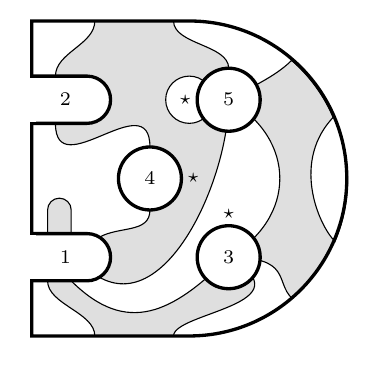
\begin{tikzpicture}[baseline = -.1cm]
	\filldraw[shaded] (.3,1.3) .. controls ++(90:.3cm) and ++(270:.3cm) .. (.8,2) -- 
		(1.8,2) .. controls ++(270:.3cm) and ++(90:.3cm) .. (2.5,1.4) --
		(2.5,1) .. controls ++(270:1cm) and ++(-30:1cm) .. (.85,-1.25) --
		(.85,-.75) .. controls ++(30:.3cm) and ++(270:.3cm) .. (1.5,-.4) -- 
		(1.5,.4) .. controls ++(90:.8cm) and ++(270:.8cm) .. (.3,.7);
	\filldraw[unshaded] (2,1) circle (.3cm);
	\filldraw[shaded] (.2,-.7) -- (.2,-.4) arc (180:0:.15cm) -- (.5,-.7);
	\filldraw[shaded]  (.2,-1.3) .. controls ++(270:.3cm) and ++(90:.3cm) .. (.8,-2) -- (1.8,-2)
		(1.8,-2) .. controls ++(90:.3cm) and ++(-30:1.2cm) .. (2.5,-1)
		.. controls ++(-135:1cm) and ++(-45:1cm) .. (.5,-1.3) -- (.2,-1.3);
	\filldraw[shaded] (2.5,1) .. controls ++(30:.3cm) and ++(-135:.3cm) .. (3.3,1.5)
		arc (49:-49:2cm)  .. controls ++(135:.3cm) and ++(0:.8cm) ..  (2.5,-1)
		.. controls ++(30:1cm) and ++(-30:1cm) .. (2.5,1);
	\filldraw[unshaded] (3.85,.8) .. controls ++(-135:.8cm) and ++(135:.3cm) .. (3.85,-.8) arc (-23:23:2cm);
%
	\halfcircle{}{(0,0)}{2}{2}{}
%
	\openhalfcircle{}{(0,1)}{.3}{.4}{\scriptsize{$2$}}
	\openhalfcircle{}{(0,-1)}{.3}{.4}{\scriptsize{$1$}}
	\ncircle{unshaded}{(2.5,1)}{.4}{180}{\scriptsize{$5$}}
	\ncircle{unshaded}{(1.5,0)}{.4}{0}{\scriptsize{$4$}}
	\ncircle{unshaded}{(2.5,-1)}{.4}{90}{\scriptsize{$3$}}
\end{tikzpicture}
\,:
(\cM_3 \otimes \cM_1) \otimes (\cP_{2,+}\otimes \cP_{1,-} \otimes \cP_{3,+}) \to \cM_{4}
$$
Here, one can glue shaded planar module tangles into the module input semidisks, and one can glue circular shaded planar tangles into the circular input disks.
In addition, the tower of algebras $(\cM_k)_{k \geq 0}$ must satisfy that multiplication in the von Neumann algebra $\cM_k$ is given by the tangle
$$
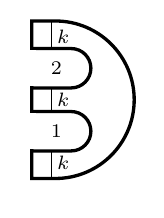
\begin{tikzpicture}[baseline = -.1cm]
	\draw (.25,-1) -- (.25,1);
%
	\halfcircle{}{(0,0)}{1}{.3}{}
%
	\openhalfcircle{}{(0,.4)}{.25}{.25}{\scriptsize{$2$}}
	\openhalfcircle{}{(0,-.4)}{.25}{.25}{\scriptsize{$1$}}
	\node at (.4,0) {\scriptsize{$k$}};
	\node at (.4,.8) {\scriptsize{$k$}};
	\node at (.4,-.8) {\scriptsize{$k$}};
\end{tikzpicture}
:
\cM_k \otimes \cM_k \to \cM_k,
$$
and the $*$-structure on $\cM_k$ is compatible with the reflection of tangles about a horizontal axis.
Notice this canonically identifies $\cM_0 = \bbC$ as a von Neumann algebra.
Under this identification, we require that the linear functionals
$$
\tr_k:=
d^{-k}\cdot\,
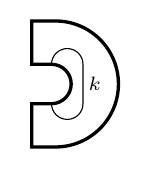
\begin{tikzpicture}[baseline = -.1cm]
	\draw (.25,.25) arc (180:0:.2cm) -- (.65,-.25) arc (0:-180:.2cm);
%
	\halfcircle{}{(0,0)}{.8}{.3}{}
%
	\openhalfcircle{}{(0,0)}{.25}{0}{}
	\node at (.8,0) {\scriptsize{$k$}};
%	\node at (.4,.8) {\scriptsize{$n$}};
%	\node at (.4,-.8) {\scriptsize{$n$}};
\end{tikzpicture}
:
\cM_k \to \cM_0 = \bbC
$$
are faithful positive normalized traces, where $d$ is the loop parameter of $\cP_\bullet$.

\nn{edit:
Prior to defining a module for a $\lambda$-lattice, in \S\ref{sec:MarkovTowers}, we define the notion of a \emph{Markov tower} $M_\bullet$, which is
a sequence of finite dimensional von Neumann algebras with faithful tracial states $(M_n, \tr_n)_{n\geq 0}$ together with a representation of Jones projections $e_n \in M_{n+1}$ for $n\geq 1$ satisfying the following properties:}
\begin{enumerate}[label={\rm(M\arabic*)}]
\item
The projections $(e_n)$ satisfy the Temperley-Lieb-Jones relations with \emph{modulus} $d>0$ (our convention for $d$ is $e_ie_{i\pm 1}e_i = d^{-2} e_i$.)
\item
For all $x\in M_n$, $e_n xe_n = E_n(x) e_n$, where $E_n: M_n \to M_{n-1}$ is the canonical trace-preserving conditional expectation.
\item
For all $n\geq 1$, $E_{n+1}(e_n) = d^{-2}$.
\item
For all $n\geq 1$, we have the Pimsner-Popa pull down property \cite{MR860811}: $M_{n+1} e_n = M_n e_n$, which is equivalent to $M_n e_n M_n$ being a 2-sided ideal in $M_{n+1}$.
\end{enumerate}
One should view a Markov tower as an analog of Popa's $\lambda$-lattices \cite{MR1334479} where we only have one tower of algebras rather than a tower/lattice of commuting squares.
Indeed, one should compare \ref{eq:MarkovJonesProjections} and \ref{eq:MarkovImplement} with (1.3.2) and \ref{eq:MarkovIndex} and \ref{eq:MarkovPullDown} with (1.3.3') from \cite{MR1334479} respectively.

Markov towers satisfy many nice properties exhibited by standard invariants of finite index ${\rm II}_1$ subfactors from \cite[Ch.~4]{MR999799}.
For example, the traces satisfy the \emph{Markov property} $\tr_{n+2}(x e_n) = d^{-2}\tr_{n+1}(x)$ for every $x\in M_{n+1}$, and the Markov tower has a \emph{principal graph} consisting of the non-reflected part of the Bratteli diagram at each step.
The tower is called \emph{finite depth} if the principal graph is finite.

The following theorem generalizes the correspondence between
unitary $2\times 2$ multitensor categories $\cC$ with $1_\cC =1_0\oplus 1_1$ and generator $X = 1_0\otimes X \otimes 1_1$ 
and
subfactor planar algebras $\cP_\bullet$.

\begin{thmalpha}
\label{thm:ModuleEquivalence}
Let $\cP_\bullet$ be a subfactor planar algebra corresponding to $(\cC, X)$ as above.
There is an equivalence between:
\begin{enumerate}[label={\rm(\arabic*)}]
\item
pivotal right $\cC$-module $\Cstar$ categories $(\cM,\Tr^\cM)$ with choice of simple basepoint $m = m\vartriangleleft 1_0$, and
\item
connected right planar modules $\cM_\bullet$ for $\cP_\bullet$
%\item
%cyclic right lattice modules $M_\bullet$ for $\cA_{\bullet, \bullet}$.
\end{enumerate}
\end{thmalpha}

\nn{edit:
In fact, any Markov tower of modulus $d$
 is automatically equipped with the structure of a cyclic right lattice module for 
the Temerley-Lieb-Jones $d^{-2}$-lattice $TLJ(d)_\bullet$.
Moreover, any pointed bipartite graph $(\Gamma,v)$ with a \emph{quantum dimension function} on vertices $\dim: V(\Gamma) \to \bbR_{>0}$ satisfying
$$
d\cdot \dim(v) = \sum_{w\sim v} \dim(w)
$$
gives us a Markov tower of modulus $d$, where we write $w\sim v$ to mean $w$ is connected to $v$, and the sum is taken with multiplicity.
We thus get the following corollary, which should be compared with the non-pivotal case in \cite{MR3420332}.
}

\begin{coralpha}
\label{cor:TLJPivotalModuleClassification}
There is a bijective correspondence between
pivotal $\cT\cL\cJ(d)$-module $\Cstar$ categories with basepoint and 
pointed connected bipartite graphs $(\Gamma, v)$ with a quantum dimension function.
\end{coralpha}

One passes from (2) or (3) to (1) in Theorem \ref{thm:ModuleEquivalence} by taking the category of projections, similar to the correspondence between $\cP_\bullet$ or $A_{\bullet,\bullet}$ and $(\cC, X)$.
One passes from (1) to (2) using the diagrammatic calculus, similar to how one gets a subfactor planar algebra from $(\cC, X)$ \cite{MR2811311,1808.00323}.
We rapidly sketch how to pass from (3) to (1), as it will be useful for our proof of the module embdedding theorem.


%Suppose $\cQ_\bullet$ is a finite depth subfactor planar algebra, and let $\cC$ be its associated $2\times 2$ unitary multifusion category of projections with generator $c$ corresponding to the unshaded-shaded strand in $\cQ_{1,+}$.
%Here, $1_\cC$ decomposes as an orthogonal direct sum $1_\cC = 1_0\oplus 1_1$, which decomposes $\cC= \bigoplus_{i,j=0}^1 \cC_{ij}$ where $\cC_{ij}:= 1_i \otimes \cC \otimes 1_j$.
%By a %Here, we use the graphical notation of \nn{}, where coupons in $\cM$ have no boundary on the left to indicate the absence of a left $\cC$-action.

From the pivotal semisimple right $\cC$-module $\Cstar$ category $(\cM, \Tr^\cM)$ together with a choice of simple object $m\in \cM$ with $m= m\vartriangleleft 1_0$, we build a Markov tower $M_\bullet$ by setting
$$
M_n := \End_\cM(m \vartriangleleft  \underbrace{X\otimes \overline{X} \otimes \cdots \otimes X^?}_{n \text{ tensorands}})
$$
where for our generator $X\in \cC$, $X^? = X$ if $n$ is even and $X^? = \overline{X}$ if $n$ is odd.
The trace $\Tr^\cM$ endows each von Neumann algebra $M_n$ with a faithful tracial state $\tr_n := \Tr^\cM(\id_n)^{-1} \Tr^\cM$ together with canonical Jones projections $e_n \in M_{n+1}$ for all $n\geq 1$.
Based on the parity of $n$, the $e_n$ are defined for $k\geq 0$ by
\begin{align*}
e_{2k+1}
&=
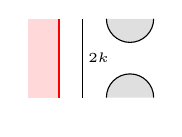
\begin{tikzpicture}[baseline]
	\fill[ctwoshading] (-.3,-.5) rectangle (-.7,0.5);
	\draw[thick,red] (-0.3,-.5) -- (-0.3,0.5);
	\draw (0,-.5) -- (0,.5);
	\filldraw[shaded] (.3,.5) arc (-180:0:.3cm);
	\filldraw[shaded] (.3,-.5) arc (180:0:.3cm);
	\node at (.2,0){\tiny{$2k$}};
\end{tikzpicture} 
\hspace{.3cm}
:=
d^{-1}
\big(
\id_m \vartriangleleft \id_{(X\otimes \overline{X})^{\otimes k}} \otimes (\coev_X \circ \coev_X^\dag)
\big)
\in M_{2k+2}
\\
e_{2k+2}
&=
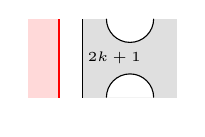
\begin{tikzpicture}[baseline]
	\fill[ctwoshading] (-.3,-.5) rectangle (-.7,0.5);
	\fill[shaded] (0,-.5) rectangle (1.2,.5);
	\draw[thick,red] (-0.3,-.5) -- (-0.3,0.5);
	\draw (0,-.5) -- (0,.5);
	\filldraw[unshaded] (.3,.5) arc (-180:0:.3cm);
	\filldraw[unshaded] (.3,-.5) arc (180:0:.3cm);
	\node at (.4,0){\tiny{$2k+1$}};
\end{tikzpicture} 
:=
d^{-1}
\big(
\id_m \vartriangleleft \id_X \otimes \id_{(\overline{X}\otimes X)^{\otimes k}} \otimes (\ev_X^\dag \circ \ev_X)
\big)
\in M_{2k+3}.
\end{align*}
Here, $(\overline{X}, \ev_X, \coev_X)$ is the balanced dual of $X$, $m$ is graphically represented by a red strand, and the left hand side of $m$ is shaded to denote the absence of a left $\cC$-action.
It is straightforward to verify $M_\bullet := (M_n,\tr_n, e_{n+1})_{n\in \bbN}$ is a Markov tower.
%We call the tower of algebras with Jones projections $(M_n,\tr_n, e_{n+1})_{n\in \bbN}$ a \emph{Markov tower}, as it satisfies the following properties:
%\begin{enumerate}[label={\rm(\arabic*)}]
%\item
%The projections $(e_n)$ satisfy the Temperley-Lieb-Jones relations with parameter $d>0$ (our convention for $d$ is $e_ie_{i\pm 1}e_i = d^{-2} e_i$.)
%\item
%For all $x\in M_n$, $e_n xe_n = E_n(x) e_n$, where $E_n: M_n \to M_{n-1}$ is the canonical trace-preserving conditional expectation.
%\item
%For all $n\geq 1$, $E_{n+1}(e_n) = d^{-2}$.
%\item
%For all $n\geq 1$, we have the Pimsner-Popa pull down property: $M_{n+1} e_n = M_n e_n$, which is equivalent to $M_n e_n M_n$ being a 2-sided ideal in $M_{n+1}$.
%\end{enumerate}
%One should view a Markov tower as an analog of Popa's \emph{$\lambda$-sequence/lattice} \cite{MR1334479} where we only have one tower of algebras rather than a tower/lattice of commuting squares.
%Markov towers satisfy many nice properties exhibited by standard invariants of finite index ${\rm II}_1$ subfactors from \cite[Ch.~4]{MR999799}.
%For example, the traces satisfy the \emph{Markov property} $\tr_{n+2}(x e_n) = d^{-2}\tr_{n+1}(x)$ for every $x\in M_{n+1}$, and the Markov tower has a \emph{principal graph} consisting of the non-reflected part of the Bratteli diagram at each step.
%We refer the reader to \S\ref{sec:MarkovTowers} for more details on Markov towers of finite dimensional von Neumann algebras.

We now specialize to the hypotheses of the module embedding theorem, i.e., $\cP_\bullet$ is a finite depth subfactor planar algebra and $\cM$ is finitely semisimple.
In this case, the Markov tower $M_\bullet$ constructed above has finite depth, and its principal graph $\Gamma$ is equal to the \emph{fusion graph} of $(\cM,m)$ with respect to $X\in \cC$.
This means there is an $r>0$ such that the inclusion $M_{2r} \subset (M_{2r+1}, \tr_{2r+1})$ is \emph{strongly Markov}, meaning that there is a finite \emph{Pimsner-Popa basis} $\{b\}$ for $M_{2r+1}$ over $M_{2r}$ satisfying $\sum_b be_{2r} b^* = 1_{M_{2r+2}}$, and the \emph{Watatani index} $\sum_b bb^*$ \cite{MR996807} is a scalar.
We refer the reader to \cite[1.1.4(c)]{MR1278111} for other equivalent properties for the Watatani index in the presence of a Pimsner-Popa basis. 

By \cite[\S2.3]{MR2812459}, the inclusion $A_0:=M_{2r} \subset (M_{2r+1}, \tr_{2r+1}) =: (A_1, \tr_1)$ has a canonical associated planar $\dag$-algebra $\cQ_\bullet$, which is built from the tower of higher relative commutants.
Moreover, by \cite[Thm.~3.8]{MR2812459}, the planar algebra $\cQ_\bullet$ is \emph{non-canonically} isomorphic to the bipartite graph planar algebra $\cG_\bullet$ of the Bratteli diagram of the inclusion $A_0 \subset A_1$, which is also the fusion graph $\Gamma$. 
(This isomorphism depends on the loop algebra representation for $A_0 \subset A_1$ from \cite[\S3.1]{MR2812459}, which amounts to choosing compatible bases for the algebras.)
%Notice that we may canonically identify $\Gamma$ with the principal graph of the Markov tower $M_\bullet$ and the fusion graph for $(\cM,m)$ with respect to $c\in \cC$.

%We are now in the position to state the embedding theorem for module categories for a finite depth subfactor planar algebra $\cP_\bullet$.

\begin{thmalpha}
The unital $*$-algebra maps $\Phi_{n,\pm}:= \id_m \vartriangleleft \id_{(X\otimes \overline{X})^{\otimes r}}\vartriangleleft - : \cP_{n,\pm} \to \cQ_{n,\pm}$
$$
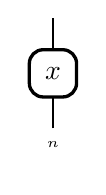
\begin{tikzpicture}[baseline]
	\draw (0,-.7) -- (0,.7);
	\roundNbox{unshaded}{(0,0)}{.3}{0}{0}{$x$}
	\node at (0,-.9) {\tiny{$n$}};
\end{tikzpicture}
\quad
\begin{tikzpicture}[baseline]
	\clip (0.5,0.9) -- (-0.5,0.9) -- (-0.5,-0.9) -- (0.5,-0.9);
	\draw [|->,thick] (-0.3,0)--(0.3,0);
	\node at (0,0.25) {\scriptsize{$\Phi$}};
\end{tikzpicture}
\quad
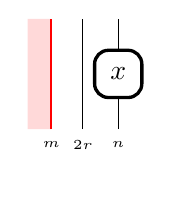
\begin{tikzpicture}[baseline]
	\fill[ctwoshading] (-.4,-.7) -- (-0.4,.7) -- (-.7,0.7) -- (-.7,-0.7) -- (-.4,-0.7);
	\draw[thick,red] (-0.4,-.7) -- (-0.4,0.7);
	\draw (0.45,-.7) -- (0.45,.7);
	\draw (0,-.7) -- (0,.7);
	\roundNbox{unshaded}{(0.45,0)}{.3}{0}{0}{$x$}
	\node at (0.45,-.9) {\tiny{$n$}};
	\node at (0,-0.9){\tiny{$2r$}};
	\node at (-0.4,-.9) {\tiny{$m$}};
\end{tikzpicture} 
$$
give a planar $\dag$-algebra embedding $\cP_\bullet \hookrightarrow \cQ_\bullet$.
\end{thmalpha}

Choosing $\cM = \cC_{00}\oplus \cC_{10}$ and $m = 1_{\cC_{00}}$ corresponding to the unshaded empty diagram exactly recovers the embedding into the graph planar algebra of the principal graph of $\cP_\bullet$ from \cite{MR2812459}.
Similarly, we get an embedding into the graph planar algebra of the dual principal graph from choosing $\cM= \cC_{10} \oplus \cC_{11}$ and $m \in \cC_{10}$ is an arbitrary choice of simple object.

\nn{invariance of embedding. 
explain conceptual origin of above embedding map from shift iso.}

%%%%%%%%%%%%%%%%%%%%%%%%%%%%%%%%%%%%%%%%%%%%%%%%%%%%%%%
\paragraph{Acknowledgements.}

\nn{todo}



%%%%%%%%%%%%%%%%%%%%%%%%%%%%%%%%%%%%%%%%%%%%%%%%%%%%%%%
%%%%%%%%%%%%%%%%%%%%%%%%%%%%%%%%%%%%%%%%%%%%%%%%%%%%%%%
%%%%%%%%%%%%%%%%%%%%%%%%%%%%%%%%%%%%%%%%%%%%%%%%%%%%%%%
\section{Modules for standard invariants of subfactors} 
\label{sec:Modules}

\nn{the standard invariant of a finite index subfactor}

%%%%%%%%%%%%%%%%%%%%%%%%%%%%%%%%%%%%%%%%%%%%%%%%%%%%%%%
\subsection{Unitary multitensor categories and subfactor planar algebras}  
\label{sec:CategoriesPlanarAlgberasLattices}

In this section, we rapidly recall the definitions of a subfactor planar algebra \cite{math.QA/9909027} and its unitary $2\times 2$ multitensor category of projections \cite{MR2811311,1808.00323}.

\begin{defn}
The \emph{shaded planar operad} consists of shaded planar tangles with the operation of composition.
Shaded planar tangles have $r\geq 0$ input disks each with $2k_i$ boundary points, and an output disk with $2k_0$ boundary points.
Internal to the output disk are non-intersecting strings, which either attach 2 distinct boundary points, or are closed loops.
There is also a checkerboard shading, and a distinguished interval marked $\star$ for each input disk and the output disk.
If the $\star$ for the $i$-th disk is on an interval which meets an unshaded region, that disk has \emph{type} $(k_i, +)$, and if it meets a shaded region, the disk has type $(k_i,-)$.
There is a natural definition of the composite tangle $T \circ_i S$ when the output disk of a tangle $T$ has the same type as the $i$-th input disk of a tangle $T$.
We give a representative example below, and we refer the reader to \cite{MR2679382,MR2972458} for a more precise definition.
$$
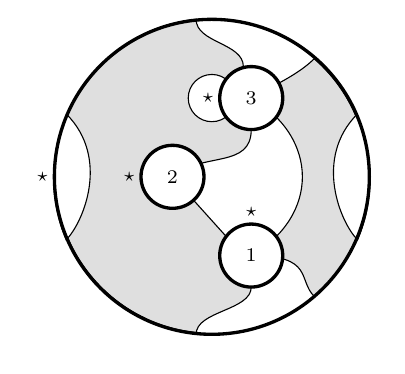
\begin{tikzpicture}[baseline = -.1cm]
	\filldraw[shaded]  
		(1.8,-2) .. controls ++(90:.3cm) and ++(-90:.3cm) .. (2.5,-1.4) -- (2.4,-1) -- 
		(1.5,0) .. controls ++(40:.5cm) and ++(270:.5cm) .. (2.5,.6) -- 
		(2.4,1.4) .. controls ++(90:.3cm) and ++(270:.3cm) .. (1.8,2) arc (96:264:2cm) ;
	\filldraw[unshaded] (2,1) circle (.3cm);
	\filldraw[shaded] (2.5,1) .. controls ++(30:.3cm) and ++(-135:.3cm) .. (3.3,1.5)
		arc (49:-49:2cm)  .. controls ++(135:.3cm) and ++(0:.8cm) ..  (2.5,-1)
		.. controls ++(30:1cm) and ++(-30:1cm) .. (2.5,1);
	\filldraw[unshaded] (3.85,.8) .. controls ++(-135:.8cm) and ++(135:.3cm) .. (3.85,-.8) arc (-23:23:2cm);
	\filldraw[unshaded] (.15,.8) .. controls ++(-45:.8cm) and ++(45:.3cm) .. (.15,-.8) arc (203:157:2cm);
%
	\ncircle{}{(2,0)}{2}{180}{}
%
	\ncircle{unshaded}{(2.5,1)}{.4}{180}{\scriptsize{$3$}}
	\ncircle{unshaded}{(1.5,0)}{.4}{180}{\scriptsize{$2$}}
	\ncircle{unshaded}{(2.5,-1)}{.4}{90}{\scriptsize{$1$}}
\end{tikzpicture}
\circ_{3}
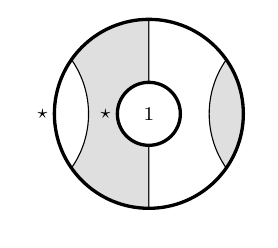
\begin{tikzpicture}[baseline = -.1cm]
	\filldraw[shaded] (0,-1.2) -- (0,1.2) arc (90:270:1.2cm);
	\filldraw[unshaded] (145:1.2cm) arc (145:215:1.2cm) arc (-35:35:1.2cm);
	\filldraw[unshaded] (0,-1.2) -- (0,1.2) arc (90:-90:1.2cm);
	\filldraw[shaded] (35:1.2cm) arc (35:-35:1.2cm) arc (215:145:1.2cm);
%
	\ncircle{}{(0,0)}{1.2}{180}{}
%
	\ncircle{unshaded}{(0,0)}{.4}{180}{\scriptsize{$1$}}
\end{tikzpicture}
=
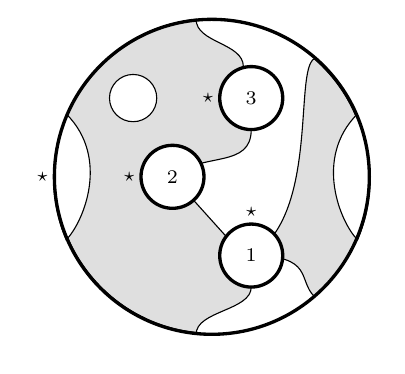
\begin{tikzpicture}[baseline = -.1cm]
	\filldraw[shaded]  
		(1.8,-2) .. controls ++(90:.3cm) and ++(-90:.3cm) .. (2.5,-1.4) -- (2.4,-1) -- 
		(1.5,0) .. controls ++(40:.5cm) and ++(270:.5cm) .. (2.5,.6) -- 
		(2.4,1.4) .. controls ++(90:.3cm) and ++(270:.3cm) .. (1.8,2) arc (96:264:2cm) ;
	\filldraw[unshaded] (1,1) circle (.3cm);
	\filldraw[shaded] (3.3,1.5)	arc (49:-49:2cm)  .. controls ++(135:.3cm) and ++(0:.8cm) ..  (2.5,-1)
		.. controls ++(30:1cm) and ++(210:.3cm) .. (3.3,1.5);
	\filldraw[unshaded] (3.85,.8) .. controls ++(-135:.8cm) and ++(135:.3cm) .. (3.85,-.8) arc (-23:23:2cm);
	\filldraw[unshaded] (.15,.8) .. controls ++(-45:.8cm) and ++(45:.3cm) .. (.15,-.8) arc (203:157:2cm);
%
	\ncircle{}{(2,0)}{2}{180}{}
%
	\ncircle{unshaded}{(2.5,1)}{.4}{180}{\scriptsize{$3$}}
	\ncircle{unshaded}{(1.5,0)}{.4}{180}{\scriptsize{$2$}}
	\ncircle{unshaded}{(2.5,-1)}{.4}{90}{\scriptsize{$1$}}
\end{tikzpicture}
$$

A \emph{shaded planar algebra} $\cP_\bullet$ consists of a family $\cP_{n,\pm}$ of $\bbC$-vector spaces together with an action of the shaded planar operad.
That is, each shaded planar tangle $T$ with input disks of type $(k_i, \pm_i)$ for $1\leq i\leq r$ and output disk of type $(k_0,\pm_0)$ defines a multilinear map $Z(T) : \prod_{i=1}^r \cP_{k_i, \pm_i} \to \cP_{k_0, \pm_0}$, and tangle composition corresponds to composition of multilinear maps.
\end{defn}

\begin{nota}
We will try to shade our diagrams as much as possible for a shaded planar algebra.
However, sometimes shading our diagrams requires us to split into many cases.
In order to avoid this, we sometimes suppress the shading when it can be inferred from the indices.
We also tend to suppress the external boundary disk of a shaded planar tangle; when we do so, the $\star$ is always on the left.
For explicit examples, compare \ref{PA:Positive} and \ref{PA:Spherical} in the following definition.
\end{nota}

\begin{defn}
A shaded planar algebra is called a \emph{subfactor planar algebra} if moreover
\begin{enumerate}[label={\rm(PA\arabic*)}]
\item
(finite dimensional) $\dim(\cP_{n,\pm}) <\infty$ for all $n\geq 0$.
\item
(evaluable/connected) $\dim(\cP_{0,\pm}) = 1$.
\item
\label{PA:Positive}
(positive)
$\langle x, y\rangle_{n,\pm} := 
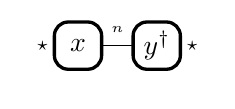
\begin{tikzpicture}[baseline=-.1cm]
	\draw (0,0) -- (.8,0);
	\roundNbox{unshaded}{(0,0)}{.3}{0}{0}{$x$}
	\roundNbox{unshaded}{(1,0)}{.3}{0}{0}{$y^\dag$}
	\node at (.5,.2){\tiny{$n$}};
	\node at (-.45,0){\scriptsize{$\star$}};
	\node at (1.45,0){\scriptsize{$\star$}};
\end{tikzpicture}
$
defines a positive-definite inner product on each $\cP_{n,\pm}$.
\item
\label{PA:Spherical}
(spherical)
for all $x\in \cP_{1,+}$, 
$
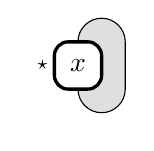
\begin{tikzpicture}[baseline=-.1cm]
	\filldraw[shaded] (0,.3) arc (180:0:.3cm) -- (.6,-.3) arc (0:-180:.3cm);
	\roundNbox{unshaded}{(0,0)}{.3}{0}{0}{$x$}
	\node at (-.45,0){\scriptsize{$\star$}};
\end{tikzpicture}
=
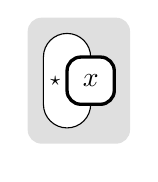
\begin{tikzpicture}[baseline=-.1cm]
	\fill[shaded, rounded corners = 5pt] (-.8,-.8) rectangle (.5,.8);
	\filldraw[unshaded] (0,.3) arc (0:180:.3cm) -- (-.6,-.3) arc (-180:0:.3cm);
	\roundNbox{unshaded}{(0,0)}{.3}{0}{0}{$x$}
	\node at (-.45,0){\scriptsize{$\star$}};
\end{tikzpicture}
$.
\end{enumerate}
In a subfactor planar algebra, closed contractible loops can be traded for a multiplicative scalar $d>0$.
By Jones' index rigidity theorem \cite{MR0696688}, $d\in \set{2\cos(\pi/k)}{k\geq 3}\cup [2,\infty)$.

Given a subfactor planar algebra $\cP_\bullet$, we get two Markov towers $\cP_\pm= (\cP_{n,\pm})_{n\geq 0}$ 
with Jones projections for $k\geq 0$ given by
\begin{equation}
\label{eq:JonesProjectionsForPlanarAlgebra}
e_{2k+1,+}
:=
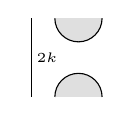
\begin{tikzpicture}[baseline]
	\draw (0,-.5) -- (0,.5);
	\filldraw[shaded] (.3,.5) arc (-180:0:.3cm);
	\filldraw[shaded] (.3,-.5) arc (180:0:.3cm);
	\node at (.2,0){\tiny{$2k$}};
\end{tikzpicture} 
\qquad
e_{2k+2,+}
:=
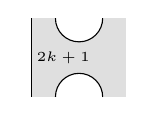
\begin{tikzpicture}[baseline]
	\fill[shaded] (0,-.5) rectangle (1.2,.5);
	\draw (0,-.5) -- (0,.5);
	\filldraw[unshaded] (.3,.5) arc (-180:0:.3cm);
	\filldraw[unshaded] (.3,-.5) arc (180:0:.3cm);
	\node at (.4,0){\tiny{$2k+1$}};
\end{tikzpicture} 
\qquad
e_{2k+1,-}:=
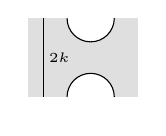
\begin{tikzpicture}[baseline]
	\fill[shaded] (-.2,-.5) rectangle (1.2,.5);
	\draw (0,-.5) -- (0,.5);
	\filldraw[unshaded] (.3,.5) arc (-180:0:.3cm);
	\filldraw[unshaded] (.3,-.5) arc (180:0:.3cm);
	\node at (.2,0){\tiny{$2k$}};
\end{tikzpicture} 
\qquad
e_{2k+2,-}:=
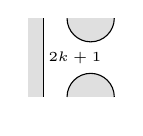
\begin{tikzpicture}[baseline]
	\fill[shaded] (-.2,-.5) rectangle (0,.5);
	\draw (0,-.5) -- (0,.5);
	\filldraw[shaded] (.3,.5) arc (-180:0:.3cm);
	\filldraw[shaded] (.3,-.5) arc (180:0:.3cm);
	\node at (.4,0){\tiny{$2k+1$}};
\end{tikzpicture}
\end{equation}
and traces for $n\geq 0$ given by
\begin{equation}
\label{eq:TracesForPlanarAlgebra}
\tr_{n,\pm}:= d^{-n}\,
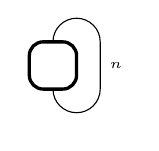
\begin{tikzpicture}[baseline=-.1cm]
	\draw (0,.3) arc (180:0:.3cm) -- (.6,-.3) arc (0:-180:.3cm);
	\roundNbox{unshaded}{(0,0)}{.3}{0}{0}{}
	\node at (.8,0){\tiny{$n$}};
\end{tikzpicture} \,.
\end{equation}
The principal graph of $\cP_+$ is finite if and only if the principal graph of $\cP_-$ is finite; in this case, $\cP_\bullet$ is said to have \emph{finite depth}.
\end{defn}


\begin{defn}\label{def:multitensor}
A \emph{unitary $2\times 2$ multitensor category} $\cC$ is an indecomposable rigid $\Cstar$ tensor category which is Karoubi complete such that $1_\cC$ has an orthogonal decomposition into simple objects as $1_\cC = 1_0 \oplus 1_1$.
We write $\cC_{ij} := 1_i \otimes \cC \otimes 1_j$ for $i,j \in \{0,1\}$.
By \cite{MR1444286}, such a $\cC$ is automatically semisimple.
When $\cC$ is finitely semisimple, it is called a unitary $2\times 2$ \emph{multifusion} category \cite{egno}.

We say $X\in \cC_{01}$ \emph{generates} $\cC$ if every object of $\cC$ is isomorphic to a direct summand of an alternating tensor power of $X$ and $\overline{X}$
$$
X^{ \text{alt}\otimes n}
:=
\underbrace{X\otimes \overline{X} \otimes \cdots \otimes X^?}_{n\text{ tensorands}}
\qquad
\qquad
\overline{X}^{ \text{alt}\otimes n}
:=
\underbrace{\overline{X} \otimes X\otimes \cdots \otimes \overline{X}^?}_{n\text{ tensorands}}
$$
where $X^? = X$ if $n$ is odd and $\overline{X}$ when $n$ is even, and $\overline{X}^? = \overline{X}$ when $n$ is odd and $X$ when $n$ is even.
Here, $(\overline{X}, \ev_X, \coev_X)$ is the canonical \emph{balanced} dual of $X$ \cite{MR3342166,1805.09234,1808.00323} which satisfies the zig-zag axioms and the balancing equation
$$
\psi(\ev_X \circ (\id_{\overline{X}} \otimes f) \circ \ev_X^\dag)
=
\psi(\coev_X^\dag \circ (f\otimes \id_{\overline{X}}) \circ \coev_X)
\qquad
\forall f\in \cC(X\to X)
$$
where $\psi : \cC(1_\cC\to 1_\cC) \to \bbC$ is the linear functional such that $\psi(\id_{1_0}) = \psi(\id_{1_1}) = 1$.
\end{defn}

The following theorem is well-known to experts.

\begin{thm}
There is an equivalence of categories\,\footnote{We suppress the subtlety about the right hand side of this equivalence being a contractible 2-category. 
We refer the reader to \cite{1607.06041,1808.00323} for more details.}
\[
\left\{\, 
\parbox{4.8cm}{\rm Subfactor planar algebras $\cP_\bullet$}\,\left\}
\,\,\,\,\cong\,\,
\left\{\,\parbox{7.5cm}{\rm Pairs $(\cC, X)$ with $\cC$ a unitary $2\times 2$ multitensor category together with a generator $X\in \cC_{01}$}\,\right\}.
\right.\right.
\]
\end{thm}

Starting with a subfactor planar algebra $\cP_\bullet$, one may form its unitary $2\times 2$ multitensor category of projections $\cC$ \cite{MR2559686,MR3405915,1808.00323}, which comes with a canonical generator corresponding to the unshaded-shaded strand in $\cP_{1,+}$, and the canonical spherical unitary dual functor \cite{MR3342166,1805.09234,1808.00323}.
This unitary $2\times 2$ multitensor category can also be thought of as a unitary 2-category called the \emph{paragroup}; we refer the reader to \cite{MR3157990} for more details.

Starting with a pair $(\cC, X)$, we get a subfactor planar algebra by defining
$$
\cP_{n,+} := \End_\cC(X^{ \text{alt} \otimes n})
\qquad\qquad
\cP_{n,-} := \End_\cC(\overline{X}^{ \text{alt} \otimes n}),
$$
and we define the action of the shaded planar operad via the diagrammatic calculus for pivotal tensor categories.
We refer the reader to \cite{MR2811311,1808.00323} for more details.

%%%%%%%%%%%%%%%%%%%%%%%%%%%%%%%%%%%%%%%%%%%%%%%%%%%%%%%
\subsection{Modules for unitary multitensor categories and subfactor planar algebras}
\label{ssec:moduledefs}
\label{sec:3TypesOfModules}

We now define the various notions of module for 
\begin{itemize}
\item
a unitary $2\times 2$ multitensor category $\cC$ with its canonical unitary spherical structure and a generator $X\in \cC_{01}$,
and
\item
a subfactor planar algebra $\cQ_\bullet$.
\end{itemize}

\begin{defn}
Let $\cC$ be a unitary $2\times 2$ multitensor category.
A \emph{pivotal right $\cC$-module $\Cstar$ category} is a pair $(\cM,\Tr^\cM)$ where
$\cM$ is a semisimple right $\cC$-module $\Cstar$ category, and $\Tr^\cM$ is a family of positive traces $\Tr^\cM_n:\cM(n \to n)\to \bbC$ on each endomorphism space for $n\in \cM$ satisfying the following axioms:
\begin{itemize}
\item
(tracial)
$\Tr^\cM_m(g \circ f) = \Tr^\cM_n(f\circ g)$ for all $f\in \cM(m\to n)$ and $g\in \cM(n \to m)$.
\item
(positive)
$\Tr^\cM_m(f^\dag \circ f) \geq 0$ for all $f\in \cM(m \to n)$, and $\Tr^\cM_m(f^\dag \circ f) =0$ if and only if $f = 0$.
%\item
%(normalized)
%$\Tr^\cM_m( \id_m) = 1_\bbC$.
\item
(compatible with $\cC$)
For all $m\in \cM$ and $c\in \cC$,
$
\Tr^\cM_{m\vartriangleleft c}(f)
=
\Tr^\cM_{m}(
(\id_m \otimes \coev_c^\dag) \circ (f\otimes \id_{\overline{c}}) \circ (\id_m \vartriangleleft \coev_c)
)
$
\end{itemize}
Notice that $\cM = \cM_0 \oplus \cM_1$ where $\cM_0 = \cM \vartriangleleft 1_0$ and $\cM_1 = \cM\vartriangleleft 1_1$.

A pivotal right module category is called \emph{pointed} if it is indecomposable, we have a chosen simple object $m\in \cM$, and $\Tr^\cM$ is normalized so that $\Tr^\cM_m(\id_m) = 1_\bbC$.
Generally, we choose $m\in \cM_0$, but this choice is not essential.

When $\cC$ is generated by a single $X\in \cC_{01}$ and $(\cM,\Tr^\cM,m)$ is a pointed pivotal right module category with $m\in \cM_0$, we define the \emph{cyclic pivotal right module category} $\cM_{m,X}$ to be the (non Karoubi complete!) full subcategory of $\cM$ whose objects are of the form 
$
m \vartriangleleft X^{ \text{alt}\otimes k}
$ 
for $k\geq 0$, which is a pointed pivotal right module category over $\cC_X$, the (non Karoubi complete!) full subcategory of $\cC$ whose objects are of the form $X^{ \text{alt}\otimes k}$ and $\overline{X}^{ \text{alt}\otimes k}$ for $k\geq 0$.
\end{defn}


We next give an appropriate definition of planar modules over a planar algebra as algebras over another operad.
\footnote{Our definition of a planar module over a planar algebra differs significantly from the annular planar modules introduced in \cite{MR1929335}. Our planar modules will correspond to the above notion of module over a multitensor category, whereas annular planar modules correspond to algebra objects in the Drinfel'd center of such a category. \nn{Add a citation for details.}}

\begin{defn}
\label{def:PlanarModule}
	The \textit{shaded planar module operad} is a variant of the shaded planar operad, akin to a shaded, stranded version of the Swiss-cheese operad introduced in \cite{MR1718089}. In this operad, the starred region of the boundary of the output disk of a tangle is replaced by a vertical line on the left side of a tangle, and the adjacent region inside the tangle must be unshaded. In addition to the usual input disks, tangles may also have input semidisks, whose boundaries intersect the left wall. The operadic composition comes from plugging tangles into semidisks. A representative tangle appears below. 
\end{defn}
$$
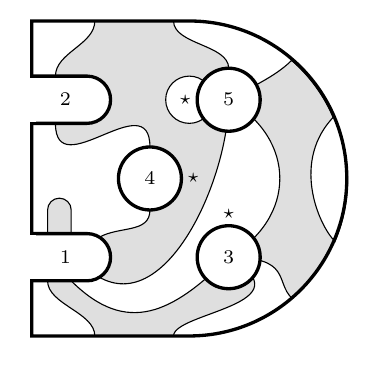
\begin{tikzpicture}[baseline = -.1cm]
	\filldraw[shaded] (.3,1.3) .. controls ++(90:.3cm) and ++(270:.3cm) .. (.8,2) -- 
		(1.8,2) .. controls ++(270:.3cm) and ++(90:.3cm) .. (2.5,1.4) --
		(2.5,1) .. controls ++(270:1cm) and ++(-30:1cm) .. (.85,-1.25) --
		(.85,-.75) .. controls ++(30:.3cm) and ++(270:.3cm) .. (1.5,-.4) -- 
		(1.5,.4) .. controls ++(90:.8cm) and ++(270:.8cm) .. (.3,.7);
	\filldraw[unshaded] (2,1) circle (.3cm);
	\filldraw[shaded] (.2,-.7) -- (.2,-.4) arc (180:0:.15cm) -- (.5,-.7);
	\filldraw[shaded]  (.2,-1.3) .. controls ++(270:.3cm) and ++(90:.3cm) .. (.8,-2) -- (1.8,-2)
		(1.8,-2) .. controls ++(90:.3cm) and ++(-30:1.2cm) .. (2.5,-1)
		.. controls ++(-135:1cm) and ++(-45:1cm) .. (.5,-1.3) -- (.2,-1.3);
	\filldraw[shaded] (2.5,1) .. controls ++(30:.3cm) and ++(-135:.3cm) .. (3.3,1.5)
		arc (49:-49:2cm)  .. controls ++(135:.3cm) and ++(0:.8cm) ..  (2.5,-1)
		.. controls ++(30:1cm) and ++(-30:1cm) .. (2.5,1);
	\filldraw[unshaded] (3.85,.8) .. controls ++(-135:.8cm) and ++(135:.3cm) .. (3.85,-.8) arc (-23:23:2cm);
%
	\halfcircle{}{(0,0)}{2}{2}{}
%
	\openhalfcircle{}{(0,1)}{.3}{.4}{\scriptsize{$2$}}
	\openhalfcircle{}{(0,-1)}{.3}{.4}{\scriptsize{$1$}}
	\ncircle{unshaded}{(2.5,1)}{.4}{180}{\scriptsize{$5$}}
	\ncircle{unshaded}{(1.5,0)}{.4}{0}{\scriptsize{$4$}}
	\ncircle{unshaded}{(2.5,-1)}{.4}{90}{\scriptsize{$3$}}
\end{tikzpicture}
\,:
(\cM_3 \otimes \cM_1) \otimes (\cP_{2,+}\otimes \cP_{1,-} \otimes \cP_{3,+}) \to \cM_{4}
$$
Tangles of the shaded planar module operad can also be composed with shaded planar tangles, by plugging a shaded planar tangle into an input disk. 
One should think of the box spaces for semidisks as being endomrphisms of objects in a module category, while the involvement of full disks allows a planar algebra to act on the module. 
The input disks and semidiscs are also numbered, with the numbering determining the order of the tensor factors in the domain of the action map as depicted above. Like the shaded planar operad, the shaded planar module operad is a symmetric operad, and vectorspaces form a symmetric monoidal category, so we often supress the numbering. 

\begin{defn}
A \emph{right planar module} $\cM_\bullet$ for the subfactor planar algebra $\cP_\bullet$ consists of a sequence of $\bbC$-vector spaces $(M_k)_{k\geq 0}$
together with an action of the shaded planar module operad on the box spaces $\cM_\bullet$ and $\cP_\bullet$ compatible with the composition of tangles and the shaded planar algebra structure on $\cP_\bullet$. In other words, the box spaces $\cM_\bullet$ and $\cP_\bullet$ together must have the structure of an algebra over the shaded planar module operad, which must extend the original shaded planar operad algebra structure on $\cP_\bullet$. 
\end{defn}

\begin{ex}
	Given a subfactor planar algebra $\cP_\bullet$, the even part of $\cP_\pm :=( \cP_{k,\pm})_{k\geq 0}$ is a cyclic right planar modules for $\cP_\bullet$, while the odd part is a right planar module for the dual planar algebra $\cP_{\mp}$. 
\end{ex}

\begin{ex}
Suppose $\cG_\bullet =\cG\cP\cA(\Gamma)_\bullet$ is the graph planar algebra of the bipartite graph $\Gamma$, and denote its Jones projections by $g_{n,\pm}$.
Then for any $\pm$ vertex $v$ of $\Gamma$, we get a cyclic right planar module $\cM_\bullet = \cM(\Gamma,v)_\bullet$ by defining $\cM(\Gamma, v)_{k}:= p_v \cG_{k,\pm}$ and action of the planar module operad by
$$
Z_{\cM_\bullet}(\cT)
\left(
\underbrace{m_1\otimes \cdots \otimes m_r}_{\in \cM_\bullet} 
\otimes 
\underbrace{x_1\otimes \cdots\otimes x_s}_{\in \cP_\bullet}
\right)
:=
Z_{\cG_\bullet}(\widetilde{\cT})(p_v\otimes m_1\otimes \cdots \otimes m_r \otimes \Phi(x_1)\otimes \cdots\otimes \Phi(x_s))
$$
where $\widetilde{\cT}$ is obtained from $\cT$ by 
first turning each half-open input semidisk into a closed input disk in the interior of the output disk with its $\star$ on the left, 
rounding out the $90^\circ$ angles on the left boundary into a smooth curve,
putting the external $\star$ on the left hand side,
and inserting one $(0,+)$-type input disk in the left-most region of the new tangle which is numbered first.
We illustrate this procedure on the tangle above:
$$
\cT=
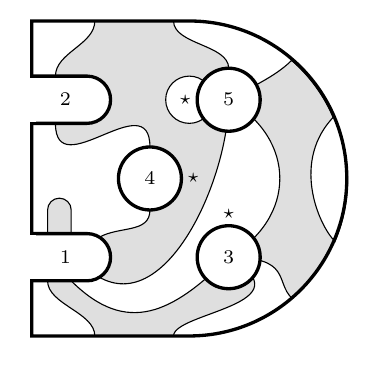
\begin{tikzpicture}[baseline = -.1cm]
	\filldraw[shaded] (.3,1.3) .. controls ++(90:.3cm) and ++(270:.3cm) .. (.8,2) -- 
		(1.8,2) .. controls ++(270:.3cm) and ++(90:.3cm) .. (2.5,1.4) --
		(2.5,1) .. controls ++(270:1cm) and ++(-30:1cm) .. (.85,-1.25) --
		(.85,-.75) .. controls ++(30:.3cm) and ++(270:.3cm) .. (1.5,-.4) -- 
		(1.5,.4) .. controls ++(90:.8cm) and ++(270:.8cm) .. (.3,.7);
	\filldraw[unshaded] (2,1) circle (.3cm);
	\filldraw[shaded] (.2,-.7) -- (.2,-.4) arc (180:0:.15cm) -- (.5,-.7);
	\filldraw[shaded]  (.2,-1.3) .. controls ++(270:.3cm) and ++(90:.3cm) .. (.8,-2) -- (1.8,-2)
		(1.8,-2) .. controls ++(90:.3cm) and ++(-30:1.2cm) .. (2.5,-1)
		.. controls ++(-135:1cm) and ++(-45:1cm) .. (.5,-1.3) -- (.2,-1.3);
	\filldraw[shaded] (2.5,1) .. controls ++(30:.3cm) and ++(-135:.3cm) .. (3.3,1.5)
		arc (49:-49:2cm)  .. controls ++(135:.3cm) and ++(0:.8cm) ..  (2.5,-1)
		.. controls ++(30:1cm) and ++(-30:1cm) .. (2.5,1);
	\filldraw[unshaded] (3.85,.8) .. controls ++(-135:.8cm) and ++(135:.3cm) .. (3.85,-.8) arc (-23:23:2cm);
%
	\halfcircle{}{(0,0)}{2}{2}{}
%
	\openhalfcircle{}{(0,1)}{.3}{.4}{\scriptsize{$2$}}
	\openhalfcircle{}{(0,-1)}{.3}{.4}{\scriptsize{$1$}}
	\ncircle{unshaded}{(2.5,1)}{.4}{180}{\scriptsize{$5$}}
	\ncircle{unshaded}{(1.5,0)}{.4}{0}{\scriptsize{$4$}}
	\ncircle{unshaded}{(2.5,-1)}{.4}{90}{\scriptsize{$3$}}
\end{tikzpicture}
\longmapsto
\widetilde{\cT}:=
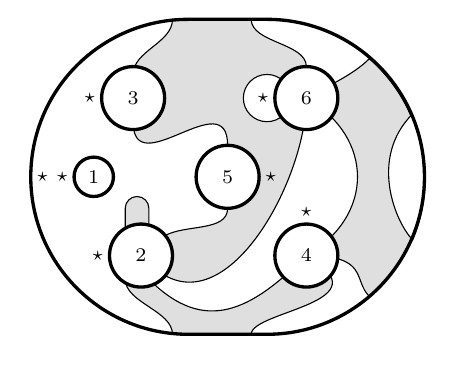
\begin{tikzpicture}[baseline = -.1cm]
	\filldraw[shaded] (.3,1.3) .. controls ++(90:.3cm) and ++(270:.3cm) .. (.8,2) -- 
		(1.8,2) .. controls ++(270:.3cm) and ++(90:.3cm) .. (2.5,1.4) --
		(2.5,1) .. controls ++(270:1cm) and ++(-30:1cm) .. (.7,-1.25) --
		(.7,-.75) .. controls ++(30:.3cm) and ++(270:.3cm) .. (1.5,-.4) -- 
		(1.5,.4) .. controls ++(90:.8cm) and ++(270:.8cm) .. (.3,.7);
	\filldraw[unshaded] (2,1) circle (.3cm);
	\filldraw[shaded] (.2,-.7) -- (.2,-.4) arc (180:0:.15cm) -- (.5,-.7);
	\filldraw[shaded]  (.2,-1.3) .. controls ++(270:.3cm) and ++(90:.3cm) .. (.8,-2) -- (1.8,-2)
		(1.8,-2) .. controls ++(90:.3cm) and ++(-30:1.2cm) .. (2.5,-1)
		.. controls ++(-135:1cm) and ++(-45:1cm) .. (.5,-1.3) -- (.2,-1.3);
	\filldraw[shaded] (2.5,1) .. controls ++(30:.3cm) and ++(-135:.3cm) .. (3.3,1.5)
		arc (49:-49:2cm)  .. controls ++(135:.3cm) and ++(0:.8cm) ..  (2.5,-1)
		.. controls ++(30:1cm) and ++(-30:1cm) .. (2.5,1);
	\filldraw[unshaded] (3.85,.8) .. controls ++(-135:.8cm) and ++(135:.3cm) .. (3.85,-.8) arc (-23:23:2cm);
%
	\draw[very thick] (-1,0) arc (180:90:2cm) -- (2,2) arc (90:-90:2cm) -- (1,-2) arc (-90:-180:2cm);
%	\halfcircle{}{(0,0)}{2}{2}{}
%
	\ncircle{unshaded}{(-.2,0)}{.25}{180}{\scriptsize{$1$}}
	\ncircle{unshaded}{(.3,1)}{.4}{180}{\scriptsize{$3$}}
	\ncircle{unshaded}{(.4,-1)}{.4}{180}{\scriptsize{$2$}}
	\ncircle{unshaded}{(2.5,1)}{.4}{180}{\scriptsize{$6$}}
	\ncircle{unshaded}{(1.5,0)}{.4}{0}{\scriptsize{$5$}}
	\ncircle{unshaded}{(2.5,-1)}{.4}{90}{\scriptsize{$4$}}
	\node at (-.85,0) {\scriptsize{$\star$}};
\end{tikzpicture}
$$
%
%
%\nn{todo: define $\widetilde{\cT}$ from $\cT$.}
%
%Now if $\cP_\bullet$ is a finite depth subfactor planar algebra and $\Phi : \cP_\bullet \hookrightarrow \cG_\bullet$ is a planar algebra embedding, then we may endow $\cM_\bullet$ with the structure of a connected right planar $\cP_\bullet$-module by defining 
%$$
%\rho_{k,n}(p_v m \otimes x) 
%:=
%\begin{tikzpicture}[baseline]
%\draw (0,-.7) -- (0,.7);
%\draw (1,-.7) -- (1,.7);
%\roundNbox{unshaded}{(-.8,0)}{.25}{0}{0}{$p_v$};
%\roundNbox{unshaded}{(0,0)}{.25}{0}{0}{$m$};
%\roundNbox{unshaded}{(1,0)}{.25}{.2}{.2}{$\Phi(x)$};
%\node at (0,-.9) {\tiny{$k$}};
%\node at (1,-.9) {\tiny{$n$}};
%\end{tikzpicture}
%\,.
%$$ 
\end{ex}



%%%%%%%%%%%%%%%%%%%%%%%%%%%%%%%%%%%%%%%%%%%%%%%%%%%%%%%
\subsection{Equivalence}


In this section, we sketch the proof of the following theorem.

\begin{thm*}[Theorem \ref{thm:ModuleEquivalence}]
%\label{thm:ModuleEquivalence}
Let $\cP_\bullet$ be a subfactor planar algebra corresponding to $(\cC, X)$ as above.
There is an equivalence between:
\begin{enumerate}[label={\rm(\arabic*)}]
\item
pivotal right $\cC$-module $\Cstar$ categories $(\cM,\Tr^\cM)$ with choice of simple basepoint $m = m\vartriangleleft 1_0$, and
\item
connected right planar modules $\cM_\bullet$ for $\cP_\bullet$.
\end{enumerate}
\end{thm*}

As an application, we get a classification of pivotal module $\Cstar$ categories for the 2-shaded Temperley-Lieb-Jones category with parameter $d$ in \S\ref{sec:TLJmodules}.

\nn{I expect Theorem \ref{thm:ModuleEquivalence} extends to an equivalence of categories.
What may be more relevant is the following theorem, which tells us when the underlying $\cC$-module $\Cstar$ categories are dagger equivalent.}

\begin{thm}
Suppose $M_\bullet$ and $N_\bullet$ are two cyclic right planar modules for $\cQ_\bullet$ and $(\cM, \Tr^\cM,m)$ and $(\cN, \Tr^\cN,n)$ are the corresponding cyclic pivotal right $\cC$-module $\Cstar$ categories under the bijective correspondence from Theorem \ref{thm:ModuleEquivalence}.
We have a dagger equivalence $\cM \cong \cN$ if and only if $N_\bullet$ can be obtained from $M_\bullet$ by a a shift and a compression as in \nn{}.
\end{thm}

%%%%%%%%%%%%%%%%%%%%%%%%%%%%%%%%%%%%%%%%%%%%%%%%%%%%%%%
\subsection{From pivotal module categories to planar modules}

Starting with the $2\times 2$ unitary multifusion category $\cC$ of projections of a finite depth subfactor planar algebra $\cQ_\bullet$ and an indecomposable right $\cC$-module category $\cM$ with distinguished simple object $m\in \cM$, we build a Markov tower and endow it with the structure of a right planar module for $\cQ_\bullet$.

%By a module over $Q_\bullet$, we mean a $\ast$-module category over the $\ast$-multitensor category $\cC$. Let $\cM$ be a cyclic left $\cC$-module category with generator $m$. 
%Since $\cM$ is indecomposable, we can take $m$ to be simple. 
By \cite{ostrik03}, there is an algebra $A$ internal to $\cC$ such that $\cM\cong\FreeMod_\cC(A)$, the category of free right $A$-modules internal to $\cC$, namely the $\cC$-valued internal $\End$ of $m$. 
Since $m$ is simple, 
$A$ is in fact a Q-system, % Q-system or $Q$-system?
as described in \cite[Rmk.~2.7]{ny17}.  
Each module in this category is of the form $X\otimes A$ for some $X\in\cC$. 
Each $X$ in $\cC$ is trivially a bimodule over the tensor unit $1_{0,+}\oplus1_{0,-}$, so each $X\in\Irr(\cC)$ is a module over either $1_{0,+}$ or $1_{0,-}$ on each side. 
We can therefore view $\cC$ as the $2$-category of bimodules over the algebra objects $1_{0,+}$ and $1_{0,-}$ and $\cM$ as the category of $1_{0,+}-A$ and $1_{0,-}-A$ bimodules. 
By \cite[Thm.~4.1]{ny17}, we can again obtain a $3\times 3$ unitary multifusion category $\widetilde{\cC}$ from the $2$-category of bimodules over the algebras $1_{0,+}$, $1_{0,-}$, and $A$, into which
$\cC$ has a monoidal dagger embedding and $\cM$ has a $\cC$-module dagger embedding.
Taking the full subcategory of objects which are preserved by tensoring by the appropriate components of the tensor unit allows us to recover a $2\times 2$ multifusion subcategory $\cC$ and a cyclic $\cC$-module $\cM$. 

%%%%%%%%%%%%%%%%%%%%%%%%%%%%%%%%%%%%%%%%%%%%%%%%%%%%%%%
%\section{Construction of the Planar Algebra Associated to a Module Category}
%\subsection{Constructing a Markov tower}

%Given a finite depth subfactor planar algebra $Q_{\bullet}$ and a module $\cM$ over $Q_{\bullet}$, let $\cC$ and $\widetilde{\cC}$ be the multifusion categories associated to $\cG$ and $\cM$, as described in section \ref{cattheory}. 

Let $1_{\widetilde{\cC}}= 1_0 \oplus 1_1 \oplus 1_2$ be the tensor unit in $\widetilde{\cC}$, indexed so that $\cC$ is the non-unital $2\times 2$ unitary multifusion subcategory of $\widetilde{\cC}$ with $1_\cC = 1_0\oplus 1_1$, and $\cM\cong\cC_{20}\oplus \cC_{21}$. Overall,
$$
\cM 
=
\begin{pmatrix}
\cC_{20} & \cC_{21} 
\end{pmatrix}
\qquad\qquad
\cC
=
\begin{pmatrix}
\cC_{00} & \cC_{01} 
\\
\cC_{10} & \cC_{11}
\end{pmatrix}
\subset
\begin{pmatrix}
\cC_{00} & \cC_{01} & \cC_{02}
\\
\cC_{10} & \cC_{11} & \cC_{12}
\\
\cC_{20} & \cC_{21} & \cC_{22}
\end{pmatrix}
=
\widetilde{\cC}
$$


\nn{redo below here -- get planar module from module category.}


Let $x\in \cC_{01}$ be the strand pictured below:
$$x=

\begin{tikzpicture}[baseline=-.1cm]
	\fill[white] (0,-.7) rectangle (-.7,-.7);
	\fill[shaded] (0,-.7) rectangle (.7,.7);
	\draw (0,-.7) -- (0,.7);

\end{tikzpicture}
\ \,\,\,\,\, \text{and,}\,\,\,\,\, \overline{x}=

\begin{tikzpicture}[baseline=-.1cm]
	\fill[white] (0,-.7) rectangle (.7,.7);
	\fill[shaded] (0,-.7) rectangle (-.7,.7);
	\draw[fill] (0,-.7) -- (0,.7);

\end{tikzpicture}
\,\,\,\,\, \text{so} \,\,\,\,\, x\otimes \overline{x} = 
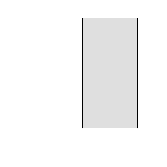
\begin{tikzpicture}[baseline=-.1cm]
	\fill[white] (0,-.7) rectangle (-.7,.7);
	\fill[shaded] (0,-.7) rectangle (.7,.7);
	\draw (0,-.7) -- (0,.7);
	\draw (.7,-.7) -- (.7,.7);

\end{tikzpicture}
$$
By construction, $x$ is a generating object for $\cC$. If we pick a simple object $m\in \cC_{20}$, since $\cM$ is indecomposable, we have that any object of $\cM$ is isomorphic to a direct summand of $m\otimes \xalt$ for some nonnegative integer $n$, where $$
x^{\text{alt}\otimes n}:=\underbrace{x\otimes \overline{x} \otimes x \otimes \cdots \otimes x^?}_{n \text{ tensorands}}\,,
$$ and $x^? = \overline x$ if $n$ is even and $x$ if $n$ is odd. We define $\xbaralt$ similarly.

We will construct a finite depth Markov tower of algebras from the action of $\cC$ on $\cM$ as follows. Set $M_n:=\End_{\widetilde{\cC}}(m\otimes \xalt)$. We can represent morphisms in $M_n$ as 
$$
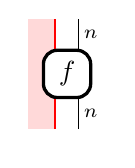
\begin{tikzpicture}[baseline=-.1cm]
	\fill[ctwoshading] (-.15,-.7) rectangle (-.5,.7);
	\draw[thick, red] (-.15,-.7) -- (-.15,.7);
	\draw (.15,-.7) -- (.15,.7);
	\roundNbox{unshaded}{(0,0)}{.3}{0}{0}{$f$}
	\node at (.3,.5) {\scriptsize{$n$}};
	\node at (.3,-.5) {\scriptsize{$n$}};
\end{tikzpicture}
$$
where the red strand represents $m$ and the $n$ represents $x^{\text{alt}\otimes n}$. We have a faithful tracial state $\tr_n:M_n\to \C$ given by
\begin{equation}\label{eq:TraceAn}
\tr_n(f) 
\,:=\, 
\frac{1}{\dim_{\widetilde{\cC}}(m)\dim_{\widetilde{\cC}}(x)^n}\cdot\tr_{\widetilde{\cC}}(f)
\,=\,
\frac{1}{\dim_{\widetilde{\cC}}(m)}\cdot
\frac{1}{d^n}
\cdot
\left(
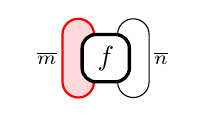
\begin{tikzpicture}[baseline=-.1cm, rotate=90]
	\filldraw[thick, red, ctwoshading] (-.3,.15) arc (270:90:.2cm) -- (.3,.55) arc (90:-90:.2cm);
	\draw (-.3,-.15) arc (90:270:.2cm) -- (.3,-.55) arc (-90:90:.2cm);
	\roundNbox{unshaded}{(0,0)}{.3}{0}{0}{$f$}
%	\node at (-.7,-.35) {\scriptsize{$n$}};
	\node at (0,-.7) {\scriptsize{$\overline{n}$}};
	\node at (0,.75) {\scriptsize{$\overline{m}$}};
%	\node at (.7,.35) {\scriptsize{$m$}};
\end{tikzpicture}
\right)
\end{equation}
Where $n$ and $\overline{n}$ represent $\xalt$ and $\xbaralt$, respectively. 
This makes each $M_n$ a finite dimensional von Neumann algebra.

\nn{$A_n \to M_n$ by convention for Markov towers. decide whether to keep next remark environment or make this a footnote.}

\begin{rem}
	The trace can be identified with a complex scalar because $\overline{m}\otimes m\in\cC_{00}$, the red cup $1\to\overline{m}\otimes m$ and cap $\overline{m}\otimes m\to 1$ factor through the simple summand $1_0$. Since $1_0\otimes 1\cong 1_0$, the trace is a member of the $1$-dimensional algebra $\End_{\widetilde{\cC}}(1_0)\subseteq\End_{\widetilde{\cC}}(1)$. 
\end{rem}

%We also have a natural tracial inclusion $A_n \rightarrow A_{n+1}$ % such that the trace restricts ($tr_{n+1}|_{A_n}=tr_n$):
%\begin{equation}\label{eq:Inclusion}
%\begin{tikzpicture}[baseline=-.1cm]
%	\fill[ctwoshading] (-.15,-.7) rectangle (-.5,.7);
%	\draw[thick, red] (-.15,-.7) -- (-.15,.7);
%	\draw (.15,-.7) -- (.15,.7);
%	\roundNbox{unshaded}{(0,0)}{.3}{0}{0}{$f$}
%	\node at (.3,.5) {\scriptsize{$n$}};
%	\node at (.3,-.5) {\scriptsize{$n$}};
%\end{tikzpicture}
%\mapsto
%\begin{tikzpicture}[baseline=-.1cm]
%	\fill[ctwoshading] (-.15,-.7) rectangle (-.5,.7);
%	\draw[thick, red] (-.15,-.7) -- (-.15,.7);
%	\draw (.15,-.7) -- (.15,.7);
%	\draw (.45,-.7) -- (.45,.7);
%	\roundNbox{unshaded}{(0,0)}{.3}{0}{0}{$f$}
%	\node at (.15,.9) {\scriptsize{$n$}};
%	\node at (.15,-.9) {\scriptsize{$n$}};
%	\node at (.6,0) {\scriptsize{$1$}};
%\end{tikzpicture}
%\end{equation}
%and a trace preserving conditional expectation $E_n:A_n\rightarrow A_{n-1}$, 
%\begin{equation}\label{eq:ConditionalExpectationAn}
%\begin{tikzpicture}[baseline=-.1cm]
%	\fill[ctwoshading] (-.15,-.7) rectangle (-.5,.7);
%	\draw[thick, red] (-.15,-.7) -- (-.15,.7);
%	\draw (.15,-.7) -- (.15,.7);
%	\roundNbox{unshaded}{(0,0)}{.3}{0}{0}{$f$}
%	\node at (.3,.5) {\scriptsize{$n$}};
%	\node at (.3,-.5) {\scriptsize{$n$}};
%\end{tikzpicture}
%\mapsto\,
%\frac{1}{d}
%\cdot
%\left(\,\,
%\begin{tikzpicture}[baseline=-.1cm]
%	\fill[ctwoshading] (-.15,-.7) rectangle (-.5,.7);
%	\draw[thick, red] (-.15,-.7) -- (-.15,.7);
%	\draw (0,-.7) -- (0,.7);
%	\draw (.15,.3) arc (180:0:.15cm) -- (.45,-.3) arc (0:-180:.15cm);
%	\roundNbox{unshaded}{(0,0)}{.3}{0}{0}{$f$}
%	\node at (.4,.6) {\scriptsize{$n-1$}};
%	\node at (.4,-.6) {\scriptsize{$n-1$}};
%	\node at (.6,0) {\scriptsize{$1$}};
%\end{tikzpicture}
%\right)
%\end{equation}
%left inverse to the inclusion.
%
%Here, $d:=\dim_{\widetilde{\cC}}(x)=\dim_{\widetilde{\cC}}(\overline{x})$ the value of a closed loop appearing in the diagram. % There must be a better word for this. Maybe we should also remark why these are equal? In response: Emily peter's uses the term closed circles (on page 7 of her thesis), if that's the woridng you mean, and the equality follows from sphericality, maybe we should this should probably be in the preliminary discussion of the paragroup and the constructed multifusion category
%Given the previously defined inclusion and that multiplication is given by vertical stacking of diagrams, it's clear that $E_n$ is $A_{n-1}$ bilinear. Similarly, we have that $tr_n=tr_{n-1} \circ E_n$.
%
%Finally, the Jones projections for each inclusion $A_{n}\subset A_{n+1}$ are given by
%\begin{equation}\label{eq:JonesProjections}
%e_n
%:=
%\frac1d\cdot
%\left(\,\,
%\begin{tikzpicture}[baseline=-.1cm]
%	\fill[ctwoshading] (-.3,-.7) rectangle (-.6,.7);
%	\draw[thick, red] (-.3,-.7) -- (-.3,.7);
%	\draw (-.1,-.7) -- (-.1,.7);
%	\draw (.1,-.7) -- (.1,-.4) arc (180:0:.15cm) -- (.4,-.7);
%	\draw (.1,.7) -- (.1,.4) arc (-180:0:.15cm) -- (.4,.7);
%%	\node at (-.1,-1) {\scriptsize{$n-1$}};
%	\node at (.3,0) {\scriptsize{$n-1$}};
%	\node at (.6,.5) {\scriptsize{$1$}};
%	\node at (.6,-.5) {\scriptsize{$1$}};
%\end{tikzpicture}
%\right)
%\in
%A_{n+1}.
%\end{equation}
%where the $n-1$ indicates $n-1$ vertical strands with appropriate shading to the right of the red strand. The Temperley-Lieb- % strange editor enforced wordwrap from here. lint?
%Jones relations follow immediately from the definition and the fact that closed loops count for a factor of $d$. Similarly, 
%for any $x\in A_n$ we have $e_nxe_n=E_n(x)e_n$. Clearly, $E_{n+1}(e_n)=d^{-2}\id_{m \otimes \xalt}$. Finally, the pull 
%down condition holds, as for each $x\in A_{n+1}$, we have that $d^2 E_{n+1}(xe_n)e_n=xe_n$. Equivalently, $A_{n} e_n A_n$ is a 
%two-sided ideal in $A_{n+1}$. Thus, the tower algebras given by the $A_n$ is indeed a Markov tower. 
% 
% 
%\begin{prop}
%The Markov tower of von Neumann Algebras $\left(A_n, tr_n\right)_{n\geq 0}$ is finite depth.
%\end{prop}
%
%\begin{proof}
%	When $n$ is even, we have:
%	\[m\otimes \xalt \cong \bigoplus\limits_{Y\in\Irr(\cC_{20})}\left(n_YY\right) \]
% For some nonnegative integers $n_Y$. Therefore, 
%	\[\End_{\widetilde{\cC}}\left(m\otimes\xalt\right)\cong \bigoplus\limits_{Y\in \Irr(\cC_{20})}\End_{\widetilde{\cC}}\left(n_Y Y\right) \]
%	The case when $n$ is odd is similar. This means that the Bratteli diagram for $A_n\subseteq A_{n+1}$ has at most $|\Irr(\cC_{20})|+|\Irr(\cC_{21})|$ vertices, so the principal graph must be finite. 
%\end{proof}
%
%\begin{thm}
%The principal graph obtained from the Markov tower $\left(A_n, tr_n\right)_{n\geq 0}$ is independent of the choice of $m$, and is in fact isomorphic to the fusion graph for the action of $x$ on $\cM$.
%\end{thm}
%
%\begin{proof}
%Because $x$ generates $\cC$ and $\cM$ is cyclic, we can assume that every simple object in $\cM$ is a direct summand of $m\otimes \xalt $. Essentially, our result from the fact that subsequent in inclusions $A_k\subseteq A_{k+1}$ are given by tensoring $\id_x$ and $\id_{\overline{x}}$, so they are determined entirely by the fusion rules.
%
%First, recall that for a finite depth Markov tower, the principal graph is canonically isomorphic to the Bratteli for the inclusion $A_n\subseteq A_{n+1}$ for $n$ large enough by \ref{BratteliPrincipal}. So, it suffices to show this Bratteli diagram is isomorphic to the fusion graph for $\cM$. Furthermore if $n$ is such that $A_n\subseteq A_{n+1}\subseteq A_{n+2}$ is standard then for $k\geq n$ the Bratteli diagram for $A_{k}\subseteq A_{k+1}$ is isomorphic to the Bratteli diagram for $A_n\subseteq A_{n+1}$, so without loss of generality, we may assume that $n$ is even.
%
%Let the non-negative integers $p_{Z,Y}$ be defined by the following equation:
%	\[Y\otimes x\cong\bigoplus\limits_{\Irr(\cC_{21})}\left(p_{Z,Y}Z\right)\]
%These coefficients are exactly the coefficients for the adjacency matrix of the fusion graph for $x$ acting on $\cM$.
%
%Recall that
%$$A_n=\End_{\widetilde{\cC}}\left(m\otimes\xalt\right)\cong \bigoplus\limits_{\Irr(\cC_{20})}\End_{\widetilde{\cC}}\left(n_Y Y\right)$$
%where 
%$$m \otimes \xalt \cong \bigoplus\limits_{\Irr(\cC_{20})}\left(n_YY\right)$$
%	Note that we may choose $n$ such that each $n_Y$ is strictly positive, as there is some $n$ such that $\bigoplus\limits_{\Irr(\cC_{20})}Y$ is isomorphic to a direct summand of $m\otimes \xalt$. (In fact, the first $n$ where this happens is exactly when the Markov tower achieves depth.) % Strictly speaking, this is not true, because the Markov tower may first achieve depth when $n$ is odd. But going into that may not clarify the proof. 
%
%The inclusion of $A_n \hookrightarrow A_{n+1}$ is given by $\phi \mapsto \phi \otimes \id_{x}$. Each $\phi \in A_n$ is uniquely defined as a direct sum \[\bigoplus\limits_{\Irr(\cC_{20})}\phi_Y\]
%where each $\phi_Y \in \End_{\widetilde{\cC}}\left(n_YY\right)$. Then, distributing tensor products over the sum, we may write $\phi$ as 
%	\[\bigoplus_{\Irr(\cC_{20})}\left(\phi_Y \otimes \id_{x}\right)\]
%But then:
%	\[\phi_Y \otimes \id_{x} \in \End_{\widetilde{\cC}}\left(n_Y Y \otimes x\right)\cong \bigoplus\limits_{\Irr({\cC}_{21})} \End_{\widetilde{\cC}}\left( p_{Z,Y} n_Y Z\right)\]
%Since all $n_j\neq 0$ and the inclusion is unital, it is clear that $p_{Z,Y}$ gives the coefficients for the Bratteli diagram.
%\end{proof}
%
%\nn{endow this markov tower with the structure of a right planar module for $\cQ_\bullet$.}



%%%%%%%%%%%%%%%%%%%%%%%%%%%%%%%%%%%%%%%%%%%%%%%%%%%%%%%
\subsection{From planar modules to pivotal module categories}

\nn{
First define action of $\cC_0$, whose objects are alternating tensor powers of $X$ and $\overline{X}$ and whose morphisms are the box spaces.
Define action on $\cM_0$.
Then idempotent complete to get action of $\cC$ on $\cM$.
\\
\\
Define $[2n] \vartriangleleft X^{\otimes \text{alt}k} := [2n+k]$.
\\
\\
Define $f \vartriangleleft g$ similar to tensor product in projection category $\cC$, which has 4 distinct definitions based on source and target of $f$ and $g$ (which is larger).
Taking daggers reduces to 2 cases.
}





\nn{TODO: When $M_\bullet$ is a cyclic right planar module for $\cQ_\bullet$ with projection categories $\cM$ and $\cC$ respectively, endow $\cM$ with the structure of a cyclic right $\cC$-module $\Cstar$ category.}


%%%%%%%%%%%%%%%%%%%%%%%%%%%%%%%%%%%%%%%%%%%%%%%%%%%%%%%
%%%%%%%%%%%%%%%%%%%%%%%%%%%%%%%%%%%%%%%%%%%%%%%%%%%%%%%
%%%%%%%%%%%%%%%%%%%%%%%%%%%%%%%%%%%%%%%%%%%%%%%%%%%%%%%
\section{Markov towers and their projection categories} 
\label{sec:MarkovTowers}

\nn{edit now.}

We begin the article by defining the notion of a \emph{Markov tower} of finite dimensional tracial von Neumann algebras and studying its elementary properties.
One should think of the definition of a Markov tower as obtained from the definition of Popa's $\lambda$-\emph{sequences of commuting squares} from \cite{MR1334479} and forgetting one of the towers.
This is analogous to the way one defines a module for an algebraic object by replacing one argument of the algebraic operation with an element from the module.
In \S\ref{sec:TLJmodules} below, we will see that Markov towers are exactly a $\lambda$-lattice approach to pivotal Temperley-Lieb-Jones module categories.

%%%%%%%%%%%%%%%%%%%%%%%%%%%%%%%%%%%%%%%%%%%%%%%%%%%%%%%
\subsection{Markov towers and their elementary properties}
\label{sec:MarkovTowersAndElementaryProperties}

The towers of algebras analog of a module category is played by the role of a \emph{Markov tower}.

\begin{defn}
A \emph{Markov tower} $M_\bullet = (M_n, \tr_n, e_{n+1})_{n\geq 0}$ consists of a sequence $(M_n, \tr_n)_{n\geq 0}$ of finite dimensional von Neumann algebras, such that $M_n$ is unitally included in $M_{n_1}$, each $M_n$ has a faithful normal tracial states such that $\tr_{n+1}|_{M_n} = \tr_n$ for all $n\geq 0$, and there is a sequence of \emph{Jones projections} $e_n \in M_{n+1}$ for all $n\geq 1$, such that:
\begin{enumerate}[label={\rm(M\arabic*)}]
\item
\label{eq:MarkovJonesProjections}
The projections $(e_n)$ satisfy the Temperley-Lieb-Jones relations:
\begin{enumerate}[label={\rm(\alph*)}]
\item
$e_i^2 = e_i = e_i^*$ for all $i$,
\item
$e_i e_j = e_j e_i$ for $|i-j|>1$, and
\item
there is a fixed constant $d>0$ called the \emph{modulus} such that $e_{i} e_{i\pm 1} e_i = d^{-2} e_i$ for all $i$.
\end{enumerate}
\item
\label{eq:MarkovImplement}
For all $x\in M_n$, $e_n x e_n = E_n(x)e_n$, where $E_n: M_n \to M_{n-1}$ is the canonical faithful trace-preserving conditional expectation.
\item
\label{eq:MarkovIndex}
For all $n\geq 1$, $E_{n+1}(e_n) = d^{-2}$.
\item
\label{eq:MarkovPullDown}
(pull down)
For all $n\geq 1$, $M_{n+1}e_n = M_n e_n$.

\end{enumerate}
\end{defn}

\begin{rem}
One should think of the following definition as obtained from Popa's definition of \emph{$\lambda$-sequence} \cite{MR1334479} and removing one of the two sequences of algebras, together with the commuting square condition.
Compare the existence of Jones projections \ref{eq:MarkovJonesProjections} and \ref{eq:MarkovImplement} with (1.3.2), and \ref{eq:MarkovIndex} and \ref{eq:MarkovPullDown} with (1.3.3') from \cite{MR1334479} respectively.)
\end{rem}


\begin{rem}\label{pulldowniff}
$M_n e_n M_n$ is a 2-sided ideal in $M_{n+1}$ for all $n\geq 1$ if and only if the pull down condition holds. Indeed, if the pull down condition holds, then $M_{n+1} M_n e_n M_n \subseteq M_{n+1} e_n M_n = M_n e_n M_n$; the same argument holds on the right by first taking adjoints. Conversely, if $M_n e_n M_n$ is a 2-sided ideal, then $M_{n+1} e_n = (M_{n+1} e_n)e_n \subseteq (M_n e_n M_n) e_n = M_n e_n$.
\end{rem}




\begin{prop}\label{prop:ElementaryMarkov} A Markov tower satisfies the following elementary properties for $n\geq 1$.
\begin{enumerate}[label={\rm(EP\arabic*)}]
\item
\label{EP:Injective}
The map $M_{n}\ni y\mapsto ye_n \in M_{n+1}$ is injective.

\item
\label{EP:UniquePullDown}
For all $x\in M_{n+1}$, $d^{2}E_{n+1}(x e_n)$ is the unique element $y\in M_n$ such that $x e_n = ye_n$ \cite[Lem.~1.2]{MR860811}.

\item
\label{EP:MarkovTraces}
The traces $\tr_{n+1}$ satisfy the following \emph{Markov property} with respect to $M_n$ and $e_n$: for all $x\in M_n$, $\tr_{n+1}(xe_n) = d^{-2} \tr_n(x)$.

\item
\label{EP:CompressM_{n+1}}
$e_n M_{n+1}e_n = M_{n-1}e_n$.

\item
\label{EP:2SidedIdeal}
$X_{n+1}:=M_n e_n M_n$ is a 2-sided ideal of $M_{n+1}$, and thus $M_{n+1}$ splits as a direct sum of von Neumann algebras $X_{n+1}\oplus Y_{n+1}$.
(In \cite[Thm.~4.1.4 and Thm.~4.6.3]{MR999799}, $Y_{n+1}$ is the so-called `new stuff'.)
By convention, we define $Y_0 = M_0$ and $Y_1 = M_1$, so that $X_0 = (0)$ and $X_1 = (0)$.

\item
\label{EP:BasicContruction}
The map $ae_n b\mapsto ap_n b$ gives a $*$-isomorphism from $X_{n+1}=M_n e_n M_n$ to $\langle M_n , p_n\rangle=M_np_nM_n$, the Jones basic construction of $M_{n-1} \subseteq M_n$ acting on $L^2(M_n,\tr_n)$.

\item
\label{EP:OtherMarkovDef}
Under the isomorphism $X_{n+1} \cong M_n p_n M_n$, the canonical non-normalized trace $\Tr_{n+1}$ on the Jones basic construction algebra $M_np_nM_n$ satisfying $\Tr_{n+1}(ap_nb) = \tr_n(ab)$ for $a,b\in M_n$ equals $d^2 \tr_{n+1}|_{X_{n+1}}$.

\item
\label{EP:NewStuff}
If $y\in Y_{n+1}$ and $x\in X_{n}$, then $yx = 0$ in $M_{n+1}$.
Hence $E_{n+1}(Y_{n+1}) \subseteq Y_{n}$.
(``The new stuff comes only from the old new stuff" \cite{MR999799}.)

\item
\label{EP:FiniteDepth}
If $Y_n =(0)$, then $Y_{k} = (0)$ for all $k\geq n$.

\end{enumerate}
\end{prop}

\begin{proof} 
\mbox{}
\begin{enumerate}[label={\rm(EP\arabic*)}]
\item
By \ref{eq:MarkovIndex}, $d^2E_{n+1}(ye_n) = y $, so the proposed map has a left inverse.

\item
This follows directly from \ref{eq:MarkovPullDown} and \ref{EP:Injective}.

\item
By \ref{eq:MarkovIndex}, for $x\in M_n$, we have $\tr_{n+1}(xe_n) = \tr_n(E_{n+1}(xe_n)) = \tr_n(x E_{n+1}(e_n)) = d^{-2} \tr_n(x)$.
%, since $E_{n+1}(e_n) = d^{-2}$.

\item
By \ref{eq:MarkovPullDown}, $e_n M_{n+1} e_n= e_nM_n e_n$.
By \ref{eq:MarkovImplement}, $e_n M_n e_n = M_{n-1}e_n$.

\item
That $M_ne_nM_n$ is a 2-sided ideal is equivalent to \ref{eq:MarkovPullDown} as in Remark \ref{pulldowniff}.

\item
It suffices to show the map is injective, which also shows it is well-defined. % This was written here, but I can't make sense of it. 
%First, we check that the map $\phi:ae_nb\to ap_nb$ is injective. 
Suppose $\sum a_i p_n b_i = 0$.
Then for all $a,b\in M_n$, we have $0=p_na\left(\sum a_i p_n b_i\right) bp_n = \sum E_{n}(aa_i)E_n(b_ib)p_n$, and therefore $\sum E_{n}(aa_i)E_n(b_ib) = 0$ as $M_n \ni x\mapsto xp_n \in \langle M_n, p_n\rangle$ is injective by \ref{EP:Injective} applied to the Jones tower for $M_{n-1} \subset (M_n,\tr_n)$, which is a Markov tower.
Hence 
$$
0 = \sum E_{n}(aa_i)E_n(b_ib)e_n = e_na\left(\sum a_i e_n b_i\right) be_n
$$ 
for all $a,b\in M_n$, and thus $\sum a_i e_n b_i = 0$, so the map is injective. 

%To show that $\phi$ is well-defined, we may reverse the above argument, using \ref{EP:Injective}. 
%		It is clear that $\phi$ is surjective. 

\item
For $a,b\in M_n$, by \ref{EP:MarkovTraces}, 
$\Tr_{n+1}(ap_n b) = \tr_n(ab) = \tr_n(ba) = d^2\tr_{n+1}(bae_n) = d^2 \tr_{n+1}(ae_n b)$.

\item
Since $X_0 = (0)$ and $X_1 = (0)$ by definition, we may assume $n\geq 2$.
As in the proof of \cite[Thm.~4.6.3.vi]{MR999799}, we may assume $y$ is a central projection in $M_{n+1}$ such that $y e_{n} = 0$.
Then for all $ae_{n-1} b \in X_n$, by \ref{eq:MarkovJonesProjections}, $y ae_{n-1} b = d^2 yae_{n-1} e_{n}e_{n-1} b = d^2 ae_{n-1} ye_{n} e_{n-1} b = 0$.
The final claim follows from $z_{n}E_{n+1}(y) = E_{n+1}(z_n y)= 0$ where $z_n$ is the central support of $e_{n-1}$ in $M_n$.

\item
This follows immediately from \ref{EP:NewStuff}.
\qedhere

\end{enumerate}
\end{proof}

\begin{rem}
\nn{we stick to finite dimensions, but what came above in this section works if the $(M_n,\tr_n)$ are arbitrary tracial von Neumann algebras.
We stick to finite dimensions because we want a principal graph; this notion would need to be generalized to an infinite setting...}
\end{rem}


Notice that by \ref{EP:BasicContruction}, the Bratteli diagram for the inclusion $M_{n}\subset M_{n+1}$ consists of the reflection of the Bratteli diagram for the inclusion $M_{n-1} \subset M_n$, together with possibly some new edges and vertices corresponding to simple summands of $Y_{n+1}$. 
By \ref{EP:NewStuff}, the new vertices at level $n+1$ only connect to the vertices that were new at level $n$. This leads to the following definition:

\begin{defn}
The \emph{principal graph} of the Markov tower $(M_n,\tr_n, e_{n+1})$ consists of the \emph{new} vertices at every level $n$ of the Bratteli diagram, together with all the edges connecting them.

A Markov tower is said to have \emph{finite depth} if the principal graph is finite.
\end{defn}


It follows that a Markov tower has finite depth if and only if there is $n\in \bbN$ such that $Y_n = (0)$, as in \ref{EP:FiniteDepth}. 
Let $(M_n)$ be a Markov tower with finite depth, and take the minimal integer $n\in \bbN$ such that $Y_n=(0)$. 
Now notice that for $k<n$ the Bratteli diagram of $M_k\subseteq M_{k+1}$ is the Bratteli diagram of $M_{k-1}\subseteq M_{k}$ reflected upwards along with additional edges which are part of the principal graph. 
Because of this and the fact that the Bratteli diagram for $M_0\subseteq M_1$ is part of the principal graph we can ``unravel" the Bratteli diagram for $M_{n}\subseteq M_{n+1}$ to obtain the principal graph for the Markov tower $(M_n,\tr_n,e_{n+1})$.

\begin{fact}\label{BratteliPrincipal}
	If a Markov tower $(M_n)$ has finite depth and $n\in \bbN$ is such that $Y_n=(0)$, then for $k\geq n$, there is a canonical graph isomorphism between the principal graph of $(M_n)$ and the Bratteli diagram for $M_{k}\subseteq M_{k+1}$.
\end{fact}

%%%%%%%%%%%%%%%%%%%%%%%%%%%%%%%%%%%%%%%%%%%%%%%%%%%%%%%
\subsection{Examples of Markov towers}

\nn{talk about planar modules here.}


\begin{ex}
The Temperley-Lieb-Jones algebras of modulus $d\geq 2$ with the usual Jones projections and Markov traces form a Markov tower with principal graph $A_{\infty}$.
\end{ex}


\begin{ex}
\nn{take a $\cC$-module and get a markov tower.
This is the same as taking a planar module and getting a markov tower.}
\end{ex}

\nn{edit:}

\nn{adapt for planar modules.}

\begin{lem}
Suppose $\cP_\bullet$ is a finite depth subfactor planar algebra and $\cM_\bullet$ is a right planar module for $\cP_\bullet$.
Then the associated Markov tower $M_\bullet$ has finite depth, with $\operatorname{depth}(M_\bullet) \leq \operatorname{depth}(\cP_\bullet)$.
\end{lem}
\begin{proof}
Let $r$ be minimal such that $\cP_{r+1,+} = \cP_{r,+} e_{r,+}\cP_{r,+}$, and let $\{b\}$ be a Pimsner-Popa basis for $\cP_{r+1,+}$ over $\cP_{r,+}$ so that $\sum_b b e_{r,+} b^* = 1_{\cP_{r+1,+}}$.
Since $1_{M_{r+1}} = 1_{\cP_{r+1,+}}$ \nn{picture for this?}, we have that
%Then 
%\nn{pictures below?}
%\begin{align*}
%1_{M_{r+1}}
%&=
%1_{\cP_{r+1,+}}
%=
%\sum_b
%b(e_{r,+})b^*
%\\&=
%=
%\sum_b
%b
%\rho^{0}_{r+1}(e_{r,+})
%\rho^{0}_{r+1}(b^*)
%d^{-1}
%\sum_b
%\rho_{0,r+1}\left(
%1_{M_0}\otimes
%\begin{tikzpicture}[baseline=-.1cm]
%	\draw (-.2,-1) -- (-.2,1);
%	\draw (.2,1) -- (.2,.25) arc (-180:0:.2cm) -- (.6,1);
%	\draw (.2,-1) -- (.2,-.25) arc (180:0:.2cm) -- (.6,-1);
%	\roundNbox{unshaded}{(0,.5)}{.25}{.1}{.1}{$b$}
%	\roundNbox{unshaded}{(0,-.5)}{.25}{.1}{.1}{$b^*$}
%	\node at (-.35,-.9) {\scriptsize{$r$}};
%	\node at (-.35,0) {\scriptsize{$r$}};
%	\node at (-.35,.9) {\scriptsize{$r$}};
%\end{tikzpicture}
%\,\,\,
%\right)
%\\&=
%=
%\sum_b
%\rho^{0}_{r}(b)
%p_r
%\rho^{0}_{r}(b^*).
%\end{align*}
%Hence 
$\{b\}$ is a Pimsner-Popa basis for $M_{r+1}$ over $M_r$.
Hence $M_\bullet$ has finite depth by \ref{EP:FiniteDepth}.
The last claim follows immediately.
\end{proof}


\nn{move later:}
\begin{ex}
\nn{define strongly markov inclusion.}

Given a strongly Markov inclusion of tracial von Neumann algebras $A_0\subset (A_1, \tr_1)$, its Jones tower $(A_n, \tr_n, e_{n+1})$ is a Markov tower.
\nn{decide whether Markov tower should mean finite dimensional.}

Taking the relative commutant with $A_0$, we get a Markov tower of \emph{finite dimensional} von Neumann algebras $(A_0'\cap A_n , \tr_n|_{A_0'\cap A_n} , e_{n+1})$.
Similarly, $(A_1'\cap A_{n+1} , \tr_{n+1}|_{A_1'\cap A_{n+1}} , e_{n+2})$ is a Markov tower of finite dimensional von Neumann algebras.
\end{ex}

%%%%%%%%%%%%%%%%%%%%%%%%%%%%%%%%%%%%%%%%%%%%%%%%%%%%%%%
\subsection{Operations on Markov towers to produce new Markov towers}
\label{sec:OperationsOnMarkovTowers}

In this section, we describe various operations on a Markov tower $M_\bullet = (M_n, \tr_n, e_{n+1})_{n\geq 0}$ which yield new Markov towers.
We begin with shifting and compressing the tower.
We then study the multistep tower.
For each of these operations, we discuss how the principal graph changes. 
\nn{TODO!}

We omit the proof of the following straightforward proposition.

\begin{prop}[Shifting a Markov tower]
\label{prop:ShiftMarkovTower}
Suppose $(M_n, \tr_n, e_{n+1})$ is a Markov tower.
For any $k\geq 1$, $(M_{n+k}, \tr_{n+k}, e_{n+k+1})$ is also a Markov tower.
\end{prop}

%Similar to the discussion in \S\ref{sec:CompressionIso}, 
Given a Markov tower $(M_n,\tr_n, e_{n+1})$, we obtain another Markov tower by compression by a non-zero projection $p\in P(M_0)$.
First, for all $n\geq 0$, we define a faithful trace $\tr_n^p$ on $pM_n p$ by
\begin{equation}
\label{eq:CompressedTrace}
\tr^p_n(x) := \tr_n(p)^{-1}\tr_n(pxp).
\end{equation}
It is straightforward to verify that the unique trace-preserving conditional expectation is given by 
\begin{equation}
\label{eq:CompressedConditionalExpectation}
E^p_n : pM_np \to pM_{n-1}p
\qquad
\qquad
E^p_n(pxp) := E_n(pxp) = pE_n(x)p
\end{equation}
Notice that since $[e_n,p] = 0$ for all $n\in \bbN$, we have for all $pxp \in pM_n p$, we have 
\begin{equation}
\label{eq:CompressionImplementsConditionalExpectation}
e_np (pxp) e_np = p e_nxe_np = pE_n(x)e_np = E_n^p(pxp)e_np,
\end{equation}
so the conditional expectation is implemented by $e_np$.

\begin{prop}
Suppose $(M_n,\tr_n, e_{n+1})$ is a Markov tower of finite dimensional von Neumann algebras and $p\in P(M_0)$ is a nonzero projection.
Then $(pM_np, \tr_n^p, pe_{n+1})$ is a Markov tower, where $\tr_n^p$ is defined as in \eqref{eq:CompressedTrace}.
\end{prop}
\begin{proof}
First, it is easy to see that the projections $(pe_n)_{n\geq 1}$ satisfy the Temperley-Lieb-Jones relations \ref{eq:MarkovJonesProjections}, since $[e_n,p]=0$ for all $n\geq 0$.
That $pe_n$ implements the trace-preserving conditional expectation $pM_np \to pM_{n-1}p$ as in \ref{eq:MarkovImplement} was shown above in \eqref{eq:CompressionImplementsConditionalExpectation}.
Using \eqref{eq:CompressedConditionalExpectation}, this immediately implies that $E_{n+1}^p(pe_n) = pE_{n+1}(e_n) = d^{-2}p = d^{-2} 1_{M_n}$, so \ref{eq:MarkovIndex} holds.
Finally, for all $n\geq 1$, $pM_{n+1}p (pe_n) = pM_{n+1}e_np = pM_ne_np = pM_npe_n$, so we have \ref{eq:MarkovPullDown}.
\end{proof}

\begin{nota}
\label{nota:TLJK Diagrams}
We will make heavy use of the string diagrammatic representation of Temperley-Lieb-Jones diagrams.
Ordinarily, for subfactors and planar algebras, Kauffman diagrams \cite{MR899057} are drawn with strings going from \emph{bottom to top}. 
We put the number $k$ above or next to a strand to denote a bundle of $k$ parallel strands, and the label is omitted for single strands.
For example, the generators $E_i = de_i$ are represented by
$$
E_i
=
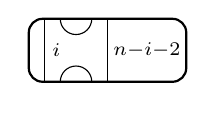
\begin{tikzpicture}[baseline = .3cm]
	\draw[thick, rounded corners = 5pt] (0,0) rectangle (2,.8);
	\draw (.2,0) -- (.2,.8);
	\draw (1,0) -- (1,.8);
	\draw (.4,.8) arc (-180:0:.2cm);
	\draw (.4,0) arc (180:0:.2cm);
%	\node at (.4,1) {\scriptsize{$1$}};
%	\node at (.4,-.2) {\scriptsize{$1$}};
	\node at (.35,.4) {\scriptsize{$i$}};
	\node at (1.5,.4) {\scriptsize{$n{-}i{-}2$}};
\end{tikzpicture}\,.
$$
Of particular importance will be the \emph{cabled/multi-step} Jones projections from \cite{MR965748} which were of importance in \cite{MR1424954,MR2812459}:
\begin{align*}
f^{j+k}_j
&:=
d^{k(k-1)}(e_{j+k}e_{j+k-1}\cdots e_{j+1})(e_{j+k+1}e_{j+k}\cdots e_{j+2})\cdots(e_{j+2k-1}e_{j+2k-2}\cdots e_{j+k})
\\
F^{j+k}_j
&:=
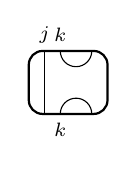
\begin{tikzpicture}[baseline = .3cm]
	\draw[thick, rounded corners = 5pt] (0,0) rectangle (1,.8);
	\draw (.2,0) -- (.2,.8);
	\draw (.4,.8) arc (-180:0:.2cm);
	\draw (.4,0) arc (180:0:.2cm);
	\node at (.4,1) {\scriptsize{$k$}};
	\node at (.4,-.2) {\scriptsize{$k$}};
	\node at (.2,1) {\scriptsize{$j$}};
\end{tikzpicture}
=
d^k f^{j+k}_j.
\end{align*}
We record the following relation for later use:
\begin{equation}
\label{eq:MultistepRelation}
f^{j+k}_j
=
d^{k(k-1)}(e_{j+k}e_{j+k+1}\cdots e_{j+2k-2}e_{j+2k-1})
\cdot\,
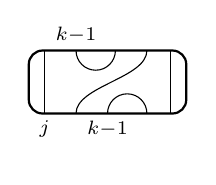
\begin{tikzpicture}[baseline = .3cm]
	\draw[thick, rounded corners = 5pt] (0,0) rectangle (2,.8);
	\draw (.2,0) -- (.2,.8);
	\draw (1.8,0) -- (1.8,.8);
	\draw (.6,.8) arc (-180:0:.25cm);
%	\draw (1.5,.8) arc (-180:0:.15cm);
	\draw (.6,0)  .. controls ++(90:.35cm) and ++(270:.35cm) .. (1.5,.8);
	\draw (1,0) arc (180:0:.25cm);
%	\node at (.7,-.2) {\scriptsize{$1$}};
%	\node at (1.8,1) {\scriptsize{$1$}};
%	\node at (2,-.2) {\scriptsize{$1$}};
	\node at (.6,1) {\scriptsize{$k{-}1$}};
	\node at (1,-.2) {\scriptsize{$k{-}1$}};
	\node at (.2,-.2) {\scriptsize{$j$}};
\end{tikzpicture}
\end{equation}

Now suppose we fix $j\geq 0$ and $k\geq 1$.
For $n\in \bbN$, define the $k$-cabled Jones projections
$
g_n := f^{j+nk}_{j+(n-1)k}
$.
It is straightforward to verify using Kauffman's diagrammatic calculus for Temperley-Lieb-Jones algebras that the projections $(g_n)_{n\in \bbN}$ satisfy the Temperley-Lieb-Jones relations \ref{eq:MarkovJonesProjections} with $d^{-2}$ replaced with $d^{-2k}$.
\end{nota}

We now show that taking every $k$-th algebra in a Markov tower gives us another Markov tower.

\begin{prop}
\label{prop:MultistepJonesProjections}
Suppose $(M_n, \tr_, e_{n+1})$ is a Markov tower, and let $j\geq 0$ and $k\geq 1$.
Define $g_n \in M_{j+(n+1)k}$ as in Notation \ref{nota:TLJK Diagrams}.
Then $(M_{j+nk}, \tr_{j+nk}, g_{n+1})_{n\geq 0}$ is a Markov tower.
\end{prop}
\begin{proof}
We saw Condition \ref{eq:MarkovJonesProjections} holds from the diagrammatic calculus, and Conditions \ref{eq:MarkovImplement} and \ref{eq:MarkovIndex} are straightforward induction arguments.

We prove \ref{eq:MarkovPullDown} by strong induction on $k$.
The base case $k=1$ is exactly \ref{eq:MarkovPullDown} for the original Markov tower.
Now suppose that \ref{eq:MarkovPullDown} holds for any multi-step towers with increment less than $k$.
Consider the multi-step tower of algebras $(M_{j+nk})_{n\geq 0}$, which has increment $k$.
By Proposition \ref{prop:ShiftMarkovTower}, we may assume $j=0$.
Using \eqref{eq:MultistepRelation} and \ref{eq:MarkovPullDown} for the original Markov tower, we have 
\begin{align*}
M_{(n+1)k} g_n 
&= 
M_{(n+1)k} f^{(n-1)k+k}_{(n-1)k} 
= 
M_{(n+1)k}
(e_{nk}e_{nk+1}\cdots e_{(n+1)k-2}e_{(n+1)k-1})
\cdot\,
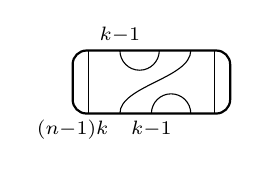
\begin{tikzpicture}[baseline = .3cm]
	\draw[thick, rounded corners = 5pt] (0,0) rectangle (2,.8);
	\draw (.2,0) -- (.2,.8);
	\draw (1.8,0) -- (1.8,.8);
	\draw (.6,.8) arc (-180:0:.25cm);
%	\draw (1.5,.8) arc (-180:0:.15cm);
	\draw (.6,0)  .. controls ++(90:.35cm) and ++(270:.35cm) .. (1.5,.8);
	\draw (1,0) arc (180:0:.25cm);
%	\node at (.7,-.2) {\scriptsize{$1$}};
%	\node at (1.8,1) {\scriptsize{$1$}};
%	\node at (2,-.2) {\scriptsize{$1$}};
	\node at (.6,1) {\scriptsize{$k{-}1$}};
	\node at (1,-.2) {\scriptsize{$k{-}1$}};
	\node at (0,-.2) {\scriptsize{$(n{-}1)k$}};
\end{tikzpicture}
\\&=
M_{(n+1)k-1} 
e_{(n+1)k-1}
\cdot \,
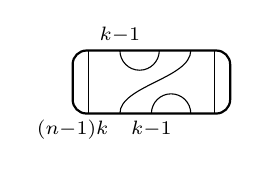
\begin{tikzpicture}[baseline = .3cm]
	\draw[thick, rounded corners = 5pt] (0,0) rectangle (2,.8);
	\draw (.2,0) -- (.2,.8);
	\draw (1.8,0) -- (1.8,.8);
	\draw (.6,.8) arc (-180:0:.25cm);
%	\draw (1.5,.8) arc (-180:0:.15cm);
	\draw (.6,0)  .. controls ++(90:.35cm) and ++(270:.35cm) .. (1.5,.8);
	\draw (1,0) arc (180:0:.25cm);
%	\node at (.7,-.2) {\scriptsize{$1$}};
%	\node at (1.8,1) {\scriptsize{$1$}};
%	\node at (2,-.2) {\scriptsize{$1$}};
	\node at (.6,1) {\scriptsize{$k{-}1$}};
	\node at (1,-.2) {\scriptsize{$k{-}1$}};
	\node at (0,-.2) {\scriptsize{$(n{-}1)k$}};
\end{tikzpicture}
=
M_{(n+1)k-1} 
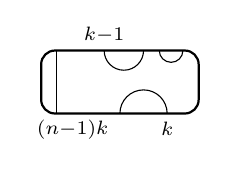
\begin{tikzpicture}[baseline = .3cm]
	\draw[thick, rounded corners = 5pt] (0,0) rectangle (2,.8);
	\draw (.2,0) -- (.2,.8);
	\draw (.8,.8) arc (-180:0:.25cm);
	\draw (1.5,.8) arc (-180:0:.15cm);
	\draw (1,0) arc (180:0:.3cm);
	\node at (.8,1) {\scriptsize{$k{-}1$}};
	\node at (1.6,-.2) {\scriptsize{$k$}};
	\node at (.4,-.2) {\scriptsize{$(n{-}1)k$}};
\end{tikzpicture}
\,.
\end{align*}
Since we may perform isotopy in the Temerley-Lieb-Jones subalgebra of $M_{(n+1)k}$, we may decompose the diagram on the right hand side as follows:
$$
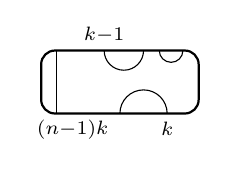
\begin{tikzpicture}[baseline = .3cm]
	\draw[thick, rounded corners = 5pt] (0,0) rectangle (2,.8);
	\draw (.2,0) -- (.2,.8);
	\draw (.8,.8) arc (-180:0:.25cm);
	\draw (1.5,.8) arc (-180:0:.15cm);
	\draw (1,0) arc (180:0:.3cm);
	\node at (.8,1) {\scriptsize{$k{-}1$}};
	\node at (1.6,-.2) {\scriptsize{$k$}};
	\node at (.4,-.2) {\scriptsize{$(n{-}1)k$}};
\end{tikzpicture}
=
d^{k-2}
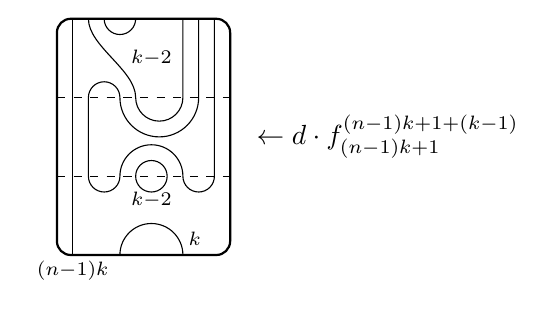
\begin{tikzpicture}[baseline = 1.4cm]
	\draw[thick, rounded corners = 5pt] (0,0) rectangle (2.2,3);
	\draw (.2,0) -- (.2,3);
	\draw (.6,3) arc (-180:0:.2cm);
	\draw (.4,3) .. controls ++(270:.35cm) and ++(90:.35cm) .. (1,2) arc (-180:0:.3cm) -- (1.6,3);
	\draw (1.8,3) -- (1.8,2) arc (0:-180:.5cm) arc (0:180:.2cm) -- (.4,1) arc (-180:0:.2cm) arc (180:0:.4cm) arc (-180:0:.2cm) -- (2,3);
	\draw (1.2,1) circle (.2cm);
	\draw (.8,0) arc (180:0:.4cm);
	\draw[dashed] (0,1) -- (2.2,1);
	\draw[dashed] (0,2) -- (2.2,2);
	\node at (1.2,.7) {\scriptsize{$k{-}2$}};
	\node at (1.2,2.5) {\scriptsize{$k{-}2$}};
	\node at (1.75,.2) {\scriptsize{$k$}};
	\node at (.2,-.2) {\scriptsize{$(n{-}1)k$}};
%
	\node at (4.2,1.5) {$\leftarrow d\cdot f^{(n-1)k+1+(k-1)}_{(n-1)k+1}$};
\end{tikzpicture}
$$
By the induction hypothesis, we have
%\dave{used induction hypothesis for arbitrary $j$, which I set to zero earlier. 
%This isn't the biggest deal, but it's not technically correct.}
$$
M_{(n+1)k-1}
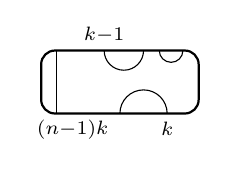
\begin{tikzpicture}[baseline = .3cm]
	\draw[thick, rounded corners = 5pt] (0,0) rectangle (2,.8);
	\draw (.2,0) -- (.2,.8);
	\draw (.8,.8) arc (-180:0:.25cm);
	\draw (1.5,.8) arc (-180:0:.15cm);
	\draw (1,0) arc (180:0:.3cm);
	\node at (.8,1) {\scriptsize{$k{-}1$}};
	\node at (1.6,-.2) {\scriptsize{$k$}};
	\node at (.4,-.2) {\scriptsize{$(n{-}1)k$}};
\end{tikzpicture}
=
M_{nk+(k-1)}
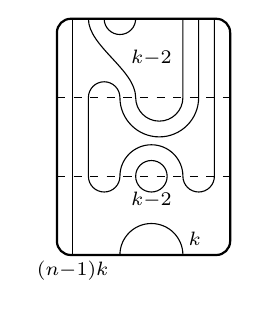
\begin{tikzpicture}[baseline = 1.4cm]
	\draw[thick, rounded corners = 5pt] (0,0) rectangle (2.2,3);
	\draw (.2,0) -- (.2,3);
	\draw (.6,3) arc (-180:0:.2cm);
	\draw (.4,3) .. controls ++(270:.35cm) and ++(90:.35cm) .. (1,2) arc (-180:0:.3cm) -- (1.6,3);
	\draw (1.8,3) -- (1.8,2) arc (0:-180:.5cm) arc (0:180:.2cm) -- (.4,1) arc (-180:0:.2cm) arc (180:0:.4cm) arc (-180:0:.2cm) -- (2,3);
	\draw (1.2,1) circle (.2cm);
	\draw (.8,0) arc (180:0:.4cm);
	\draw[dashed] (0,1) -- (2.2,1);
	\draw[dashed] (0,2) -- (2.2,2);
	\node at (1.2,.7) {\scriptsize{$k{-}2$}};
	\node at (1.2,2.5) {\scriptsize{$k{-}2$}};
	\node at (1.75,.2) {\scriptsize{$k$}};
	\node at (.2,-.2) {\scriptsize{$(n{-}1)k$}};
\end{tikzpicture}
=
M_{nk}\,
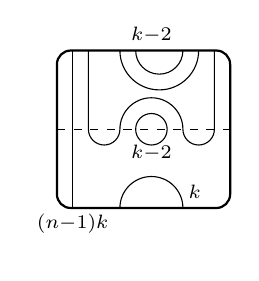
\begin{tikzpicture}[baseline = .9cm]
	\draw[thick, rounded corners = 5pt] (0,0) rectangle (2.2,2);
	\draw (.2,0) -- (.2,2);
	\draw (1,2) arc (-180:0:.3cm);
	\draw (1.8,2) arc (0:-180:.5cm); 
	\draw (.4,2) -- (.4,1) arc (-180:0:.2cm) arc (180:0:.4cm) arc (-180:0:.2cm) -- (2,2);
	\draw (1.2,1) circle (.2cm);
	\draw (.8,0) arc (180:0:.4cm);
	\draw[dashed] (0,1) -- (2.2,1);
	\node at (1.2,.7) {\scriptsize{$k{-}2$}};
	\node at (1.2,2.2) {\scriptsize{$k{-}2$}};
	\node at (1.75,.2) {\scriptsize{$k$}};
	\node at (.2,-.2) {\scriptsize{$(n{-}1)k$}};
\end{tikzpicture}
=
M_{nk} g_n.
$$
This completes the proof.
\end{proof}



%%%%%%%%%%%%%%%%%%%%%%%%%%%%%%%%%%%%%%%%%%%%%%%%%%%%%%%
\subsection{The projection category of a Markov tower}

We now define the category of projections of a Markov tower. 


\begin{defn}
\label{def:MarkovProjections}
Let $M_\bullet = (M_n, \tr_n, e_{n+1})$ be a Markov tower.
We define the category $\cM$ to be the unitary Karoubi completion (formally adding orthogonal direct sums, and then taking the orthogonal projection completion) of the $\Cstar$ category $\cM_0$ with finite dimensional hom spaces defined as follows.
\begin{itemize}
\item
The objects of $\cM_0$ are the symbols $[n]$ for $n\geq 0$.
\item
Given $n,k \geq 0$, we define 
$\cM_0([n] \to [n+2k]):= M_{n+k}$
and
$\cM_0([n+2k] \to [n]) := M_{n+k}$.
\item
The identity morphism in $\cM_0([n] \to [n])$ is $1_{M_n}$.
\item
For $x\in \cM_0([n]\to [n+2k])$ or $x\in \cM_0([n+2k] \to [n])$, we define $x^\dag := x^* \in M_{n+k}$.
%
%\begin{align*}
%\cM([n] \to n+2k])
%&:=
%%\set{x \in M_{n+k}}{ x = E^{M_{n+2k}}_{M_{n+k}}(q x f^{n+k}_{n}p)}
%%=
%M_{n+k}.
%q
%M_{n+k}
%f^{n+k}_n
%p
%\subset
%M_{n+2k}
%\\
%\cM(q \to p)
%&:=
%%\set{x \in M_{n+k}}{ x = E^{M_{n+2k}}_{M_{n+k}}(q x f^{n+k}_{n}p)}
%%=
%p
%f^{n+k}_n
%M_{n+k}
%q
%\subset
%M_{n+2k}
%\end{align*}
%where $f^{n+k}_{n}\in M_{n+2k} = M_{n+k} f^{n+k}_n M_{n+k}$ is the Jones projection for the \nn{standard} inclusion $M_n \subset M_k \subset (M_{n+2k}, \tr_{n+2k}, f^{n+k}_n)$.
%We define $\cM(q \to p) := \cM(p \to q)^\dag =  \set{x^\dag}{x\in \cM(p \to q)}$.
\item
We define composition in three cases.
\begin{enumerate}[label={\rm(C\arabic*)}]
\item
\label{compose:upup}
If $x\in \cM_0([n] \to [n+2j])$ and $y\in \cM_0([n+2j] \to [n+2j+2k])$, we define 
$$
y\circ x
:=
E^{n+2j+k}_{n+j+k}
\left(
\raisebox{.3cm}{$
\underbrace{
y\cdot x \cdot
d^{-j}\,
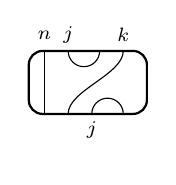
\begin{tikzpicture}[baseline = .3cm]
	\draw[thick, rounded corners = 5pt] (0,0) rectangle (1.5,.8);
	\draw (.2,0) -- (.2,.8);
	\draw (.5,.8) arc (-180:0:.2cm);
	\draw (.5,0) .. controls ++(90:.3cm) and ++(270:.3cm) .. (1.2,.8);
	\draw (.8,0) arc (180:0:.2cm);
	\node at (.2,1) {\scriptsize{$n$}};
	\node at (.5,1) {\scriptsize{$j$}};
	\node at (1.2,1) {\scriptsize{$k$}};
	\node at (.8,-.2) {\scriptsize{$j$}};
\end{tikzpicture}
}_{\in M_{n+2j+k}}
$}
\right)
\in M_{n+j+k}
=
\cM_0([n] \to [n+2j+2k]).
$$
We define the composite $x^\dag \circ y^\dag := (y\circ x)^\dag$, which defines composition 
$\cM_0([n+2j+2k] \to [n+2j]) \otimes \cM_0([n+2j] \to [n]) \to \cM_0([n+2j+2k] \to [n])$.
To show $x^\dag \circ y^\dag$ is well-defined, we check that when $j=k=0$,
\begin{equation}
\label{eq:n to n to n}
x^\dag\circ y^\dag= x^* y^* = (y x)^* = (y\circ x)^\dag.
\end{equation}

\item
\label{compose:updown}
If $x\in \cM_0([n] \to [n+2j])$ and $y \in \cM_0([m+2k] \to [m])$
with $n+2j = m+2k$, $m= n + 2\ell$, and $j = k+\ell$,
we define
$$
y\circ x
:=
E^{n+2\ell + k}_{n+\ell}
\left(
\raisebox{.3cm}{$
\underbrace{
y\cdot x\cdot
d^{-\ell}\,
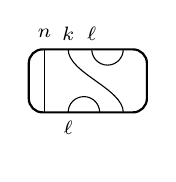
\begin{tikzpicture}[baseline = .3cm]
	\draw[thick, rounded corners = 5pt] (0,0) rectangle (1.5,.8);
	\draw (.2,0) -- (.2,.8);
	\draw (.8,.8) arc (-180:0:.2cm);
	\draw (1.2,0) .. controls ++(90:.3cm) and ++(270:.3cm) .. (.5,.8);
	\draw (.5,0) arc (180:0:.2cm);
	\node at (.2,1) {\scriptsize{$n$}};
	\node at (.5,1) {\scriptsize{$k$}};
	\node at (.8,1) {\scriptsize{$\ell$}};
	\node at (.5,-.2) {\scriptsize{$\ell$}};
\end{tikzpicture}
}_{\in M_{n+2\ell +k}}
$}
\right)
\in
M_{n+\ell}
=
\cM_0([n] \to [m]).
$$
As above, we define the composite $x^\dag \circ y^\dag := (y\circ x)^\dag$, which defines composition
$\cM_0([m] \to [m+2k]) \otimes \cM_0([n+2j] \to [n]) \to \cM_0([m] \to [n])$.
To show that $x^\dag \circ y^\dag$ is well-defined, we check that when $\ell=0$ so that $n=m$, 
\begin{equation}
\label{eq:n to n+2k to n}
x^\dag \circ y^\dag 
=
E^{n+k}_{n}(x^* y^*)
=
E^{n+k}_{n}((yx)^*) 
=
E^{n+k}_{n}(y x)^*
=
(y\circ x)^\dag.
\end{equation}

\item
\label{compose:downup}
If $x\in \cM_0([n+2j] \to [n])$ and $y\in \cM_0([n] \to [n+2k])$ with $k=j+\ell$, we define
$$
y\circ x 
:=
y\cdot
d^{-j}\,
\begin{tikzpicture}[baseline = .3cm]
	\draw[thick, rounded corners = 5pt] (0,0) rectangle (1.5,.8);
	\draw (.2,0) -- (.2,.8);
	\draw (.8,.8) arc (-180:0:.2cm);
	\draw (1.2,0) .. controls ++(90:.3cm) and ++(270:.3cm) .. (.5,.8);
	\draw (.5,0) arc (180:0:.2cm);
	\node at (.2,1) {\scriptsize{$n$}};
	\node at (.5,1) {\scriptsize{$\ell$}};
	\node at (.8,1) {\scriptsize{$j$}};
	\node at (.5,-.2) {\scriptsize{$j$}};
\end{tikzpicture}
\cdot x
\in
M_{n+2j+\ell}
=
\cM_0([n+2j] \to [n+2k]).
$$
As above, we define the composite $x^\dag \circ y^\dag := (y\circ x)^\dag$, which defines composition
$\cM_0([n+2k] \to [n]) \otimes \cM_0([n] \to [n+2j]) \to \cM_0([n+2k] \to [n+2j])$.
To show that $x^\dag \circ y^\dag$ is well-defined, we check that when $\ell=0$ so that $j=k$, 
\begin{equation}
\label{eq:n+2j to n to n+2j}
x^\dag \circ y^\dag 
=
x^* \cdot
d^{-j}\,
\begin{tikzpicture}[baseline = .3cm]
	\draw[thick, rounded corners = 5pt] (0,0) rectangle (1.2,.8);
	\draw (.2,0) -- (.2,.8);
	\draw (.5,.8) arc (-180:0:.2cm);
	\draw (.5,0) arc (180:0:.2cm);
	\node at (.2,1) {\scriptsize{$n$}};
	\node at (.5,1) {\scriptsize{$j$}};
	\node at (.5,-.2) {\scriptsize{$j$}};
\end{tikzpicture}
\cdot y^*
=
\left(
y \cdot
d^{-j}\,
\begin{tikzpicture}[baseline = .3cm]
	\draw[thick, rounded corners = 5pt] (0,0) rectangle (1.2,.8);
	\draw (.2,0) -- (.2,.8);
	\draw (.5,.8) arc (-180:0:.2cm);
	\draw (.5,0) arc (180:0:.2cm);
	\node at (.2,1) {\scriptsize{$n$}};
	\node at (.5,1) {\scriptsize{$j$}};
	\node at (.5,-.2) {\scriptsize{$j$}};
\end{tikzpicture}
\cdot x
\right)^*
=
(y\circ x)^\dag.
\end{equation}
\end{enumerate}
\end{itemize}
Showing that composition is associative directly from the definitions above is a highly non-trivial exercise using the axioms \ref{eq:MarkovJonesProjections} -- \ref{eq:MarkovPullDown} of a Markov tower.
A better way to prove associativity is to prove that each $4\times 4$ (possibly non-associative) \emph{linking algebra} \cite{MR808930} 
$\cL:=(\cM_0([a] \to[b]))_{a,b}$ where $a,b\in \{n, n+2j, n+2j+2k, n+2j+2k+2\ell\}$
is $\dag/*$-isomorphic to a von Neumann algebra, which is necessarily associative!
This technique also offers the advantage that it, simultaneously proves $\cM_0$ is $\Cstar$.\footnote{
Just as being a $\Cstar$ algebra is a property of a complex $*$-algebra, being a $\Cstar$ category is a property of a $\bbC$-linear dagger category.
}

Notice we have an equality of sets
\begin{equation}
\label{eq:LinkingAlgebra}
\cL=
\left(
\begin{array}{llll}
M_n & M_{n{+}j} & M_{n{+}j{+}k} & M_{n{+}j{+}k{+}\ell}
\\
M_{n{+}j} & M_{n{+}2j} & M_{n{+}2j{+}k} & M_{n{+}2j{+}k{+}\ell}
\\
M_{n{+}j{+}k} & M_{n{+}2j{+}k} & M_{n{+}2j{+}2k} & M_{n{+}2j{+}2k{+}\ell}
\\
M_{n{+}j{+}k{+}\ell} & M_{n{+}2j{+}k{+}\ell} & M_{n{+}2j{+}2k{+}\ell} & M_{n{+}2j{+}2k{+}2\ell}
\end{array}
\right).
\end{equation}
We define the following map entry-wise; that is, for an element $x \in \cL$, we plug $x_{ab}$ into the input disk in the $ab$-th entry of the map $\pi :\cL \to pM_4(M_{n+2j+2k+2\ell})p$
\begin{equation}
\label{eq:4x4Map}
\resizebox{.92\hsize}{!}{
$
\begin{pmatrix}
d^{{-}j{-}k{-}\ell}\,
\begin{tikzpicture}[baseline=-.1cm]
	\draw (.2,.6) arc (-180:0:.2cm);
	\draw (.2,-.6) arc (180:0:.2cm);
	\draw (.8,.6) arc (-180:0:.2cm);
	\draw (.8,-.6) arc (180:0:.2cm);
	\draw (1.4,.6) arc (-180:0:.2cm);
	\draw (1.4,-.6) arc (180:0:.2cm);
	\draw (0,-.6) -- (0,.6);
	\roundNbox{unshaded}{(0,0)}{.2}{0}{0}{}
	\node at (0,-.8) {\scriptsize{$n$}};
	\node at (0,.8) {\scriptsize{$n$}};
	\node at (.2,.8) {\scriptsize{$j$}};
	\node at (.6,.8) {\scriptsize{$j$}};
	\node at (.8,.8) {\scriptsize{$k$}};
	\node at (1.2,.8) {\scriptsize{$k$}};
	\node at (1.4,.8) {\scriptsize{$\ell$}};
	\node at (1.8,.8) {\scriptsize{$\ell$}};
	\node at (.2,-.8) {\scriptsize{$j$}};
	\node at (.6,-.8) {\scriptsize{$j$}};
	\node at (.8,-.8) {\scriptsize{$k$}};
	\node at (1.2,-.8) {\scriptsize{$k$}};
	\node at (1.4,-.8) {\scriptsize{$\ell$}};
	\node at (1.8,-.8) {\scriptsize{$\ell$}};
\end{tikzpicture}
& 
d^{{-}j{-}k{-}\ell}\,
\begin{tikzpicture}[baseline=-.1cm]
	\draw (.2,.6) arc (-180:0:.2cm);
	\draw (.2,-.6) -- (.2,.1) arc (180:0:.2cm) -- (.6,-.6);
	\draw (.8,.6) arc (-180:0:.2cm);
	\draw (.8,-.6) arc (180:0:.2cm);
	\draw (1.4,.6) arc (-180:0:.2cm);
	\draw (1.4,-.6) arc (180:0:.2cm);
	\draw (0,-.6) -- (0,.6);
	\roundNbox{unshaded}{(0,-.1)}{.2}{0}{.2}{}
	\node at (0,-.8) {\scriptsize{$n$}};
	\node at (0,.8) {\scriptsize{$n$}};
	\node at (.2,.8) {\scriptsize{$j$}};
	\node at (.6,.8) {\scriptsize{$j$}};
	\node at (.8,.8) {\scriptsize{$k$}};
	\node at (1.2,.8) {\scriptsize{$k$}};
	\node at (1.4,.8) {\scriptsize{$\ell$}};
	\node at (1.8,.8) {\scriptsize{$\ell$}};
	\node at (.2,-.8) {\scriptsize{$j$}};
	\node at (.6,-.8) {\scriptsize{$j$}};
	\node at (.8,-.8) {\scriptsize{$k$}};
	\node at (1.2,-.8) {\scriptsize{$k$}};
	\node at (1.4,-.8) {\scriptsize{$\ell$}};
	\node at (1.8,-.8) {\scriptsize{$\ell$}};
\end{tikzpicture}
&
d^{{-}j{-}k{-}\ell}\,
\begin{tikzpicture}[baseline=-.1cm]
	\draw (.2,-.6) -- (.2,0) .. controls ++(90:.45cm) and ++(90:.45cm) .. (1.2,0) -- (1.2,-.6);
	\draw (.4,-.6) -- (.4,0) .. controls ++(90:.2cm) and ++(90:.2cm) ..  (1,0) -- (1,-.6);
	\draw (.2,.6) arc (-180:0:.2cm);
	\draw (.8,.6) arc (-180:0:.2cm);
	\draw (1.4,.6) arc (-180:0:.2cm);
	\draw (1.4,-.6) arc (180:0:.2cm);
	\draw (0,-.6) -- (0,.6);
	\roundNbox{unshaded}{(0,-.2)}{.2}{0}{.4}{}
	\node at (0,-.8) {\scriptsize{$n$}};
	\node at (0,.8) {\scriptsize{$n$}};
	\node at (.2,.8) {\scriptsize{$j$}};
	\node at (.6,.8) {\scriptsize{$j$}};
	\node at (.8,.8) {\scriptsize{$k$}};
	\node at (1.2,.8) {\scriptsize{$k$}};
	\node at (1.4,.8) {\scriptsize{$\ell$}};
	\node at (1.8,.8) {\scriptsize{$\ell$}};
	\node at (.2,-.8) {\scriptsize{$j$}};
	\node at (.4,-.8) {\scriptsize{$k$}};
	\node at (1,-.8) {\scriptsize{$k$}};
	\node at (1.2,-.8) {\scriptsize{$j$}};
	\node at (1.4,-.8) {\scriptsize{$\ell$}};
	\node at (1.8,-.8) {\scriptsize{$\ell$}};
\end{tikzpicture}
&
d^{{-}j{-}k{-}\ell}\,
\begin{tikzpicture}[baseline=-.1cm]
	\draw (.2,-.6) -- (.2,0) .. controls ++(90:.45cm) and ++(90:.45cm) .. (1.8,0) -- (1.8,-.6);
	\draw (.4,-.6) -- (.4,0) .. controls ++(90:.3cm) and ++(90:.3cm) ..  (1.4,0) -- (1.4,-.6);
	\draw (.6,-.6) -- (.6,0) .. controls ++(90:.15cm) and ++(90:.15cm) ..  (1,0) -- (1,-.6);
	\draw (.2,.6) arc (-180:0:.2cm);
	\draw (.8,.6) arc (-180:0:.2cm);
	\draw (1.4,.6) arc (-180:0:.2cm);
	\draw (0,-.6) -- (0,.6);
	\roundNbox{unshaded}{(0,-.2)}{.2}{0}{.6}{}
	\node at (0,-.8) {\scriptsize{$n$}};
	\node at (0,.8) {\scriptsize{$n$}};
	\node at (.2,.8) {\scriptsize{$j$}};
	\node at (.6,.8) {\scriptsize{$j$}};
	\node at (.8,.8) {\scriptsize{$k$}};
	\node at (1.2,.8) {\scriptsize{$k$}};
	\node at (1.4,.8) {\scriptsize{$\ell$}};
	\node at (1.8,.8) {\scriptsize{$\ell$}};
	\node at (.2,-.8) {\scriptsize{$j$}};
	\node at (.4,-.8) {\scriptsize{$k$}};
	\node at (.6,-.8) {\scriptsize{$\ell$}};
	\node at (1,-.8) {\scriptsize{$\ell$}};
	\node at (1.4,-.8) {\scriptsize{$k$}};
	\node at (1.8,-.8) {\scriptsize{$j$}};
\end{tikzpicture}
\\
d^{{-}j{-}k{-}\ell}\,
\begin{tikzpicture}[baseline=-.1cm, yscale = -1]
	\draw (.2,.6) arc (-180:0:.2cm);
	\draw (.8,.6) arc (-180:0:.2cm);
	\draw (.2,-.6) -- (.2,.1) arc (180:0:.2cm) -- (.6,-.6);
	\draw (.8,-.6) arc (180:0:.2cm);
	\draw (1.4,.6) arc (-180:0:.2cm);
	\draw (1.4,-.6) arc (180:0:.2cm);
	\draw (0,-.6) -- (0,.6);
	\roundNbox{unshaded}{(0,-.1)}{.2}{0}{.2}{}
	\node at (0,-.8) {\scriptsize{$n$}};
	\node at (0,.8) {\scriptsize{$n$}};
	\node at (.2,.8) {\scriptsize{$j$}};
	\node at (.6,.8) {\scriptsize{$j$}};
	\node at (.8,.8) {\scriptsize{$k$}};
	\node at (1.2,.8) {\scriptsize{$k$}};
	\node at (1.4,.8) {\scriptsize{$\ell$}};
	\node at (1.8,.8) {\scriptsize{$\ell$}};
	\node at (.2,-.8) {\scriptsize{$j$}};
	\node at (.6,-.8) {\scriptsize{$j$}};
	\node at (.8,-.8) {\scriptsize{$k$}};
	\node at (1.2,-.8) {\scriptsize{$k$}};
	\node at (1.4,-.8) {\scriptsize{$\ell$}};
	\node at (1.8,-.8) {\scriptsize{$\ell$}};
\end{tikzpicture}
&
d^{{-}k{-}\ell}\,
\begin{tikzpicture}[baseline=-.1cm]
	\draw (.6,.6) arc (-180:0:.2cm);
	\draw (.6,-.6) arc (180:0:.2cm);
	\draw (1.4,.6) arc (-180:0:.2cm);
	\draw (1.4,-.6) arc (180:0:.2cm);
	\draw (0,-.6) -- (0,.6);
	\roundNbox{unshaded}{(0,0)}{.2}{0}{0}{}
	\node at (0,-.8) {\scriptsize{$n{+}2j$}};
	\node at (0,.8) {\scriptsize{$n{+}2j$}};
	\node at (.6,.8) {\scriptsize{$k$}};
	\node at (1,.8) {\scriptsize{$k$}};
	\node at (1.4,.8) {\scriptsize{$\ell$}};
	\node at (1.8,.8) {\scriptsize{$\ell$}};
	\node at (.6,-.8) {\scriptsize{$k$}};
	\node at (1,-.8) {\scriptsize{$k$}};
	\node at (1.4,-.8) {\scriptsize{$\ell$}};
	\node at (1.8,-.8) {\scriptsize{$\ell$}};
\end{tikzpicture}
&
d^{{-}k{-}\ell}\,
\begin{tikzpicture}[baseline=-.1cm]
	\draw (.6,.6) arc (-180:0:.2cm);
	\draw (.6,-.6) -- (.6,.1) arc (180:0:.2cm) -- (1,-.6);
	\draw (1.4,.6) arc (-180:0:.2cm);
	\draw (1.4,-.6) arc (180:0:.2cm);
	\draw (0,-.6) -- (0,.6);
	\roundNbox{unshaded}{(0,-.1)}{.2}{0}{.6}{}
	\node at (0,-.8) {\scriptsize{$n{+}2j$}};
	\node at (0,.8) {\scriptsize{$n{+}2j$}};
	\node at (.6,.8) {\scriptsize{$k$}};
	\node at (.6,-.8) {\scriptsize{$k$}};
	\node at (1.4,.8) {\scriptsize{$\ell$}};
	\node at (1.8,.8) {\scriptsize{$\ell$}};
	\node at (1,.8) {\scriptsize{$k$}};
	\node at (1,-.8) {\scriptsize{$k$}};
	\node at (1.4,-.8) {\scriptsize{$\ell$}};
	\node at (1.8,-.8) {\scriptsize{$\ell$}};
\end{tikzpicture}
&
d^{{-}k{-}\ell}\,
\begin{tikzpicture}[baseline=-.1cm]
	\draw (.6,-.6) -- (.6,0) .. controls ++(90:.45cm) and ++(90:.45cm) ..  (1.6,0) -- (1.6,-.6);
	\draw (.8,-.6) -- (.8,0) .. controls ++(90:.3cm) and ++(90:.3cm) ..  (1.2,0) -- (1.2,-.6);
	\draw (.6,.6) arc (-180:0:.2cm);
	\draw (1.2,.6) arc (-180:0:.2cm);
	\draw (0,-.6) -- (0,.6);
	\roundNbox{unshaded}{(0,-.2)}{.2}{0}{.8}{}
	\node at (0,-.8) {\scriptsize{$n{+}2j$}};
	\node at (0,.8) {\scriptsize{$n{+}2j$}};
	\node at (.6,.8) {\scriptsize{$k$}};
	\node at (1,.8) {\scriptsize{$k$}};
	\node at (1.2,.8) {\scriptsize{$\ell$}};
	\node at (1.6,.8) {\scriptsize{$\ell$}};
	\node at (.6,-.8) {\scriptsize{$k$}};
	\node at (.8,-.8) {\scriptsize{$\ell$}};
	\node at (1.2,-.8) {\scriptsize{$\ell$}};
	\node at (1.6,-.8) {\scriptsize{$k$}};
\end{tikzpicture}
\\
d^{{-}j{-}k{-}\ell}\,
\begin{tikzpicture}[baseline=-.1cm, yscale = -1]
	\draw (.2,-.6) -- (.2,0) .. controls ++(90:.45cm) and ++(90:.45cm) .. (1.2,0) -- (1.2,-.6);
	\draw (.4,-.6) -- (.4,0) .. controls ++(90:.2cm) and ++(90:.2cm) ..  (1,0) -- (1,-.6);
	\draw (.2,.6) arc (-180:0:.2cm);
	\draw (.8,.6) arc (-180:0:.2cm);
	\draw (1.4,.6) arc (-180:0:.2cm);
	\draw (1.4,-.6) arc (180:0:.2cm);
	\draw (0,-.6) -- (0,.6);
	\roundNbox{unshaded}{(0,-.2)}{.2}{0}{.4}{}
	\node at (0,-.8) {\scriptsize{$n$}};
	\node at (0,.8) {\scriptsize{$n$}};
	\node at (.2,.8) {\scriptsize{$j$}};
	\node at (.6,.8) {\scriptsize{$j$}};
	\node at (.8,.8) {\scriptsize{$k$}};
	\node at (1.2,.8) {\scriptsize{$k$}};
	\node at (1.4,.8) {\scriptsize{$\ell$}};
	\node at (1.8,.8) {\scriptsize{$\ell$}};
	\node at (.2,-.8) {\scriptsize{$j$}};
	\node at (.4,-.8) {\scriptsize{$k$}};
	\node at (1,-.8) {\scriptsize{$k$}};
	\node at (1.2,-.8) {\scriptsize{$j$}};
	\node at (1.4,-.8) {\scriptsize{$\ell$}};
	\node at (1.8,-.8) {\scriptsize{$\ell$}};
\end{tikzpicture}
&
d^{-k-\ell}
\,
\begin{tikzpicture}[baseline=-.1cm, yscale =-1]
	\draw (.6,.6) arc (-180:0:.2cm);
	\draw (.6,-.6) -- (.6,.1) arc (180:0:.2cm) -- (1,-.6);
	\draw (1.4,.6) arc (-180:0:.2cm);
	\draw (1.4,-.6) arc (180:0:.2cm);
	\draw (0,-.6) -- (0,.6);
	\roundNbox{unshaded}{(0,-.1)}{.2}{0}{.6}{}
	\node at (0,-.8) {\scriptsize{$n{+}2j$}};
	\node at (0,.8) {\scriptsize{$n{+}2j$}};
	\node at (.6,.8) {\scriptsize{$k$}};
	\node at (.6,-.8) {\scriptsize{$k$}};
	\node at (1.4,.8) {\scriptsize{$\ell$}};
	\node at (1.8,.8) {\scriptsize{$\ell$}};
	\node at (1,.8) {\scriptsize{$k$}};
	\node at (1,-.8) {\scriptsize{$k$}};
	\node at (1.4,-.8) {\scriptsize{$\ell$}};
	\node at (1.8,-.8) {\scriptsize{$\ell$}};
\end{tikzpicture}
&
d^{-\ell}
\begin{tikzpicture}[baseline=-.1cm]
	\draw (0,-.6) -- (0,.6);
	\draw (.8,.6) arc (-180:0:.2cm);
	\draw (.8,-.6) arc (180:0:.2cm);
	\roundNbox{unshaded}{(0,0)}{.2}{0}{0}{}
	\node at (0,-.8) {\scriptsize{$n{+}2j{+}2k$}};
	\node at (0,.8) {\scriptsize{$n{+}2j{+}2k$}};
	\node at (.8,.8) {\scriptsize{$\ell$}};
	\node at (1.2,.8) {\scriptsize{$\ell$}};
	\node at (.8,-.8) {\scriptsize{$\ell$}};
	\node at (1.2,-.8) {\scriptsize{$\ell$}};
\end{tikzpicture}
&
d^{-\ell}\,
\begin{tikzpicture}[baseline=-.1cm]
	\draw (0,-.6) -- (0,.6);
	\draw (1,.6) arc (-180:0:.2cm);
	\draw (1,-.6) -- (1,.1) arc (180:0:.2cm) -- (1.4,-.6);
	\roundNbox{unshaded}{(0,-.1)}{.2}{0}{1}{}
	\node at (0,-.8) {\scriptsize{$n{+}2j{+}2k$}};
	\node at (0,.8) {\scriptsize{$n{+}2j{+}2k$}};
	\node at (1,.8) {\scriptsize{$\ell$}};
	\node at (1.4,.8) {\scriptsize{$\ell$}};
	\node at (1,-.8) {\scriptsize{$\ell$}};
	\node at (1.4,-.8) {\scriptsize{$\ell$}};
\end{tikzpicture}
\\
d^{{-}j{-}k{-}\ell}\,
\begin{tikzpicture}[baseline=-.1cm, yscale = -1]
	\draw (.2,-.6) -- (.2,0) .. controls ++(90:.45cm) and ++(90:.45cm) .. (1.8,0) -- (1.8,-.6);
	\draw (.4,-.6) -- (.4,0) .. controls ++(90:.3cm) and ++(90:.3cm) ..  (1.4,0) -- (1.4,-.6);
	\draw (.6,-.6) -- (.6,0) .. controls ++(90:.15cm) and ++(90:.15cm) ..  (1,0) -- (1,-.6);
	\draw (.2,.6) arc (-180:0:.2cm);
	\draw (.8,.6) arc (-180:0:.2cm);
	\draw (1.4,.6) arc (-180:0:.2cm);
	\draw (0,-.6) -- (0,.6);
	\roundNbox{unshaded}{(0,-.2)}{.2}{0}{.6}{}
	\node at (0,-.8) {\scriptsize{$n$}};
	\node at (0,.8) {\scriptsize{$n$}};
	\node at (.2,.8) {\scriptsize{$j$}};
	\node at (.6,.8) {\scriptsize{$j$}};
	\node at (.8,.8) {\scriptsize{$k$}};
	\node at (1.2,.8) {\scriptsize{$k$}};
	\node at (1.4,.8) {\scriptsize{$\ell$}};
	\node at (1.8,.8) {\scriptsize{$\ell$}};
	\node at (.2,-.8) {\scriptsize{$j$}};
	\node at (.4,-.8) {\scriptsize{$k$}};
	\node at (.6,-.8) {\scriptsize{$\ell$}};
	\node at (1,-.8) {\scriptsize{$\ell$}};
	\node at (1.4,-.8) {\scriptsize{$k$}};
	\node at (1.8,-.8) {\scriptsize{$j$}};
\end{tikzpicture}
&
d^{-k-\ell}
\begin{tikzpicture}[baseline=-.1cm, yscale = -1]
	\draw (.6,-.6) -- (.6,0) .. controls ++(90:.45cm) and ++(90:.45cm) ..  (1.6,0) -- (1.6,-.6);
	\draw (.8,-.6) -- (.8,0) .. controls ++(90:.3cm) and ++(90:.3cm) ..  (1.2,0) -- (1.2,-.6);
	\draw (.6,.6) arc (-180:0:.2cm);
	\draw (1.2,.6) arc (-180:0:.2cm);
	\draw (0,-.6) -- (0,.6);
	\roundNbox{unshaded}{(0,-.2)}{.2}{0}{.8}{}
	\node at (0,-.8) {\scriptsize{$n{+}2j$}};
	\node at (0,.8) {\scriptsize{$n{+}2j$}};
	\node at (.6,.8) {\scriptsize{$k$}};
	\node at (1,.8) {\scriptsize{$k$}};
	\node at (1.2,.8) {\scriptsize{$\ell$}};
	\node at (1.6,.8) {\scriptsize{$\ell$}};
	\node at (.6,-.8) {\scriptsize{$k$}};
	\node at (.8,-.8) {\scriptsize{$\ell$}};
	\node at (1.2,-.8) {\scriptsize{$\ell$}};
	\node at (1.6,-.8) {\scriptsize{$k$}};
\end{tikzpicture}
&
d^{-\ell}
\begin{tikzpicture}[baseline=-.1cm, yscale = -1]
	\draw (0,-.6) -- (0,.6);
	\draw (1,.6) arc (-180:0:.2cm);
	\draw (1,-.6) -- (1,.1) arc (180:0:.2cm) -- (1.4,-.6);
	\roundNbox{unshaded}{(0,-.1)}{.2}{0}{1}{}
	\node at (0,-.8) {\scriptsize{$n{+}2j{+}2k$}};
	\node at (0,.8) {\scriptsize{$n{+}2j{+}2k$}};
	\node at (1,.8) {\scriptsize{$\ell$}};
	\node at (1.4,.8) {\scriptsize{$\ell$}};
	\node at (1,-.8) {\scriptsize{$\ell$}};
	\node at (1.4,-.8) {\scriptsize{$\ell$}};
\end{tikzpicture}
&
\begin{tikzpicture}[baseline=-.1cm, yscale =-1]
	\draw (0,-.6) -- (0,.6);
	\roundNbox{unshaded}{(0,0)}{.2}{0}{0}{}
	\node at (0,-.8) {\scriptsize{$n{+}2j{+}2k{+}2\ell$}};
	\node at (0,.8) {\scriptsize{$n{+}2j{+}2k{+}2\ell$}};
\end{tikzpicture}
\end{pmatrix}
$}
\end{equation}
where $p\in M_4(M_{n+2j+2k+2\ell})$ is the following projection:
$$
p:=
\operatorname{diag}\left(
d^{{-}j{-}k{-}\ell}\,
\begin{tikzpicture}[baseline = -.1cm]
	\draw[thick, rounded corners = 5pt] (-.2,-.3) rectangle (2,.3);
	\draw (.2,.3) arc (-180:0:.2cm);
	\draw (.2,-.3) arc (180:0:.2cm);
	\draw (.8,.3) arc (-180:0:.2cm);
	\draw (.8,-.3) arc (180:0:.2cm);
	\draw (1.4,.3) arc (-180:0:.2cm);
	\draw (1.4,-.3) arc (180:0:.2cm);
	\draw (0,-.3) -- (0,.3);
	\node at (0,-.5) {\scriptsize{$n$}};
	\node at (0,.5) {\scriptsize{$n$}};
	\node at (.2,.5) {\scriptsize{$j$}};
	\node at (.6,.5) {\scriptsize{$j$}};
	\node at (.8,.5) {\scriptsize{$k$}};
	\node at (1.2,.5) {\scriptsize{$k$}};
	\node at (1.4,.5) {\scriptsize{$\ell$}};
	\node at (1.8,.5) {\scriptsize{$\ell$}};
	\node at (.2,-.5) {\scriptsize{$j$}};
	\node at (.6,-.5) {\scriptsize{$j$}};
	\node at (.8,-.5) {\scriptsize{$k$}};
	\node at (1.2,-.5) {\scriptsize{$k$}};
	\node at (1.4,-.5) {\scriptsize{$\ell$}};
	\node at (1.8,-.5) {\scriptsize{$\ell$}};
\end{tikzpicture}
\,,
d^{-k-\ell}
\begin{tikzpicture}[baseline = -.1cm]
	\draw[thick, rounded corners = 5pt] (-.2,-.3) rectangle (1.8,.3);
	\draw (.6,.3) arc (-180:0:.2cm);
	\draw (.6,-.3) arc (180:0:.2cm);
	\draw (1.2,.3) arc (-180:0:.2cm);
	\draw (1.2,-.3) arc (180:0:.2cm);
	\draw (0,-.3) -- (0,.3);
	\node at (0,-.5) {\scriptsize{$n{+}2j$}};
	\node at (0,.5) {\scriptsize{$n{+}2j$}};
	\node at (.6,.5) {\scriptsize{$k$}};
	\node at (1,.5) {\scriptsize{$k$}};
	\node at (1.2,.5) {\scriptsize{$\ell$}};
	\node at (1.6,.5) {\scriptsize{$\ell$}};
	\node at (.6,-.5) {\scriptsize{$k$}};
	\node at (1,-.5) {\scriptsize{$k$}};
	\node at (1.2,-.5) {\scriptsize{$\ell$}};
	\node at (1.6,-.5) {\scriptsize{$\ell$}};
\end{tikzpicture}
\,,
d^{-\ell}
\begin{tikzpicture}[baseline = -.1cm]
	\draw[thick, rounded corners = 5pt] (-.2,-.3) rectangle (1.4,.3);
	\draw (.8,.3) arc (-180:0:.2cm);
	\draw (.8,-.3) arc (180:0:.2cm);
	\draw (0,-.3) -- (0,.3);
	\node at (0,-.5) {\scriptsize{$n{+}2j{+}2k$}};
	\node at (0,.5) {\scriptsize{$n{+}2j{+}2k$}};
	\node at (.8,.5) {\scriptsize{$\ell$}};
	\node at (1.2,.5) {\scriptsize{$\ell$}};
	\node at (.8,-.5) {\scriptsize{$\ell$}};
	\node at (1.2,-.5) {\scriptsize{$\ell$}};
\end{tikzpicture}
\,,
1_{n+2j+2k+2\ell}
\right).
$$
In Proposition \ref{prop:InjectiveAlgebraMap} below, we verify the map $\pi$ is an injective unital algebra map satisfying $\pi(x^\dag) = \pi(x)^*$, and is thus an isomorphism onto its image.
Thus $\im(\pi)$ is a unital $*$-subalgebra of the finite dimensional von Neumann algebra $pM_4(M_{n+2j+2k+2\ell})p$, which meanss $\im(\pi)$ is a von Neumann algebra by the finite dimensional bicommutant theorem \cite[Thm.~3.2.1]{JonesVNA}.
By looking at the $2\times 2$ and $3\times 3$ corners of the linking algebra $\cL$ and \eqref{eq:4x4Map},
we immediately see: 
\begin{itemize}
\item
$\dag$ is a dagger structure on $\cM_0$,
\item
for every $f\in \cM_0([n]\to [n+2k])$, there is a $g\in \cM_0([n] \to [n])$ and an $h\in \cM_0([n+2k]\to [n+2k])$ such that 
$f^\dag \circ f = g^\dag \circ g$ and $f\circ f^\dag = h^\dag \circ h$, and
\item
there are (pullback) norms on the (finite dimensional) hom spaces $\cM_0([n]\to [n+2j])$ and $\cM_0([n+2k] \to [n])$ which are sub-multiplicative with respect to composition and which satisfy the $\Cstar$ axiom $\|f^\dag \circ f \| = \|f^2\|$.\footnote{
Notice that in a $\Cstar$ category, these norm can be recovered from spectral radii together with the positivity and $\Cstar$ axioms.
Thus these norms are \emph{not} part of the data of the $\Cstar$ category.
}
\end{itemize}
Hence $\cM_0$ is $\Cstar$, and thus so is its unitary Karoubi completion $\cM$.
%In Proposition \ref{prop:MarkovAssociative} below, we verify that composition is associative.
%It follows immediately from the definition of composition that $\dag$ is a well-defined dagger structure on $\cM_0$.
%In Proposition \ref{prop:MarkovCstar} below, we verify $\cM_0$ is a $\Cstar$ category under this dagger structure.
\end{defn}


\begin{prop}
\label{prop:InjectiveAlgebraMap}
The map $\pi: \cL \to pM_4(M_{n+2j+2k+2\ell})p$ from Definition \ref{def:MarkovProjections} is an injective algebra map such that $\pi(x^\dag) = \pi(x)^*$ for all $x\in \cL$.
\end{prop}
\begin{proof}
	From equation \ref{eq:LinkingAlgebra}, it is clear that $\pi$ is injective, unital, and respects the $\dag$-structure. The difficulty is in seeing that $\pi$ is an algebra homomorphism. 
\nn{Use Proposition \ref{prop:MultistepJonesProjections}}
\end{proof}

\begin{cor}
\label{cor:SemisimpleProjectionCategory}
Let $M_\bullet$ be a Markov sequence and let $\cM$ be its unitarliy Karoubi complete $\Cstar$ category of projections.
Then $\cM$ is semisimple, and the isomorphism classes of simple objects are in canonical bijection with the vertices of the principal graph.
\end{cor}
\begin{proof}
All endomorphism algebras of $\cM$ are finite dimensional $\Cstar$ algebras which are semisimple, and thus $\cM$ is semisimple. By \ref{EP:BasicContruction}, every minimal projection in $X_{n+2}$ for $n\geq 0$ is equivalent to a minimal projection in $M_{n}$ via a parial isometry in $\cM_0([n] \to [n+2])$. 
Explicitly, $p\in M_n$ is equivalent to $p e_{n+1} \in M_{n+2}$ via the morphism $p\in M_{n+1} = \cM_0([n] \to [n+2])$, which is a partial isometry using the definition of composition \ref{compose:updown} and \ref{compose:downup} in $\cM_0$, and this exhausts all equivalence classes of minimal projections in $X_{n+2}$.
By recursion, we see that the equivalence classes of minimal projections in $M_\bullet$ are in canonical bijective correspondence with the minimal projections in the $(Y_n)_{n\geq 0}$, which are exactly the vertices of the principal graph.
\end{proof}

\nn{TODO: How does the category change under the operations in the previous section?}

%\begin{prop}
%\label{prop:MarkovAssociative}
%The composition from Definition \ref{def:MarkovProjections} is associative.
%\end{prop}
%\begin{proof}
%\nn{TODO}
%\end{proof}
%
%\begin{prop}
%\label{prop:MarkovCstar}
%The dagger structure from Definition \ref{def:MarkovProjections} endows $\cM_0$ with the structure of a $\Cstar$ category.
%\end{prop}
%\begin{proof}
%Notice that by \eqref{eq:n to n to n}, the $\dag$-algebra $\cM_0([n] \to [n])$ is $\dag/*$-isomorphic to the von Neumann algebra $M_n$.
%Now defining
%$$
%p:=
%\begin{tikzpicture}[baseline = .3cm]
%	\draw[thick, rounded corners = 5pt] (0,0) rectangle (1.2,.8);
%	\draw (.2,0) -- (.2,.8);
%	\draw (.5,.8) arc (-180:0:.2cm);
%	\draw (.5,0) arc (180:0:.2cm);
%	\node at (.2,1) {\scriptsize{$n$}};
%	\node at (.5,1) {\scriptsize{$k$}};
%	\node at (.5,-.2) {\scriptsize{$k$}};
%\end{tikzpicture}\,,
%$$
%for $k>0$, combining \eqref{eq:n to n to n}, \eqref{eq:n to n+2k to n}, and \eqref{eq:n+2j to n to n+2j}, we get a $\dag/*$-algebra isomorphism 
%$$
%\pi:
%\begin{pmatrix}
%\cM_0([n] \to [n]) & \cM_0([n+2k] \to [n])
%\\
%\cM_0([n] \to [n+2k]) & \cM_0([n+2k] \to [n+2k])
%\end{pmatrix}
%\longrightarrow
%\begin{pmatrix}
%p & 0
%\\
%0  & 1_{n+2k}
%\end{pmatrix}
%M_2(M_{n+2k})
%\begin{pmatrix}
%p & 0
%\\
%0  &1_{n+2k}
%\end{pmatrix}
%$$
%by defining
%$$
%\pi
%\begin{pmatrix}
%a & b
%\\
%c  & d
%\end{pmatrix}
%:=
%\begin{pmatrix}
%\begin{tikzpicture}[baseline = .3cm]
%	\draw (.2,.6) arc (-180:0:.2cm);
%	\draw (.2,-.6) arc (180:0:.2cm);
%	\draw (0,-.6) -- (0,.6);
%	\roundNbox{unshaded}{(0,0)}{.2}{0}{0}{$a$}
%	\node at (0,-.8) {\scriptsize{$n$}};
%	\node at (0,.8) {\scriptsize{$n$}};
%	\node at (.2,.8) {\scriptsize{$k$}};
%	\node at (.2,-.8) {\scriptsize{$k$}};
%	\node at (.6,.8) {\scriptsize{$k$}};
%	\node at (.6,-.8) {\scriptsize{$k$}};
%\end{tikzpicture}
%& 
%\begin{tikzpicture}[baseline = .3cm]
%	\draw (.2,.6) arc (-180:0:.2cm);
%	\draw (.2,.1) arc (180:0:.2cm) -- (.6,-.6);
%	\draw (0,-.6) -- (0,.6);
%	\draw (.2,-.6) -- (.2,0);
%	\roundNbox{unshaded}{(0,-.1)}{.2}{0}{.2}{$b$}
%	\node at (0,-.8) {\scriptsize{$n$}};
%	\node at (0,.8) {\scriptsize{$n$}};
%	\node at (.2,.8) {\scriptsize{$k$}};
%	\node at (.2,-.8) {\scriptsize{$k$}};
%	\node at (.6,.8) {\scriptsize{$k$}};
%	\node at (.6,-.8) {\scriptsize{$k$}};
%\end{tikzpicture}
%\\
%\begin{tikzpicture}[baseline = .3cm, yscale =-1]
%	\draw (.2,.6) arc (-180:0:.2cm);
%	\draw (.2,.1) arc (180:0:.2cm) -- (.6,-.6);
%	\draw (0,-.6) -- (0,.6);
%	\draw (.2,-.6) -- (.2,0);
%	\roundNbox{unshaded}{(0,-.1)}{.2}{0}{.2}{$c$}
%	\node at (0,-.8) {\scriptsize{$n$}};
%	\node at (0,.8) {\scriptsize{$n$}};
%	\node at (.2,.8) {\scriptsize{$k$}};
%	\node at (.2,-.8) {\scriptsize{$k$}};
%	\node at (.6,.8) {\scriptsize{$k$}};
%	\node at (.6,-.8) {\scriptsize{$k$}};
%\end{tikzpicture}
%&
%\begin{tikzpicture}[baseline = .3cm, yscale =-1]
%	\draw (0,-.6) -- (0,.6);
%	\roundNbox{unshaded}{(0,0)}{.2}{0}{0}{$d$}
%	\node at (0,-.8) {\scriptsize{$n+2k$}};
%	\node at (0,.8) {\scriptsize{$n+2k$}};
%\end{tikzpicture}
%\end{pmatrix}.
%$$
%We immediately have:
%\begin{itemize}
%\item
%for every $f\in \cM_0([n]\to [n+2k])$, there is a $g\in \cM_0([n] \to [n])$ and an $h\in \cM_0([n+2k]\to [n+2k])$ such that 
%$f^\dag \circ f = g^\dag \circ g$ and $f\circ f^\dag = h^\dag \circ h$, and
%\item
%there are (pullback) norms on the (finite dimensional) hom spaces $\cM_0([n]\to [n+2j])$ and $\cM_0([n+2k] \to [n])$ which are sub-multiplicative with respect to composition and which satisfy the $\Cstar$ axiom $\|f^\dag \circ f \| = \|f^2\|$.\footnote{
%Notice that in a $\Cstar$ category, these norm can be recovered from spectral radii together with the positivity and $\Cstar$ axioms.
%Thus these norms are \emph{not} part of the data of the $\Cstar$ category.
%}
%(To prove sub-multiplicativity, one forms an appropriate $3\times 3$ matrix algebra over an appropriate von Neumann algebra from $M_\bullet$.
%\nn{Submultiplicativity is actually the interesting part due to the interesting nature of composition, and perhaps should be spelled out.})
%\begin{align*}
%&
%\begin{pmatrix}
%\cM_0([n] \to [n]) 
%& 
%\cM_0([n+2j] \to [n])
%&
%\cM_0([n+2j+2k] \to [n])
%\\
%\cM_0([n] \to [n+2j]) 
%& 
%\cM_0([n+2j] \to [n+2j])
%&
%\cM_0([n+2j+2k] \to [n+2j])
%\\
%\cM_0([n] \to [n+2j+2k]) 
%& 
%\cM_0([n+2j] \to [n+2j+2k])
%&
%\cM_0([n+2j+2k] \to [n+2j+2k])
%\end{pmatrix}
%\\&\hspace{4cm}\cong
%\end{align*}
%\end{itemize}
%
%
%First, note that when $k=0$, by \eqref{eq:n to n to n}, $f^\dag \circ f = f^*f$ and $f\circ f^\dag = ff^*$, so we may assume $k>0$.
%By \eqref{eq:n to n+2k to n}, $f^\dag \circ f = E^{n+k}_n(f^*f) \geq 0$ in $M_n$.
%Hence by \eqref{eq:n to n to n}, we may take $g :=  E^{n+k}_n(f^*f)^{1/2}$.
%Next, by \eqref{eq:n+2j to n to n+2j}, 
%$$
%f\circ f^\dag = 
%f \cdot
%d^{-k}\,
%\begin{tikzpicture}[baseline = .3cm]
%	\draw[thick, rounded corners = 5pt] (0,0) rectangle (1.2,.8);
%	\draw (.2,0) -- (.2,.8);
%	\draw (.5,.8) arc (-180:0:.2cm);
%	\draw (.5,0) arc (180:0:.2cm);
%	\node at (.2,1) {\scriptsize{$n$}};
%	\node at (.5,1) {\scriptsize{$k$}};
%	\node at (.5,-.2) {\scriptsize{$k$}};
%\end{tikzpicture}
%\cdot f^*
%=
%\left(
%\underbrace{
%f \cdot
%d^{-k}\,
%\begin{tikzpicture}[baseline = .3cm]
%	\draw[thick, rounded corners = 5pt] (0,0) rectangle (1.2,.8);
%	\draw (.2,0) -- (.2,.8);
%	\draw (.5,.8) arc (-180:0:.2cm);
%	\draw (.5,0) arc (180:0:.2cm);
%	\node at (.2,1) {\scriptsize{$n$}};
%	\node at (.5,1) {\scriptsize{$k$}};
%	\node at (.5,-.2) {\scriptsize{$k$}};
%\end{tikzpicture}
%}_{:=h \in M_{n+2k}}
%\right)
%\left(
%\underbrace{
%d^{-k}\,
%\begin{tikzpicture}[baseline = .3cm]
%	\draw[thick, rounded corners = 5pt] (0,0) rectangle (1.2,.8);
%	\draw (.2,0) -- (.2,.8);
%	\draw (.5,.8) arc (-180:0:.2cm);
%	\draw (.5,0) arc (180:0:.2cm);
%	\node at (.2,1) {\scriptsize{$n$}};
%	\node at (.5,1) {\scriptsize{$k$}};
%	\node at (.5,-.2) {\scriptsize{$k$}};
%\end{tikzpicture}
%\cdot f^*
%}_{=h^\dag}
%\right),
%$$
%so taking $h$ as above works.
%
%Second, for every $n\geq 0$, we provide a norm oFirst, we notice that the map 
%given by
%$$
%$$
%is a $*$-algebra isomorphism.
%
%
%
%For $f\in \cM_0([n] \to [n+2k])$, we define $\|f\|$ by taking the operator norm of the following element in the following $\Cstar$ algebra:
%$$
%\|f\|
%:=
%\left\|
%\pi
%\begin{pmatrix}
%0 & f
%\\
%0  & 0
%\end{pmatrix}
%\right\|
%$$
%
%\nn{TODO}
%
%This completes the proof.
%\end{proof}


%%%%%%%%%%%%%%%%%%%%%%%%%%%%%%%%%%%%%%%%%%%%%%%%%%%%%%%
\subsection{Temperley-Lieb-Jones module categories} 
\label{sec:TLJmodules}


\nn{Markov tower gives module for TLJ.}

This result should be compared with \cite{MR3420332} 

\begin{cor*}[Corollary \ref{cor:TLJPivotalModuleClassification}]
Cyclic pivotal right module $\Cstar$ categories for $\cT\cL\cJ(d)_\bullet$ are classified by triples $(\Gamma, \dim, v_0)$ where $\Gamma=(V_+, V_- , E)$ is a bipartite graph, $v_0$ is a distinguished vertex, and $\dim : V_+\amalg V_- \to \bbR_{>0}$ is a function satisfying $\dim(v_0) = 1$ and
$$
\sum_{w\sim v} \dim(w) = d \dim(v),
$$
where we write $w\sim v$ to mean $w$ is connected to $v$, and the above sum is taken with multiplicity.
\end{cor*}
\begin{proof}
	We will show that any Markov tower can be endowed with the structure of a right planar module over $TLJ(d)_\bullet$. By Theorem \ref{thm:ModuleEquivalence}, cyclic right pivotal module $\Cstar$ categories ovr $\cT\cL\cJ(d)_\bullet$ are then just connected Markov towers. The principal graph of a connected Markov tower may be any bipartite graph with a choice of distinguished vertex. Conversely, the principal graph uniquely determines the Bratteli diagram, and hence the algebras of a connected Markov tower. The choice of trace for the Markov tower is determined by a choice of dimension function satisfying the above hypotheses. \nn{Should we: cite somebody for all these basic facts about Bratteli diagrams? show why our dimension function has this property? This paper is already getting long.}

	\nn{The rest of this should write itself once we have defined a standard form for tangles of the shaded planar module operad and so on, relating Markov data to diagrams, since the point is that we just plug in basis elements of TL and reduce to that stuff. But, that doesn't belong here...?}
\end{proof}



%%%%%%%%%%%%%%%%%%%%%%%%%%%%%%%%%%%%%%%%%%%%%%%%%%%%%%%
%%%%%%%%%%%%%%%%%%%%%%%%%%%%%%%%%%%%%%%%%%%%%%%%%%%%%%%
%%%%%%%%%%%%%%%%%%%%%%%%%%%%%%%%%%%%%%%%%%%%%%%%%%%%%%%
\section{The canonical planar algebra from a strongly Markov inclusion} 

\nn{some lead in here, where background comes from}

%%%%%%%%%%%%%%%%%%%%%%%%%%%%%%%%%%%%%%%%%%%%%%%%%%%%%%%
\subsection{Strongly Markov inclusions} 
\label{sec:StronglyMarkovInclusions}

\dave{do we always use $A_0 \subset (A_1, \tr_1)$ for a strongly Markov inclusion and $(M_n, \tr_n, e_n)$ for a Markov tower?
This could help alleviate some confusion!}
For the duration of this paper, assume that any trace on a finite von Neumann algebra is a faithful, normal, tracial state. For finite von Neumann algebras $A_0\subseteq A_1$ with traces $\tr_0$ and $\tr_1$, we write $A_0\subseteq (A_1,\tr_1)$ when $\tr_0|_{A_0}=\tr_0$. Let $e_1$ be the Jones projection onto $L^2(A_0,\tr_0)$ and $E_{A_0}$ the unique trace preserving conditional expectation. Let $A_2$ be obtained from $A_1$ and $A_0$ via the basic construction. We will now recall some basic facts about such inclusions.
\begin{defn}
Given an inclusion of finite von Neumann algebras with trace,  $A_0\subseteq (A_1,\tr_1)$, a \textit{Pimsner-Popa basis for $A_1$ over $A_0$} is any finite subset $B\subset A_1$ such that any of the following equivalent properties hold:

\begin{itemize}
	\item $1=\sum_{b\in B}be_1b^*$.
	\item For any $x\in A_1$ we have that $x=\sum_{b\in B}bE_{A_0}(b^*x)$.
	\item For any $x\in A_1$ we have that $x=\sum_{b\in B}E_{A_0}(bx)b^*$.
\end{itemize}


\end{defn}
Due to 
\cite[Prop.~3(b)]{MR561983}
(see also \cite{MR996807}),
we have the following:
\begin{prop}
The following are equivalent:

\begin{itemize}
\item There is a Pimsner-Popa basis for $A_1$ over $A_0$.
\item $A_2=A_1e_1A_1$
\end{itemize}
\end{prop}
We will be concerned primarily with a particular type of inclusion $A_0\subseteq A_1$, which is given in the following definition.
\begin{defn}
Let $\Tr_2$ be the canonical, faithful, normal, semifinite trace for $A_2$ given by the extension of $xe_1y \mapsto \tr_1(xy)$.
The inclusion $A_0\subseteq A_1$ is said to be \textit{strongly Markov} if:
\begin{itemize}
\item $\Tr_2$ is finite and $\Tr_2(1)^{-1}Tr_2|_{A_1}=\tr_1$.
\item There is a Pimsner-Popa basis for $A_1$ over $A_0$.
\end{itemize}
\end{defn}

Recall that if $A_0\subseteq (A_1,\tr_1)$ is a strongly Markov inclusion of finite dimensional von Neumann algebras with $[A_1:A_0]=d^2$ then we can iterate the basic construction to obtain a tower of algebras.

\nn{towers of relative commutants}



%%%%%%%%%%%%%%%%%%%%%%%%%%%%%%%%%%%%%%%%%%%%%%%%%%%%%%%
\subsection{The canonical relative commutant planar algebra}% of a strongly Markov inclusion} 
\label{sec:StronglyMarkovPA}
%\subsection{Planar algebras}
\label{ssec:canonical}

Planar algebras were originally introduced in \cite{math.QA/9909027}. We will use the same definitions and conventions as \cite{MR2812459}, \cite{MR2679382}, \cite{jones}, and \cite{MR2972458}. The reader is referred to these references for further information on planar algebras. 

There is a canonical planar algebra structure on the towers of relative commutants, called the \textit{canonical planar $\ast$-algebra of a strongly Markov inclusion} corresponding to $A_0\subseteq (A_1,\tr_1)$. One important feature of this construction is that it depends on the existence of a Pimsner-Popa basis for $A_1$ over $A_0$. 
We refer the reader to \cite{MR2812459} for more details on this construction. 
We will need the following:
\begin{prop}[{\cite[Prop 2.25]{MR2812459}}]\label{iso}
For any $n$, the map:
\[
\theta_n: \bigotimes_{A_0}^{n}A_1 \rightarrow A_n
\]
defined by $x_1\otimes\cdots x_n \mapsto x_1v_1x_2v_2\cdots x_nv_n$, where $v_k:=d^ne_ne_{n-1}\cdots e_1$, is an $A_1-A_1$ bimodule isomorphism.
\end{prop}


\nn{todo: maybe make clear what left-capping is going to do. We could also just add that explanation to the next section when needed.}


For the following definition, we will always assume shaded planar tangles are in \textit{standard form}, meaning:
\begin{itemize}
\item All input/output disks are parallel rectangles.
\item All strings are smooth, strings emanating from the input disks come from the top of the disk, and strings connected to the output disk connect to the top.
\item The maxima and minima of any two strings occurs at different heights, and no extrema ever occurs at the same height as that of the top or bottom of a rectangle.
\item The $\ast$ of a tangle is always on the left edge of the boundary rectangle.
\end{itemize}


\begin{defn} 
The canonical planar $\ast$-algebra of a strongly Markov inclusion $A_0\subseteq (A_1,\tr_1)$ is defined as follows:

	The box spaces are $P_{n,+}:=\theta_n^{-1}(A_0'\cap A_{n}) $ and $P_{n,-}:=\theta_n^{-1}(A_1'\cap A_{n+1})$. Suppose a tangle $T$ has type $(r,\pm)$ and $s$ input rectangles of types $(r_i,\pm_i)$. If we arrange $T$ in standard form, the action of $T$ can be understood by reading the tangle from top to bottom, moving a horizontal line upwards. At the bottom, we begin with $1\in A_i$, where $i$ is $0$ if $T$ has type $(r,+)$ and $1$ if $T$ has type $(r,-)$. By the top, we will have produced an element of $A_i$-invariant element of $A_{r+i}$, depending on a choice of pure tensor $\nu=\otimes_{i=1}^r\nu_i\in\otimes_{i=1}^rP_{r_i,\pm_i}$. Let $n_y$ be the number of shaded regions intersected by a horizontal line at a height $y$. We first consider $y$ such that the horizontal line intersects no input disks or extrema of strands. At these levels, one can read off an $A_i$-invariant element $\eta_y\in \otimes^{n_y}A_1$, which remains constant as long as the horizontal line intersects no disks or extrema. One should think of shaded regions as representing elements of $A_1$ and unshaded regions as representing $\otimes_{A_0}$. We will now describe what happens when the line moves upwards and passes through extrema of the strings and input rectangles:
	\begin{itemize}
	\item If the horizontal line passes through the $j$-th input rectangle and there are $t$ shaded regions to the left of it, and it has type $(r_j,+)$, then at vertical height $y$, we insert $\nu_j$ into $\eta_y$ in the following way:
	\[
	x_1\otimes\cdots \otimes x_{n_y} 
	\mapsto 
	x_1\otimes \cdots\otimes x_t\otimes \nu_j \otimes x_{t+1}\otimes \cdots\otimes x_{n_y}
	\]
	 If the rectangle has type $(r_j,+)$, then at vertical height $y$, we insert $\nu_j$ into	$\eta_y$ in the following way:
	\[
	x_1\otimes\cdots \otimes x_{n_y} 
	\mapsto 
	x_1\otimes \cdots x_t \nu_j \otimes x_{t+1}\otimes \cdots \otimes x_{n_y}
	=
	x_1\otimes \cdots \nu_j x_t  \otimes x_{t+1}\otimes \cdots \otimes x_{n_y}
	\]
	Both of these maps are well-defined by \cite[Lem.~2.29]{MR2812459}.
	\item The effect of passing upwards through the extrema of a strand is as follows: 
\begin{align*}
	&\begin{tikzpicture}[scale=0.6, baseline = -.1cm]
		\fill[unshaded](-1.2,-1) -- (-1.2,1) -- (-1,1) -- (-1,-1) -- (-1.2,-1);
		\fill[unshaded](1.2,-1) -- (1.2,1) -- (1,1) -- (1,-1) -- (1.2,-1);
		\fill[shaded] (-1,-1) -- (-1,1) -- (1,1) -- (1,-1) -- (-1,-1);
		\fill[unshaded] (.6,-1) -- (.6,0) arc (0:180:.6cm) -- (-.6,-1);
		\draw[thick] (.6,-1) -- (.6,0) arc (0:180:.6cm) -- (-.6,-1);
		\draw[thick] (-1,-1) -- (-1,1) -- (1,1) -- (1,-1) -- (-1,-1);
		\draw[thick] (-1.2,-1) -- (-1.2,1) -- (1.2,1) -- (1.2,-1) -- (-1.2,-1);
	\end{tikzpicture}
	\,: x\otimes y\mapsto xy \\
	&\begin{tikzpicture}[scale=0.6, baseline = -.1cm]
		\fill[shaded](-1.2,-1) -- (-1.2,1) -- (-1,1) -- (-1,-1) -- (-1.2,-1);
		\fill[shaded](1.2,-1) -- (1.2,1) -- (1,1) -- (1,-1) -- (1.2,-1);
		\fill[unshaded] (-1,-1) -- (-1,1) -- (1,1) -- (1,-1) -- (-1,-1);
		\fill[shaded] (.6,-1) -- (.6,0) arc (0:180:.6cm) -- (-.6,-1);
		\draw[thick] (.6,-1) -- (.6,0) arc (0:180:.6cm) -- (-.6,-1);
		\draw[thick](-1,-1) -- (-1,1) -- (1,1) -- (1,-1) -- (-1,-1);
		\draw[thick] (-1.2,-1) -- (-1.2,1) -- (1.2,1) -- (1.2,-1) -- (-1.2,-1);
	\end{tikzpicture}
	\,: x\otimes y \otimes z \mapsto dxE_{M_0}(y)\otimes z=dx\otimes E_{M_0}(y) z \\
	&\begin{tikzpicture}[scale=0.6, baseline = -.1cm]
		\fill[unshaded](-1.2,-1) -- (-1.2,1) -- (-1,1) -- (-1,-1) -- (-1.2,-1);
		\fill[unshaded](1.2,-1) -- (1.2,1) -- (1,1) -- (1,-1) -- (1.2,-1);
		\fill[shaded] (-1,-1) -- (-1,1) -- (1,1) -- (1,-1) -- (-1,-1);
		\fill[unshaded] (.6,1) -- (.6,0) arc (0:-180:.6cm) -- (-.6,1);
		\draw[thick] (.6,1) -- (.6,0) arc (0:-180:.6cm) -- (-.6,1);
		\draw[thick](-1,-1) -- (-1,1) -- (1,1) -- (1,-1) -- (-1,-1);
		\draw[thick] (-1.2,-1) -- (-1.2,1) -- (1.2,1) -- (1.2,-1) -- (-1.2,-1);
	\end{tikzpicture}
	\,: x \mapsto d^{-1}\sum\limits_{b\in B}xb\otimes b^{\ast}=d^{-1}\sum\limits_{b\in B}b\otimes b^{\ast} x \\
	&\begin{tikzpicture}[scale=0.6, baseline = -.1cm]
		\fill[shaded](-1.2,-1) -- (-1.2,1) -- (-1,1) -- (-1,-1) -- (-1.2,-1);
		\fill[shaded](1.2,-1) -- (1.2,1) -- (1,1) -- (1,-1) -- (1.2,-1);
		\fill[unshaded] (-1,-1) -- (-1,1) -- (1,1) -- (1,-1) -- (-1,-1);
		\fill[shaded] (.6,1) -- (.6,0) arc (0:-180:.6cm) -- (-.6,1);
		\draw[thick] (.6,1) -- (.6,0) arc (0:-180:.6cm) -- (-.6,1);
		\draw[thick](-1,-1) -- (-1,1) -- (1,1) -- (1,-1) -- (-1,-1);
		\draw[thick] (-1.2,-1) -- (-1.2,1) -- (1.2,1) -- (1.2,-1) -- (-1.2,-1);
	\end{tikzpicture}
	\,: x\otimes y \mapsto x\otimes 1 \otimes y 
\end{align*}
	
\end{itemize} 
The $\ast$-structure on tangles given by horizontal reflection of tangles, and the natural $\ast$-structure on the von Neumann algebras.
\end{defn}

We will proceed with the same general technique for defining the embedding of planar algebras as in \cite{MR2812459}, in that we will also initially embed into the canonical $\ast$-planar algebra, and then make use of the following theorem:

\begin{thm}[{\cite[Theorem 3.28]{MR2812459}}] \label{planaralgebraisomorphism}
The canonical planar $\ast$-algebra associated to the strongly Markov inclusion $A_0\subseteq (A_1,\tr_1)$ is isomorphic to the bipartite graph planar $\ast$-algebra of the Bratteli diagram for the inclusion $A_0\subseteq A_1$.
\end{thm}

The following two subsections will describe two isomorphisms between canonical $\dag$-planar algebras of related strongly Markov inclusions. Both are well known to experts, and will motivate constructions detailed in the later sections of this article.

%%%%%%%%%%%%%%%%%%%%%%%%%%%%%%%%%%%%%%%%%%%%%%%%%%%%%%%
\subsection{The shift isomorphism} 
\label{ssec:shift}

In the rest of this article, we will make extensive use of the following lemma adapted from \cite[Lem.~2.49]{MR2812459}, which provides sufficient conditions for a collection of maps to be a morphism of shaded planar $\dag$-algebras.

\begin{lem}[{\cite[Variation of Lem.~2.49]{MR2812459}}]
\label{lem:SufficientConditionsForPlanarMap}
Suppose $\Phi_{n,\pm} : \cP_{n,\pm} \to \cQ_{n,\pm}$ is a collection of unital $\dag$-algebra maps such that
\begin{enumerate}[label={\rm(\arabic*)}]
\item
$\Phi$ maps Jones projections in $\cP_{n,+}$ to Jones projections in $\cQ_{n,+}$,
\item
$\Phi$ commutes with the action of the following tangles:
$$
\underset{
\substack{
\text{right inclusion}
\\ 
\cP_{n,+} \to \cP_{n+1,+}
}}
{
\begin{tikzpicture}
	\draw (.4,-.5) -- (.4,.5);
	\draw (0,-.5) -- (0,.5);
	\node at (-.2,.45) {\scriptsize{$n$}};
	\node at (-.2,-.45) {\scriptsize{$n$}};
	\roundNbox{unshaded}{(0,0)}{.25}{0}{0}{}
\end{tikzpicture}
}
\qquad\qquad
\underset{
\substack{
\text{left inclusion}
\\ 
\cP_{n,-} \to \cP_{n+1,+}
}}
{
\begin{tikzpicture}[xscale=-1]
	\fill[shaded] (.4,-.5) -- (.4,.5) -- (0,.5) -- (0,-.5);
	\draw (.4,-.5) -- (.4,.5);
	\draw (0,-.5) -- (0,.5);
	\node at (-.2,.45) {\scriptsize{$n$}};
	\node at (-.2,-.45) {\scriptsize{$n$}};
	\roundNbox{unshaded}{(0,0)}{.25}{0}{0}{}
\end{tikzpicture}
}
\qquad\qquad
\underset{
\substack{
\text{right capping}
\\ 
\cP_{n,+} \to \cP_{n-1,+}
}}
{
\begin{tikzpicture}
	\draw (.15,-.25) arc (-180:0:.15cm) -- (.45,.25) arc (0:180:.15cm);
	\draw (0,-.5) -- (0,.5);
	\node at (-.4,.45) {\scriptsize{$n-1$}};
	\node at (-.4,-.45) {\scriptsize{$n-1$}};
	\roundNbox{unshaded}{(0,0)}{.25}{0}{0}{}
\end{tikzpicture}
}
\qquad\qquad
\underset{
\substack{
\text{left capping}
\\ 
\cP_{n,+} \to \cP_{n-1,-}
}}
{
\begin{tikzpicture}[xscale=-1]
	\fill[shaded] (.6,-.5) -- (.6,.5) -- (0,.5) -- (0,-.5);
	\filldraw[unshaded] (.15,-.25) arc (-180:0:.15cm) -- (.45,.25) arc (0:180:.15cm);
	\draw (0,-.5) -- (0,.5);
	\node at (-.4,.45) {\scriptsize{$n-1$}};
	\node at (-.4,-.45) {\scriptsize{$n-1$}};
	\roundNbox{unshaded}{(0,0)}{.25}{0}{0}{}
\end{tikzpicture}
}.
$$
\end{enumerate}
Then $\Phi$ is a morphism of shaded planar $\dag$-algebras.
\end{lem}

Suppose that $A_0\subseteq (A_1,\tr_1)$ is a strongly Markov inclusion of von Neumann algebras and $(A_n,\tr_n)_{n\geq 0}$ is the tower obtained by iterating the basic construction. 
We know from \cite[Cor.~2.18]{MR2812459} that for any $0\leq k \leq n$, the inclusion $A_k \subseteq (A_n,tr_n)$ is strongly Markov. 
Thus, we can find a Pimsner-Popa basis $B$ for $A_n$ over $A_k$.

\begin{prop}[{\cite[Prop.~2.24]{MR2812459}}]
\label{prop:LeftCapping}
Let $0\leq j \leq k \leq n $. 
Let $B$ be a Pimsner-Popa basis for $A_k$ over $A_j$.
\dave{what is $\tr'$?} 
The conditional expectation $E_{A'_k}^{A'_j}: (A'_j\cap B(L^2(A_n,\tr_n)),\tr'_j)\rightarrow (A'_k \cap B(L^2(A_n,\tr_n)),\tr'_k)$ is given by:
\[
E^{A'_j}_{A'_k}(x)
=
d^{-2(k-j)} \sum_{b \in B} bxb^{\ast}
\]
and is independent of the choice of basis.
\end{prop}

\begin{cor}
\label{cor:OntoCor}
If $x \in A'_i \cap A_{n+i}\subset A_0'\cap A_{n+2k+i}$, where $i\in \{0,1 \}$, and $k\in \bbN$,
then the map defined by:
% then we have that $x$ can represented in the following form as a string diagram in the box space $A'_0\cap A_{n+k}$ for the canonical planar $\ast$-algebra for $A_0\subseteq (A_1,\tr_1)$:
\[
x
\mapsto
\begin{tikzpicture}[baseline=-.1cm]
\draw (0.45,-.7) -- (0.45,.7);
\draw (0,-.7) -- (0,.7);
\roundNbox{unshaded}{(0.45,0)}{.3}{0}{0}{$x$}
\node at (0.45,-.9) {\tiny{$n$}};
\node at (0,-0.9){\tiny{$2k+i$}};
\end{tikzpicture}\,.
\]
(adding $2k+i$ strands to the left) is a unital $*$-algebra isomorphism $A_i'\cap A_{n+i} \to A_{2k+i}'\cap A_{2k+i+n}$.
%and we have a similar result for elements of $A_3'\cap A_{n+3}$ when represented in string diagrams in $A'_{1}\cap A_{n+3}$.%
\end{cor}

\begin{proof} 
Let $B$ be a Pimsner-Popa basis for $A_k$ over $A_0$.
For $x\in A'_k\cap A_{n+k}$, the element $y\in A_0'\cap A_n$ is uniquely determined by
\begin{equation*}
%\begin{tikzpicture}[baseline]
%\draw (0,-.7) -- (0,.7);
%\roundNbox{unshaded}{(0,0)}{.3}{0}{0}{$x$};
%\node at (0,-.9) {\tiny{$n$}};
%\node at (0,0) {\scriptsize{$x$}};
%\end{tikzpicture}
x
=
E_{A'_k}^{A_0'}(x)
=
\quad
d^{-2k} \sum_{b \in B} bxb^{\ast}
=
d^{-k}
\begin{tikzpicture}[baseline]
\draw (-.15,.3) arc(0:180:.15) -- (-.45,-.3) arc(-180:0:.15);
\draw (-.75,-.7) -- (-.75,.7);
\draw (0,-.7) -- (0,.7);
\roundNbox{unshaded}{(0,0)}{.3}{0}{0}{$x$};
\node at (-.55,0) {\tiny{$k$}};
\node at (-.85,0) {\tiny{$k$}};
%\node at (0,0) {\scriptsize{$x$}};
\end{tikzpicture}
=
\begin{tikzpicture}[baseline]
\draw (-.15,.3) arc(0:180:.15) -- (-.45,-.3) arc(-180:0:.15);
\draw (-1.5,-.7) -- (-1.5,.7);
\draw (0,-.7) -- (0,.7);
\roundNbox{unshaded}{(0,0)}{.3}{0}{0}{$x$};
\draw[dashed] (-.75,-.5) -- (.5,-.5) -- (.5,.5) -- (-.75,.5) -- (-.75,-.5);
\node at (-.55,0) {\tiny{$k$}};
\node at (-1.6,0) {\tiny{$k$}};
%\node at (0,0) {\scriptsize{$x$}};
\node at (0,-.9) {\tiny{$n$}};
\node at (-1.05,0) {\tiny{$d^{-k}$}};
\end{tikzpicture}
=
\begin{tikzpicture}[baseline=-.1cm]
\draw (0.45,-.7) -- (0.45,.7);
\draw (0,-.7) -- (0,.7);
\roundNbox{unshaded}{(0.45,0)}{.3}{0}{0}{$y$}
\node at (0.45,-.9) {\tiny{$n$}};
\node at (0,-0.9){\tiny{$k$}};
\end{tikzpicture}
\,.
\qedhere
\end{equation*}
%\]
%The proof is similar for elements1 of $A'_3\cap A_{n+3}$.%
\end{proof}

%\nn{Do we really need the following as opposed to just showing it in the Shift by 2 Isomorphism?}
%\begin{cor}
%
%For all $n\geq 0$, the relative commutant $A_2'\cap A_{n+2}\subset A_0'\cap A_{n+2}$ is equal to 
%$$
%\set{
%\begin{tikzpicture}[baseline=-.1cm]
%\draw (0.45,-.7) -- (0.45,.7);
%\draw (0,-.7) -- (0,.7);
%\roundNbox{unshaded}{(0.45,0)}{.3}{0}{0}{$x$}
%\node at (0.45,-.9) {\tiny{$n$}};
%\node at (0,-0.9){\tiny{$2$}};
%\end{tikzpicture}\,\,
%}{
%x \in A_0'\cap A_n
%}.
%$$
%That is, the `shift by 2' gives a unital $*$-algebra isomorphism $A_0'\cap A_n \to A_2'\cap A_{n+2}$.
%Similarly, the `shift by 2' gives a unital $*$-algebra isomorphism $A_1'\cap A_{n+1} \to A_3'\cap A_{n+3}$.
%\end{cor}
%\begin{proof}
%The map is well defined since it is just the application of a planar tangle on the element of the relative commutant planar algebra.
%
%If $x$ belongs to $A'_2 \cap A_n$ then we have the following
%\end{proof}
%
%\nn{above are dave's collisions}

Let us denote the canonical planar $\ast$-algebra for the inclusion $A_0 \subseteq (A_1,\tr_1)$ by $\mathcal{A}_{\bullet}$ and the canonical planar $\ast$-algebra for $A_2 \subset (A_3,\tr_3)$ by $\mathcal{B}_{\bullet}$.

\begin{thm}[Shift Isomorphism]
\label{ShiftIso}
The map $\Phi:\mathcal{A}_{\bullet} \to \mathcal{B}_{\bullet}$, obtained by adding two strings in front of elements of $\mathcal{A}_{n,\pm}$
% and adding three strings in front of elements of $\mathcal{A}_{n,-}$ 
%=======
%\begin{thm}[Shift by 2 Isomorphism]
%The map $\Phi:\mathcal{A}_{\bullet} \to \mathcal{B}_{\bullet}$, obtained by adding two strings in front of elements of $\mathcal{A}_{n,+}$ and adding three strings in front of elements of $\mathcal{A}_{n,-}$ viewed as elements of $mathcal{A}_{n+1,+}$ 
%>>>>>>> Stashed changes
\[
\begin{tikzpicture}[baseline]
\draw (0,-.7) -- (0,.7);
\roundNbox{unshaded}{(0,0)}{.3}{0}{0}{$x$};
\node at (0,-.9) {\tiny{$n$}};
%\node at (0,0) {\scriptsize{$x$}};
\end{tikzpicture}
\quad
\mapsto
\quad
\begin{tikzpicture}[baseline]
\draw (0.45,-.7) -- (0.45,.7);
\draw (0,-.7) -- (0,.7);
\roundNbox{unshaded}{(0.45,0)}{.3}{0}{0}{$x$}
\node at (0.45,-.9) {\tiny{$n$}};
\node at (0,-0.9){\tiny{$2$}};
\end{tikzpicture}
\qquad
\qquad
\begin{tikzpicture}[baseline]
\fill[shaded] (-.5,-.7) rectangle (0,.7);
\draw (0,-.7) -- (0,.7);
\roundNbox{unshaded}{(0,0)}{.3}{0}{0}{$x$};
\node at (0,-.9) {\tiny{$n$}};
%\node at (0,0) {\scriptsize{$x$}};
\end{tikzpicture}
\quad
\mapsto
\quad
\begin{tikzpicture}[baseline]
\fill[shaded] (-.45,-.7) rectangle (.45,.7);
\draw (0.45,-.7) -- (0.45,.7);
\draw (0,-.7) -- (0,.7);
\roundNbox{unshaded}{(0.45,0)}{.3}{0}{0}{$x$}
\node at (0.45,-.9) {\tiny{$n$}};
\node at (0,-0.9){\tiny{$2$}};
\end{tikzpicture}
\]
defines a planar $\ast$-algebra isomorphism between $\cA_{\bullet}$ and $\cB_{\bullet}$.
\end{thm}
\begin{proof}
\nn{TODO}
The map is surjective due to \ref{cor:OntoCor}
\end{proof}


%%%%%%%%%%%%%%%%%%%%%%%%%%%%%%%%%%%%%%%%%%%%%%%%%%%%%%%
%\subsection{Compressing inclusions of von Neumann algebras} 
\subsection{The compression isomorphism}
\label{sec:CompressionIso}

The following lemma is well known to experts. 
We provide a proof for convenience and completeness.

\begin{lem}
\label{lem:CompressRelativeCommutant}
Suppose $N\subset M\subset B(H)$ is an inclusion of von Neumann algebras and $p\in P(N)$.
\begin{enumerate}[label={\rm(\arabic*)}]
\item
$p(N'\cap M) = pN' \cap pMp$.
\item
Suppose the central support of $p$ in $N$ is $z\in Z(N)$.
The map $x\mapsto px$ is an isomorphism $z(N'\cap M) \to p(N'\cap M)$.
\end{enumerate}
\dave{this lemma may be more at home later, but it is a purely von Neumann algebraic fact}
\end{lem}
\begin{proof}
\mbox{}
\item[\underline{Proof of (1):}]
The proof of (1) is similar to the proof of the standard fact that $(pNp)' = N'p$.

Clearly $(N'\cap M)p \subseteq (N'p) \cap pMp$.
Suppose $u$ is a unitary in $(N'p) \cap pMp$.
Let $K$ be the closure of $NpH$.
Let $q\in B(H)$ be the projection onto $K$, which is clearly in $N' \cap N = Z(N)$.
Define $u_0$ in $B(K)$ by $u_0 (np\xi) := npu\xi$.
One now verifies that $u_0$ is an isometry and thus is well-defined.
Look at the operator $u_0q \in N' \cap B(H)$, and note that $u = u_0qp \in N'p$.
We claim that $u_0q \in M$, so that $u = u_0qp \in (N' \cap M)p$.
First, for any $m \in M'$, $n \in N$, and $\xi\in H$,
we have
$mu_0np\xi  = mnup\xi = nupm\xi = u_0npm\xi = u_0mnp\xi$.
Thus $u_0 \in qMq$.
Since $q \in M$, for all $m \in M'$, we have $u_0qm\xi = u_0mq\xi = mu_0q\xi$.
Hence $u_0q$ commutes with $M'$ on $H$, and $u_0q \in M$. 

\item[\underline{Proof of (2):}]
For $x\in N'\cap M$, we have $p(zx) = px$.
Hence the map is surjective.
We now show the map is injective.
Suppose $x \in z(N'\cap M)$ such that $px = 0$.
By (1), $z(N'\cap M) = zN' \cap zMz$.
Then for all unitaries $u\in U(N)$, $upz = z(up) \in zN$, so 
$0 = upxu^* = (upz)xu^* = x(upzu^*) = xupu^*$.
Taking sup over $u \in U(N)$ yields $0 = xz = x$.
\end{proof}



Similar to the discussion in \S\ref{sec:OperationsOnMarkovTowers}, 
given an inclusion of tracial von Neumann algebras $A_0\subset (A_1, \tr_1)$, we obtain another inclusion of tracial von Neumann algebras by compression by a non-zero projection $p\in P(M_0)$.
We define a faithful trace $\tr_1^p$ on $pA_1 p$ by
\begin{equation}
\label{eq:CompressedTrace1}
\tr^p_1(x) := \tr_1(p)^{-1}\tr_1(pxp).
\end{equation}
It is straightforward to verify that the unique trace-preserving conditional expectation is given by 
\begin{equation}
\label{eq:CompressedConditionalExpectation1}
E^p_1 : pA_1p \to pA_{0}p
\qquad
\qquad
E^p_1(pxp) := E_1(pxp) = pE_1(x)p
\end{equation}
Notice that since $[e_1,p] = 0$, we have for all $pxp \in pM_1 p$, we have 
\begin{equation}
\label{eq:CompressionImplementsConditionalExpectation1}
e_1p (pxp) e_1p = p e_1xe_1p = pE_1(x)e_1p = E_1^p(pxp)e_1p,
\end{equation}
so the conditional expectation is implemented by $e_1p$.

Suppose now that $A_0 \subset (A_1, \tr_1)$ is strongly Markov.
We would like to show that $pA_2p$ with trace $\tr^p_2(x):=\tr_2(p)^{-1}\tr_2(pxp)$ and Jones projection $pe_1$
is isomorphic to the basic construction of $pA_0p \subset (pA_1p, \tr_1^p)$, but we will need an extra assumption on $p$.
(This extra assumption will be automatic when $A_0 \subset A_1$ is a ${\rm II}_1$ subfactor; see also \cite[Lem.~2.4]{MR1262294}.)
Toward this goal, we recall the following recognition lemma based on \cite[Prop.~1.2]{MR965748}, \cite[Lem.~5.8]{MR1073519}, and \cite[Lem.~5.3.1]{MR1473221}.

\begin{lem}[{\cite[Lem.~2.15]{MR2812459}}]
\label{lem:BasicConstructionRecognition}
Suppose $A_0 \subset (A_1, \tr_1)$ is a strongly Markov inclusion of tracial von Neumann algebras, and $(B, \tr_B, p)$ is a tracial von Neumann algebra containing $A_1$ together with a projection $p\in P(B)$ such that
\begin{enumerate}[label={\rm(R\arabic*)}]
\item
\label{eq:RecognitionImplement}
$pxp = E_{A_0}^{A_1}(x)p$ for all $x\in A_1$,
\item
\label{eq:RecognitionMarkov}
$E^{B}_{A_1}(p) = [A_1:A_0]^{-1} 1_{A_1}$, and
\item
\label{eq:RecognitionSpan}
$B$ is algebraically spanned by $A_1$ and $p$, i.e., $B = A_1pA_1 := \spann\set{apb}{a,b\in A_1}$.
\end{enumerate}
Then the map $A_2\to B$ given by $ae_1b \mapsto apb$ is a (normal) unital $*$-isomorphism of von Neumann algebras.
\end{lem}

We now prove that compression by well-behaved projections of $A_0$ preserves the strong Markov structure.
Here, `well-behaved' is the condition 
$A_0 = A_0 p A_0 := \spann\set{apb}{a,b\in A_0}$,
which implies that the central support of $p$ in $A_0$ is $1$.

\begin{prop}
\label{prop:CompressingStronglyMarkovInclusion}
Suppose $A_0 \subset (A_1, \tr_1)$ is a strongly Markov inclusion of tracial von Neumann algebras, and $p\in P(A_0)$ is a projection such that $A_0pA_0 = A_0$.
\begin{enumerate}[label={\rm(\arabic*)}]
\item
Let $\{a\}\subset A_0$ be a finite set such that $\sum_{a} apa^* = 1_{A_0}$.\footnote{
Such a finite set necessarily exists by the same trick used in \cite[Prop.~3(b)]{MR561983}.
}
Then for any Pimsner-Popa basis $\{b\}$ for $A_1$ over $A_0$, $\{pbap\}$ is a Pimsner-Popa basis for $pA_1p$ over $pA_0p$.
\item
The inclusion $pA_0p \subset (pA_1p, \tr_1^p)$ is strongly Markov with index $[pA_1p:pA_0p] = [A_1:A_0]$.
\item
The inclusion $pA_0p \subset pA_1p \subset (pA_2p , \tr_2^p, pe_1)$ is standard.
\end{enumerate}
(Here, the definition of $\tr^p_2$ is analogous to \eqref{eq:CompressedTrace1}.)
%Suppose $X\subset Y$ is a finite index \nn{finite index needed?} $\rm{II}_1$-subfactor and $p\in X$ is a nonzero projection.
%The basic construction of $pXp\subset pYp$ is $p\langle Y, e_X\rangle p = \langle pYp, pe_X\rangle$, where $\langle Y, e_X\rangle$ is the basic construction of $X\subset Y$.
\end{prop}
\begin{proof}
\mbox{}
\item[\underline{Proof of (1):}]
For all $pxp \in pA_1p$, we have
$$
\sum_{pbap} 
pbap
E^p_1(pa^*b^*p \cdot pxp)
=
\sum_b
\sum_a
pbapa^* E_1(b^*px)p
=
\sum_b pbE_1(b^*px)p
=
pxp.
$$

\item[\underline{Proof of (2):}]
Given that there exists a Pimsner-Popa basis for $pA_1p$ over $pA_0p$ by part (1), the inclusion is Markov if and only if the Watatani index \cite{MR996807} is a scalar by \cite[1.1.4(c)]{MR1278111}.
We now calculate
$$
\sum_{pbap} pbap(pbap)^*
=
\sum_b\sum_a pbapa^*b^*p
=
\sum_b pbb^*p
=
[A_1:A_0] p
=
[A_1:A_0] \id_{pA_1p}.
$$

\item[\underline{Proof of (3):}]
We show the hypotheses of Lemma \ref{lem:BasicConstructionRecognition} hold.
We already saw \ref{eq:RecognitionImplement} holds in \eqref{eq:CompressionImplementsConditionalExpectation1}.
To see \ref{eq:RecognitionMarkov} holds, note that $E^p_2(pxp) = pE_2(x)p$ for all $x\in A_2$ as in  \eqref{eq:CompressedConditionalExpectation1}.
Thus by part (2),
$$
E^{p}_{2}(pe_1) 
= 
pE_2(e_1) 
= 
[A_1:A_0]^{-1}p 
= 
[pA_1p:pA_0p]^{-1} 1_{pA_1p}.
$$
Finally, \ref{eq:RecognitionSpan} follows immediately from the existence of a Pimsner-Popa basis for $pA_1p$ over $pA_0p$ by part (1).
%One uses the Pimsner-Popa recognition lemma \cite[Proposition 1.2]{MR965748} (see also \cite[Lemma 2.15]{MR2812459}) for the basic construction to show that $pe_X \in p\langle X, Y\rangle p$ is the Jones projection implementing the conditional expectation $E_X(pyp) = pE_X(y)p$.
%The only interesting part is proving $pYp$ and $pe_X$ generate $p\langle Y, e_X\rangle p$, which follows easily from the fact that $Ype_X p Y \subset \langle Y, e_X\rangle$ is a 2-sided ideal by the Pimsner-Popa pull down lemma \cite[Lemma 1.2]{MR860811}, and is thus equal to $\langle Y, e_X\rangle$.
\end{proof}

By iterating Lemma \ref{lem:BasicConstructionRecognition} and Proposition \ref{prop:CompressingStronglyMarkovInclusion}, we immediately obtain the following.

\begin{cor}
\label{cor:CompressJonesTower}
Assume the hypotheses of Proposition \ref{prop:CompressingStronglyMarkovInclusion}, and let $(A_n, \tr_n, e_n)$ be the Jones tower for $A_0 \subset (A_1, \tr_1)$.
Then $(pA_np, \tr_n^p, pe_n)$ is isomorphic to the Jones tower of $pA_0p \subset (pA_1p, \tr_1^p)$.
\end{cor}

%%%%%%%%%%%%%%%%%%%%%%%%%%%%%%%%%%%%%%%%%%%%%%%%%%%

Suppose $A_0\subset A_1$ is a strongly Markov inclusion of tracial von Neumann algebras.
Denote by $\cP_\bullet$ the canonical planar $\dag$-algebra whose box spaces are given by
\dave{I'd like to suppress the maps $\theta$, since they are really annoying to keep track of}
$$
\cP_{n,+}
:=
\theta_n^{-1}(A_0'\cap A_n)
\qquad\qquad
\cP_{n,-}
:=
\theta_{n+1}^{-1}(A_1'\cap A_{n+1}).
$$
Suppose $p\in P(A_0)$ is a projection such that $A_0pA_0 = A_0$.
By Corollary \ref{cor:CompressJonesTower}, the Jones tower for $pA_0p \subset (pA_1p, \tr^p_1)$ is given by $(pA_np, \tr^p_n, e_np)$, and thus we get another canonical planar $\dag$-algebra $\cQ_\bullet$ whose box spaces are given by
$$
\cQ_{n,+}
:=
\theta_n^{-1}(pA_0'\cap pA_np)
\qquad\qquad
\cQ_{n,-}
:=
\theta_{n+1}^{-1}(pA_1'\cap pA_{n+1}p).
$$
By Lemma \ref{lem:CompressRelativeCommutant}, the map $\Phi_{n,\pm}:\theta^{-1}(x)\mapsto \theta^{-1}(xp)$ gives an isomorphism of von Neumann algebras $\Phi_{n,\pm}:\cP_{n,\pm}\to \cQ_{n,\pm}$ for each $n\geq 0$.

\begin{thm}
\label{thm:IsomorphicStandardInvariants}
The maps $\Phi_{n,\pm} : \cP_{n,\pm} \to \cQ_{n,\pm}$ constitute a planar $\dag$-algebra isomorphism.
\end{thm}
\begin{proof}
We prove the unital $*$-algebra isomorphisms $\Phi_{n,\pm}$ satisfy the conditions of Lemma \ref{lem:SufficientConditionsForPlanarMap}.
Below, we suppress the isomorphisms $\theta_n^{-1}$ to ease the notation.

First, note that $\Phi_{n,\pm}(e_n) = pe_n$, so Jones projections in $\cP_\bullet$ map to Jones projections in $\cQ_\bullet$ by Corollary \ref{cor:CompressJonesTower}.
Hence Condition (1) of Lemma \ref{lem:SufficientConditionsForPlanarMap} is satisfied.

The only interesting part of checking Condition (2) of Lemma \ref{lem:SufficientConditionsForPlanarMap} holds is verifying that left capping commutes with $\Phi_{n,\pm}$.
First, by Proposition \ref{prop:LeftCapping}, if $\{b\}$ is a Pimsner-Popa basis for $A_1$ over $A_0$, then for all $x\in \cP_{n,+}:= A_0'\cap A_n$,
$$
\begin{tikzpicture}[xscale=-1, baseline = -.1cm]
	\fill[shaded] (.6,-.5) -- (.6,.5) -- (0,.5) -- (0,-.5);
	\filldraw[unshaded] (.15,-.25) arc (-180:0:.15cm) -- (.45,.25) arc (0:180:.15cm);
	\draw (0,-.5) -- (0,.5);
	\node at (-.4,.45) {\scriptsize{$n-1$}};
	\node at (-.4,-.45) {\scriptsize{$n-1$}};
	\roundNbox{unshaded}{(0,0)}{.25}{0}{0}{$x$}
\end{tikzpicture}
=
d^{-1} \sum_{\beta} b xb^*.
$$
This means that picking Pimsner-Popa bases $\{b\}$ for $A_1$ over $A_0$ and $\{a\}$ for $pA_1p$ over $pA_0p$, we must show that
\begin{equation}
\label{eq:LeftCappingForCompression}
\Phi_{n-1,-}
\left(
\begin{tikzpicture}[xscale=-1, baseline = -.1cm]
	\fill[shaded] (.6,-.5) -- (.6,.5) -- (0,.5) -- (0,-.5);
	\filldraw[unshaded] (.15,-.25) arc (-180:0:.15cm) -- (.45,.25) arc (0:180:.15cm);
	\draw (0,-.5) -- (0,.5);
	\node at (-.4,.45) {\scriptsize{$n-1$}};
	\node at (-.4,-.45) {\scriptsize{$n-1$}};
	\roundNbox{unshaded}{(0,0)}{.25}{0}{0}{$x$}
\end{tikzpicture}
\right)
=
d^{-1}p\sum_{\beta} b xb^* 
\overset{\text{?}}{=} 
d^{-1}\sum_{b} apxa^*
=
\begin{tikzpicture}[xscale=-1, baseline = -.1cm]
	\fill[shaded] (.85,-.5) -- (.85,.5) -- (0,.5) -- (0,-.5);
	\filldraw[unshaded] (.4,-.25) arc (-180:0:.15cm) -- (.7,.25) arc (0:180:.15cm);
	\draw (0,-.5) -- (0,.5);
	\node at (-.4,.45) {\scriptsize{$n-1$}};
	\node at (-.4,-.45) {\scriptsize{$n-1$}};
	\roundNbox{unshaded}{(0,0)}{.25}{.35}{.35}{\scriptsize{$\Phi_{n,+}(x)$}}
\end{tikzpicture}
.
\end{equation}
The trick is to carefully choose a Pimsner-Popa basis for $A_1$ over $A_0$.
We take the Pimsner-Popa basis $\{a\}$ for $pA_1p$ over $pA_0p$ and we take the disjoint union with $\{(1-p)b\}$, where $\{b\}$ was our Pimsner-Popa basis for $A_1$ over $A_0$.
We now claim $\{c\} = \{a\}\cup \{b\}$ is a Pimsner-Popa basis for $A_1$ over $A_0$.
Indeed, since $a = pap \in pA_1p$ for all $a\in \{a\}$, we have
$$
\sum_{c} c e_1 c^*
=
\sum_{a} ape_1 a^* + \sum_{b} (1-p)be_1 b^*(1-p) 
%=
%\sum_{a} ape_1a^* + (1-p)\left(\sum_{b} be_1 b^*\right)(1-p) 
=
p+(1-p)
= 
1_{A_2}.
$$
Thus for this special choice of Pimsner-Popa basis for $A_1$ over $A_0$, we immediately obtain
$$
p\sum_{c} c xc^* 
= 
p\left(\sum_{a} a(px)a^* + \sum_{b} (1-p)bx b^*(1-p) \right)
=
\sum_{a} apxa^*.
$$
Hence \eqref{eq:LeftCappingForCompression} holds, and the result follows.
\end{proof}


%%%%%%%%%%%%%%%%%%%%%%%%%%%%%%%%%%%%%%%%%%%%%%%%%%%%%%%
%%%%%%%%%%%%%%%%%%%%%%%%%%%%%%%%%%%%%%%%%%%%%%%%%%%%%%%
%%%%%%%%%%%%%%%%%%%%%%%%%%%%%%%%%%%%%%%%%%%%%%%%%%%%%%%
\section{The module embedding theorem via towers of algebras}


%%%%%%%%%%%%%%%%%%%%%%%%%%%%%%%%%%%%%%%%%%%%%%%%%%%%%%%
\subsection{The Embedding Theorem}

\begin{claim*}
A finite depth subfactor planar algebra can be embedded into the bipartite graph planar algebra of the fusion graph of the right action of the strand on a cyclic module.
\end{claim*}
As described in \cite{MR2812459}, one can define a canonical shaded planar $*$-algebra structure on the tower of relative commutants of the base of a strongly Markov tower of algebras. % Now that this construction is summarized in a subsection of section 2, we may want to shorten this reference to there. 
This planar algebra is isomorphic to the bipartite graph planar algebra of the Bratteli diagram of the first inclusion in the tower, by Theorem 3.28 of \cite{MR2812459}. We have shown that the Markov tower $(A_n,\tr_n)$ defined in the previous section is finite depth. Let $r$ be the minimal integer such that the inclusion $A_{2r} \subset A_{2r+1} \subset A_{2r+2}$ is standard, and let $B_n=A_{2r+n}$. Then the canonical planar $*$-algebra $P_\bullet$ associated to $B_0\subseteq (B_1,tr_1)$ is isomorphic to the bipartite graph planar algebra of the principle graph of the tower $\left(A_{n}\right)$; indeed, by fact \ref{BratteliPrincipal}, the principle graph of $(A_{n},tr_n)$ is isomorphic to the Bratteli diagram of $B_0\subseteq B_1$.
If we denote the canonical $*$-planar algebra associated to $B_0\subseteq(B_1,tr_1)$ by $P_{\bullet}$, then by construction, we have the following:
\begin{align*}
	P_{n,+} &=  B'_{0}\cap B_{n} \\
	P_{n,-}  &= B'_{1}\cap B_{n+1} 
\end{align*}

Consider the map $\Phi$, which places $2r$ strings to the left of elements in $Q_{n,+}$  and $2r+1$ strings to the left of elements in $Q_{n,-}$:
\[ \begin{tikzpicture}[baseline]
	\draw (0,-.7) -- (0,.7);
	\roundNbox{unshaded}{(0,0)}{.3}{0}{0}{$x$}
	\node at (0,-.9) {\tiny{$n$}};
\end{tikzpicture}
\quad
\begin{tikzpicture}[baseline]
	\clip (0.5,0.9) -- (-0.5,0.9) -- (-0.5,-0.9) -- (0.5,-0.9);
	\draw [|->,thick] (-0.3,0)--(0.3,0);
	\node at (0,0.25) {\scriptsize{$\Phi$}};
\end{tikzpicture}
\quad
\begin{tikzpicture}[baseline]
	\fill[ctwoshading] (-.3,-.7) -- (-0.3,.7) -- (-.7,0.7) -- (-.7,-0.7) -- (-.3,-0.7);
	\draw[thick,red] (-0.3,-.7) -- (-0.3,0.7);
	\draw (0.45,-.7) -- (0.45,.7);
	\draw (0,-.7) -- (0,.7);
	\roundNbox{unshaded}{(0.45,0)}{.3}{0}{0}{$x$}
	\node at (0.45,-.9) {\tiny{$n$}};
	\node at (0,-0.9){\tiny{$2r$}};
\end{tikzpicture} \]
This map sends $Q_{n , +}$ to $P_{n,+}$ and $Q_{n , -}$ to $P_{n,-}$. In order to check that $\Phi$ is a planar-$\ast$ algebra map, we again use Lemma \ref{lem:SufficientConditionsForPlanarMap}.

We denote functions in $Q_{\bullet}$ by $\overline{f}$ and functions in $P_{\bullet}$ by $\tr$. We denote the Jones projections in $Q_{\bullet}$ by $e_{j}$ and the Jones projections in  $P_{\bullet}$ by $f_{j}$.

\begin{thm}
The image of the map $\Phi:Q_{\bullet} \to P_{\bullet}$ is a $\ast$-planar subalgebra of $P_{\bullet}$.
\end{thm} 

\begin{proof}
Observe that for all $x,y \in Q_{\bullet}$, we have that 
\begin{align}
	\Phi(x^{*}) &= \Phi(x)^{\ast} \\
	\Phi(xy) &= \Phi(x)\Phi(y) \\
	E_n &= id_{m}\otimes \overline{E}_{2r+n} \\
	i_n &= id_{m}\otimes \overline{i}_{2r+n} \\
	f_n &= id_{m} \otimes e_{2r+n} 
\end{align}

	We now check that $\Phi$ is a planar algebra map:

\begin{enumerate}[label={\rm(\arabic*)}]
\item (Jones Projections)
\[
\begin{tikzpicture}[baseline]
	\draw (-.1,-.7) -- (-.1,.7);
	\draw (.5,-.7) -- (.5,-.4) arc (180:0:.15cm) -- (.8,-.7);
	\draw (.5,.7) -- (.5,.4) arc (-180:0:.15cm) -- (.8,.7);
%	\node at (-.1,-1) {\scriptsize{$n-1$}};
	\node at (-.1,-.9) {\tiny{$n-1$}};
\end{tikzpicture}
\quad
\mapsto
\quad
\begin{tikzpicture}[baseline]
	\fill[ctwoshading] (-.85,-.7) -- (-1.15,-.7) -- (-1.15,.7) -- (-.85,.7) -- (-.85,-.7);
	\draw[thick,red] (-.85,-.7) -- (-.85,.7);
	\draw (-.55,-.7) -- (-.55,.7);
	\draw (-.1,-.7) -- (-.1,.7);
	\draw (.5,-.7) -- (.5,-.4) arc (180:0:.15cm) -- (.8,-.7);
	\draw (.5,.7) -- (.5,.4) arc (-180:0:.15cm) -- (.8,.7);
%	\node at (-.1,-1) {\scriptsize{$n-1$}};
	\node at (-.1,-.9) {\tiny{$n-1$}};
	\node at (-.55,.9) {\tiny{$2r$}};
\end{tikzpicture}
\quad
=
\quad
\begin{tikzpicture}[baseline]
	\fill[ctwoshading] (-.4,-.7) -- (-.7,-.7) -- (-.7,.7) -- (-.4,.7) -- (-.4,-.7);
	\draw[thick,red] (-.4,-.7) -- (-.4,.7);
	\draw (-.1,-.7) -- (-.1,.7);
	\draw (.5,-.7) -- (.5,-.4) arc (180:0:.15cm) -- (.8,-.7);
	\draw (.5,.7) -- (.5,.4) arc (-180:0:.15cm) -- (.8,.7);
%	\node at (-.1,-1) {\scriptsize{$n-1$}};
	\node at (.55,0) {\tiny{$2r+n-1$}};
\end{tikzpicture}
\]
\item (Conditional Expectation) \label{condex} 
\[
\begin{tikzpicture}[baseline]
	\draw (0,-.7) -- (0,.7);
	\draw (.15,.3) arc (180:0:.15cm) -- (.45,-.3) arc (0:-180:.15cm);
	\roundNbox{unshaded}{(0,0)}{.3}{0}{0}{}
	\node at (0,-0.9) {\tiny{$n-1$}};
	\node at (0,0) {\scriptsize{$x$}};
\end{tikzpicture}
\quad
\mapsto
\quad
\begin{tikzpicture}[baseline]
	\fill[ctwoshading] (-.9,-.7) -- (-1.2,-.7) -- (-1.2,.7) -- (-.9,.7) -- (-.9,-.7);
	\draw[thick,red] (-.9,-.7) -- (-.9,.7);
	\draw (-.6,-.7) -- (-.6,.7);
	\draw (0,-.7) -- (0,.7);
	\draw (.15,.3) arc (180:0:.15cm) -- (.45,-.3) arc (0:-180:.15cm);
	\roundNbox{unshaded}{(0,0)}{.3}{0}{0}{}
	\node at (0,-0.9) {\tiny{$n-1$}};
	\node at (0,0) {\scriptsize{$x$}};
\end{tikzpicture}
\quad
=
\quad
\begin{tikzpicture}[baseline]
	\fill[ctwoshading] (-.9,-.7) -- (-1.2,-.7) -- (-1.2,.7) -- (-.9,.7) -- (-.9,-.7);
	\draw[thick,red] (-.9,-.7) -- (-.9,.7);
	\draw (-.6,-.7) -- (-.6,.7);
	\draw (0,-.7) -- (0,.7);
	\draw (.15,.3) -- (.15,.7) arc (180:0:.3cm) -- (.75,-.7) arc (0:-180:.3) -- (.15,-.3);
	\roundNbox{unshaded}{(0,0)}{.3}{0}{0}{}
	\draw[dashed] (-1.4,-.65) -- (-1.4,.65) -- (.45,.65) -- (.45,-.65) -- (-1.4,-.65);
	\node at (-.2,-.9) {\tiny{$n-1$}};
	\node at (-.6,.9) {\tiny{$2r$}};
	\node at (0,0) {\scriptsize{$x$}};
\end{tikzpicture}
\]
\item (Right Inclusion)
\[
\begin{tikzpicture}[baseline]
	\draw (0,-.7) -- (0,0.7);
	\draw (0.45,-.7) -- (0.45,.7);
	\roundNbox{unshaded}{(0,0)}{.3}{0}{0}{}
	\node at (0,-.9) {\tiny{$n$}};
	\node at (0.45,-.9) {\tiny{$1$}};
	\node at (0,0) {\scriptsize{$x$}};
\end{tikzpicture}
\quad
\mapsto
\quad
\begin{tikzpicture}[baseline]
	\fill[ctwoshading] (-.9,-.7) -- (-1.2,-.7) -- (-1.2,.7) -- (-.9,.7) -- (-.9,-.7);
	\draw[thick,red] (-.9,-.7) -- (-.9,.7);
	\draw (-.6,-.7) -- (-.6,.7);
	\draw (0,-.7) -- (0,0.7);
	\draw (0.45,-.7) -- (0.45,.7);
	\roundNbox{unshaded}{(0,0)}{.3}{0}{0}{}
	\node at (0,-.9) {\tiny{$n$}};
	\node at (-.6,.9) {\tiny{$2r$}};
	\node at (0,0) {\scriptsize{$x$}};
	\node at (0.45,-.9) {\tiny{$1$}};
\end{tikzpicture}
\quad
=
\quad
\begin{tikzpicture}[baseline]
	\fill[ctwoshading] (-.75,-.7) -- (-1.05,-.7) -- (-1.05,.7) -- (-.75,.7) -- (-.75,-.7);
	\draw[thick,red] (-.75,-.7) -- (-.75,.7);
	\draw (-.45,-.7) -- (-.45,.7);
	\draw (0,-.7) -- (0,0.7);
	\draw (0.6,-.7) -- (0.6,.7);
	\roundNbox{unshaded}{(0,0)}{.3}{0}{0}{}
	\draw[dashed] (-1.25,-.65) -- (-1.25,.65) -- (.45,.65) -- (.45,-.65) -- (-1.25,-.65);
	\node at (0,-.9) {\tiny{$n$}};
	\node at (-.45,.9) {\tiny{$2r$}};
	\node at (0,0) {\scriptsize{$x$}};
	\node at (0.6,-.9) {\tiny{$1$}};
\end{tikzpicture}
\]
\item (Left Capping) In section \ref{ssec:canonical}, % maybe cite definition. % maybe expand the explanation of the definitio, to make the claim about $\gamma_n$ clear
 we showed that the left-capping tangle $\gamma_n$ in the canonical planar $\ast$-algebra is given by 
\[
 \gamma^{+}_n(x) = \frac{1}{d^2}\sum_{b \in B}bxb^\ast
\]
where $B$ is a Pimnser Popa basis of $B_1$ over $B_0$. We will now check that $\gamma^{+}_n$ preserves $\Phi(Q_{\bullet})$. 
		For any $x \in Q_{n,+}$, we have 

\centerline{
  \begin{minipage}{\linewidth}
			\[
				d^2\gamma^+_n(\Phi(x))
				=
\sum_{b\in B}
\begin{tikzpicture}[baseline]
	\fill[ctwoshading] (-1,-2.1) -- (-1,2.1) -- (-.6,2.1) -- (-.6,-2.1) -- (-1,-2.1);
	\fill[shaded] (0,2.1) -- (0,0.7) -- (0.3,0.7) -- (0.3,-0.7) -- (0,-0.7) -- (0,-2.1) -- (0.6,-2.1) -- (0.6,2.1) -- (0,2.1);
	\draw[thick,red] (-0.6,-2.1) -- (-0.6,2.1);
	\draw (0.6,-2.1) -- (0.6,2.1);
	\draw (0.3,-.7) -- (0.3,.7);
	\draw (0,-2.1) -- (0,2.1);
	\roundNbox{unshaded}{(0.45,0)}{.3}{0}{0}{$x$}
	\roundNbox{unshaded}{(0.15,1)}{.3}{0.6}{0}{$b$}
	\roundNbox{unshaded}{(0.15,-1)}{.3}{0.6}{0}{$b^\ast$}
	\node at (0.6,-2.3) {\tiny{$n-1$}};
	\node at (0,2.2) {\tiny{$2r+1$}};
	\node at (-.15,0) {\tiny{$2r$}};
\end{tikzpicture} 
=
\sum_{b\in B}
\begin{tikzpicture}[baseline]
	\fill[ctwoshading] (-1,-2.1) -- (-1,2.1) -- (-.6,2.1) -- (-.6,-2.1) -- (-1,-2.1);
	\fill[shaded] (0,2.1) -- (0,0.7) -- (0.3,0.7) -- (0.3,0.25)arc (-180:0:.15cm)-- (0.6,1.8)arc(180:0:.3cm) -- (1.2,-1.8) arc(0:-180:0.3cm) -- (0.6,-0.25) arc(0:180:0.15cm) -- (0.3,-0.7) -- (0,-.7) -- (0,-2.1) -- (1.5,-2.1) -- (1.5,2.1);
	\draw[thick,red] (-0.6,-2.1) -- (-0.6,2.1);
	\draw (0.3,.7)--(0.3,0.25) arc (-180:0:.15cm)-- (0.6,1.8) arc(180:0:.3cm) -- (1.2,.15);
	\draw (0.3,-.7)--(0.3,-0.25) arc (180:0:.15cm)-- (0.6,-1.8) arc(-180:0:.3cm) -- (1.2,-.15);
	\draw (0,-2.1) -- (0,2.1);
	\draw (1.5,-2.1) -- (1.5,2.1);
	\draw[dashed] (-1,1.5) --  (-1,-1.5) --  (0.8,-1.5) --  (0.8,1.5) -- (-1,1.5);
	\roundNbox{unshaded}{(1.35,0)}{.3}{0}{0}{$x$}
	\roundNbox{unshaded}{(0.15,1)}{.3}{0.6}{0}{$b$}
	\roundNbox{unshaded}{(0.15,-1)}{.3}{0.6}{0}{$b^\ast$}
	\node at (1.5,-2.3) {\tiny{$n-1$}};
	\node at (0,2.2) {\tiny{$2r+1$}};
	\node at (-.15,0) {\tiny{$2r$}};
\end{tikzpicture} 
=
\begin{tikzpicture}[baseline]
	\fill[ctwoshading] (-1,-2.1) -- (-1,2.1) -- (-.6,2.1) -- (-.6,-2.1) -- (-1,-2.1);
	\fill[shaded] (0,2.1) -- (1.5,2.1) -- (1.5,-2.1) -- (0,-2.1) -- (0,2.1);
	\fill[unshaded] (0.6,1.8) arc(180:0:.3cm) -- (1.2,-1.8)arc(0:-180:0.3cm) -- (0.6,1.8); 
	\draw[thick,red] (-0.6,-2.1) -- (-0.6,2.1);
	\draw (0.6,1.8) arc(180:0:.3cm) -- (1.2,.15);
	\draw (0.6,-1.8) arc(-180:0:.3cm) -- (1.2,-.15);
	\draw (0.6,1.8) -- (0.6,-1.8);
	\draw (0,-2.1) -- (0,2.1);
	\draw (1.5,-2.1) -- (1.5,2.1);
	\draw[dashed] (-1,1.5) --  (-1,-1.5) --  (0.8,-1.5) --  (0.8,1.5) -- (-1,1.5);
	\roundNbox{unshaded}{(1.35,0)}{.3}{0}{0}{$x$}
	\node at (1.5,-2.3) {\tiny{$n-1$}};
	\node at (0,2.2) {\tiny{$2r+1$}};
	\node at (0.5,0) {\tiny{$1$}};
\end{tikzpicture} 
=
\begin{tikzpicture}[baseline]
	\fill[ctwoshading] (-1,-2.1) -- (-1,2.1) -- (-.6,2.1) -- (-.6,-2.1) -- (-1,-2.1);
	\fill[shaded] (0,2.1) -- (.9,2.1) -- (.9,-2.1) -- (0,-2.1) -- (0,2.1);
	\fill[unshaded] (0.3,0.7) arc(180:0:.15cm) -- (0.6,-0.7)arc(0:-180:0.15cm) -- (0.3,0.7); 
	\draw[thick,red] (-0.6,-2.1) -- (-0.6,2.1);
	\draw (0.3,0.7) arc(180:0:.15cm) -- (0.6,.15);
	\draw (0.3,-0.7) arc(-180:0:.15cm) -- (0.6,-.15);
	\draw (0.3,0.7) -- (0.3,-0.7);
	\draw (0,-2.1) -- (0,2.1);
	\draw (0.9,-2.1) -- (0.9,2.1);
	\roundNbox{unshaded}{(0.75,0)}{.3}{0}{0}{$x$}
	\node at (0.9,-2.3) {\tiny{$n-1$}};
	\node at (0,2.2) {\tiny{$2r+1$}};
\end{tikzpicture}
	\]
  \end{minipage}
}
Clearly, the last diagram depicts an element of  $\Phi(Q_{\bullet})$. In fact, we have $\gamma^+_n(\Phi(x)) =\Phi(\gamma^+_n(x))$.

\item (Left Inclusion) The negative inclusion $i^{-}_{n} : P_{n,-} \to P_{n+1,+}$ is just the identity on the relative commutant planar algebra. Let $\overline{i^{-}_{n}}$ be the negative inclusion in $Q_{n,\pm}$. Graphically, this is equivalent to adding a string on the left. Thus, for $x$ in $Q_{n,-}$ we have that:
\[
\begin{tikzpicture}[baseline]
	\fill[ctwoshading] (-.9,-.7) -- (-0.9,.7) -- (-1.3,0.7) -- (-1.3,-0.7) -- (-0.9,-0.7);
	\fill[shaded] (-0.45,-0.7) -- (-0.45,0.7) -- (0.15,0.7) -- (0.15,-0.7) -- (-0.45,-0.7);
	\draw[red, thick] (-0.9,-0.7) -- (-0.9,0.7);
	\draw (-0.45,-0.7) -- (-0.45,0.7);
	\draw (0.15,-0.7) -- (0.15,0.7);
	\roundNbox{unshaded}{(0.15,0)}{.3}{0}{0}{$x$};
	\node at (0.15,0.8){\tiny{$n$}};
	\node at (-0.45, -0.9){\tiny{$2r+1$}};
	\node at (-0.30,-1.6){\scriptsize{$i_n(\Phi(x))$}};
\end{tikzpicture}
\quad
=
\quad
\begin{tikzpicture}[baseline]
	\fill[ctwoshading] (-.9,-.7) -- (-0.9,.7) -- (-1.3,0.7) -- (-1.3,-0.7) -- (-0.9,-0.7);
	\fill[shaded] (-0.45,-0.7) -- (-0.45,0.7) -- (0.15,0.7) -- (0.15,-0.7) -- (-0.45,-0.7);
	\draw[red, thick] (-0.9,-0.7) -- (-0.9,0.7);
	\draw (-0.45,-0.7) -- (-0.45,0.7);
	\draw (0.15,-0.7) -- (0.15,0.7);
	\roundNbox{unshaded}{(0.15,0)}{.3}{0}{0}{$x$};
	\node at (0.15,0.8){\tiny{$n$}};
	\node at (-0.45, -0.9){\tiny{$2r+1$}};
	\node at (-0.30,-1.6){\scriptsize{$\Phi(x)$}};
\end{tikzpicture}
\quad
=
\quad
\begin{tikzpicture}[baseline]
	\fill[ctwoshading] (-.9,-.7) -- (-0.9,.7) -- (-1.3,0.7) -- (-1.3,-0.7) -- (-0.9,-0.7);
	\fill[shaded] (0.15,-0.7) -- (0.15,0.7) -- (0.6,0.7) -- (0.6,-0.7) -- (0.15,-0.7);
	\draw[red, thick] (-0.9,-0.7) -- (-0.9,0.7);
	\draw (-0.45,-0.7) -- (-0.45,0.7);
	\draw (0.6,-0.7) -- (0.6,0.7);
	\draw (0.15,-0.7) -- (0.15,0.7);
	\roundNbox{unshaded}{(.6,0)}{0.3}{0}{0}{$x$};
	\draw[dashed] (-0.15,-1.1) -- (-0.15,1.1) -- (1.05,1.1) --  (1.05,-1.1) -- (-0.15,-1.1);
	\node at (0.6,0.8){\tiny{$n$}};
	\node at (-0.45, -0.9){\tiny{$2r$}};
	\node at (0.15,-0.9){\tiny{1}};
	\node at (0.15,-1.6){\scriptsize{$\Phi(\overline{i^{-}_{n}}(x))$}};
\end{tikzpicture}\]
\end{enumerate}
\end{proof}

We have checked that $\Phi(Q_{\bullet}) \subset P_{\bullet}$ is a planar $\ast$-algebra inclusion. Let $G_\bullet$ be the bipartite graph planar algebra of the fusion graph of $x$ acting on $\cM$. Then by Theorem 3.33 in \cite{MR2812459}, 
we know that $P_\bullet$ is a planar $\ast$-algebra isomorphic to $G_\bullet$. Thus, we have an embedding $Q_\bullet$ into $G_\bullet$.

\begin{cor}[The Embedding Theorem]
	A subfactor planar algebra $Q_\bullet$ can be embedded into the bipartite graph planar algebra of the fusion graph of a cyclic $Q_\bullet$-module.
\end{cor}

In particular, by considering $(Q_\bullet,1)$ as a cyclic right module over itself, we recover the main result of \cite{MR2812459} as a corollary, and by instead considering $Q_\bullet$ as a left module, we obtain an embedding into the graph planar algebra of the dual principle graph: 

\begin{cor}
Let $Q_{\bullet}$ be a finite depth subfactor planar algebra then there is an embedding of $Q_{\bullet}$ into the bipartite graph planar algebra of the principal graph of $Q_{\bullet}$, and the bipartite graph planar algebra of the dual principal graph of $Q_{\bullet}$.
\end{cor}

%%%%%%%%%%%%%%%%%%%%%%%%%%%%%%%%%%%%%%%%%%%%%%%%%%%%%%%
\subsection{Invariance of the embedding}
As the observant reader may have noted, for any $m\in \cM$ one may obtain a different embedding of the subfactor planar algebra $Q_\bullet$ into $G_{\bullet}$ the bipartite graph planar algebra for the fusion graph given by tensoring with the strand, $x$. We will show that differ only by automorphisms of $G_{\bullet}$. Notice that show this it suffices to show that if $\R_{\bullet}$ and $S_{\bullet}$ are canonical planar algebras constructed through the process in section 4, and $\phi$ and $\phi'$ are the respective embeddings of $Q_{\bullet}$ into each then there is some isomorphism $\Psi:R_{\bullet}\rightarrow R{\bullet}$ such that the following triangle commutes:

$$
  \begin{tikzcd}
    Q_{\bullet} \arrow{r}{\phi} \arrow[swap]{dr}{\phi'} & R_{\bullet} \arrow{d}{\Psi} \\
     & S_{\bullet}
  \end{tikzcd}
$$  
It suffices to show this because by \ref{planaralgebraisomorphism} we have that $R_{\bullet}$ and $S_{\bullet}$ are both isomorphic to $G_{\bullet}$ so $\phi$ lifts to an automorphism of $G_{\bullet}$. First we will show this for the special where we take two different values for $r$ such that the inclusion $A_{2r}\subseteq A_{2r+1}\subseteq A_{2r+2}$ is standard. The following lemma is a direct consequence of the shift isomorphism discussed in section \ref{ssec:shift}.

\begin{prop}
Let $\cR_{\bullet}$ and $\cS_{\bullet}$ be the canonical planar algebras given by the inclusions $A_{2r}\subseteq A_{2r+1}$ and $A_{2s}\subseteq A_{2s+1}$ where $A_n:=\End_{\widetilde{\cC}}(m\otimes \xalt)$ for some $m\in \cC_{20}$. Let $\phi$ and $\phi'$ be the embeddings of $\cQ_{\bullet}$ into $\cR_{\bullet}$ and $\cS_{\bullet}$ respectively. Then there is some isomorphism $\Psi:R_{\bullet}\rightarrow R_{\bullet}$ such that the following triangle commutes:

$$
  \begin{tikzcd}
    Q_{\bullet} \arrow{r}{\phi} \arrow[swap]{dr}{\phi'} & R_{\bullet} \arrow{d}{\Psi} \\
     & S_{\bullet}
  \end{tikzcd}
$$  
\end{prop}

\begin{proof}
By induction, we need only consider the case $s=r+1$. In this case, we already have an isomorphism of planar algebras $\Psi:\cR_{\bullet}\rightarrow \cS_{\bullet}$ by lemma \ref{ShiftIso}. It is clear that $\Psi\circ \phi=\phi'$.
\end{proof}

\bibliographystyle{amsalpha}
{\footnotesize{
\bibliography{embedding_theorem}
}}
\end{document}
